% !TeX root = ../Main.tex

\providecommand{\ipHeartFailure}{figures/Heart_Failure}
\providecommand{\ipMobilePrice}{figures/Mobile_Price}
\providecommand{\ipBankMarketing}{figures/Bank_Marketing}
\providecommand{\ipTanzania}{figures/Tanzania_Watter_Pump}
\providecommand{\ipAlgorithmsResults}{figures/algorithms_results}
\providecommand{\ipScreenshots}{figures/screenshots}
\providecommand{\ipParameters}{figures/algorithms_parameters}
\providecommand{\ipPreprocessing}{figures/preprocessing}


\documentclass[..]{subfiles}


\begin{document}

\section{Introducción}

\subsection{Descripción de los Problemas}

\subsubsection{Heart Failure Prediction}
El problema consiste en predecir la posible enfermedad cardiovascular de un paciente a partir de 11 características suyas. La muestra tiene un tamaño total de 918 observaciones y se puede consultar en \hyperlink{https://www.kaggle.com/fedesoriano/heart-failure-prediction}{kaggle}. Los pacientes observados pertenecen a un conjunto de cinco localizaciones geográficas diferentes lo cual es interesante puesto que en si es un factor relevante y permitirá dotar a los resultados de una mayor generalidad. No se observan valores perdidos.

El conjunto de las características incluye algunas más genéricas como el sexo y la edad y otras de carácter más específico como el tipo de dolor de pecho o el azúcar en sangre. Cuatro de las características son categóricas y las siete restantes son numéricas. Dentro de las numéricas seis son discretas y la restante es continua. La correlación es relativamente elevada respecto al reducido numero de características como su puede apreciar en la figura \ref{fig:cm_hf}. Por ejemplo, existen correlaciones entre la edad y la frecuencia cardíaca máxima y entre la grasa corporal y el colesterol.

Las clases presentan un pequeño desbalanceo. Curiosamente hay una mayor concentración de muestras de pacientes enfermos, en concreto un 0.5534 del total. Esto es interesante puesto que lo normal es que el diagnóstico de una enfermedad cardiovascular(al igual que cualquier otra enfermedad) sea negativo puesto que muchas de las pruebas que se realizan son meramente preventivas. Puede ser un factor indicativo de la posible proveniencia de la muestra de una mayor base de datos. Una representacion se ilustra en la figura \ref{fig:dc_hf}. Se ha escogido la clase 0, es decir, un diagnóstico negativo como clase positiva.

\begin{figure}[h!]
	\centering
	   \subfloat[Distribución de Clases]{
		  	\includegraphics[height=0.3\linewidth]{\ipHeartFailure/pie_chart.png}
		  	\label{fig:dc_hf}
	   }
	   \hspace{1.0cm}
	   \subfloat[Matriz de Correlacion]{
		  	\includegraphics[height=0.3\linewidth]{\ipHeartFailure/cm.png}
		  	\label{fig:cm_hf}
	   }
	   \caption{}
\end{figure}


\subsubsection{Mobile Price Classification}
En este caso el problema consiste en predecir el rango de precio de un teléfono móvil a partir de un conjunto de sus especificaciones. La base de datos tiene un total de 2000 instancias y se puede consultar en \hyperlink{https://www.kaggle.com/iabhishekofficial/mobile-price-classification}{kaggle}.

Se tiene un total de 21 atributos entre los que figuran la capacidad de la batería, la presencia o no de conexión Bluetooth, la velocidad de reloj del procesador entre otros. Una característica inútil sera el identificador que realmente no es una especificación pero está incluido. Todas las características son numéricas y tan solo dos de ellas son continuas(battery\_power y clock\_speed). La matriz de correlaciones de la figura \ref{fig:cm_mp} nos muestra que no existe apenas dependencia entre las variables salvo alguna excepción como la relación entre la calidad de la cámara frontal y la calidad de la cámara trasera o principal.

Todas las clases están perfectamente balanceadas con 500 instancias en cada una de ellas como se aprecia en el diagrama de quesos. Se ha escogido la clase no como clase positiva.

\begin{figure}[h!]
	\centering
	   \subfloat[Distribución de Clases]{
		  \includegraphics[height=0.3\linewidth]{\ipMobilePrice/pie_chart.png}
		  \label{fig:dc_mp}
	   }
	   \hspace{1.0cm}
	   \subfloat[Matriz de Correlacion]{
		  \includegraphics[height=0.3\linewidth]{\ipMobilePrice/cm.png}
		  \label{fig:cm_mp}
	   }
	   \caption{}
\end{figure}


\subsubsection{Bank Marketing}
El objetivo es predecir si un cliente se abonará a un deposito que le ofrece el banco. La población es de gran tamaño, tiene 45211 instancias. La base de datos se puede consultar en \hyperlink{https://archive.ics.uci.edu/ml/datasets/bank+marketing}{UCI MLR}. No se presentan valores perdidos.

Se tiene un total de 20 atributos, entre ellos la edad, el trabajo, el estado civil, el nivel educativo, etc... Once de las características son categóricas y el resto son numéricas. Dentro de las categóricas tres de ellas son binarias y dentro de las numéricas todas ellas son discretas. La matriz de correlaciones señala dependencias entre algunas variables como \texttt{euribor3m} y \texttt{nr.employed} que representan el índice Euribor(utilizado por los bancos para indexar las hipotecas, muy conocido) y el número de empleados respectivamente.

Las clases están enormemente desbalanceadas. Un 88.73\% de los individuos rechazan abonarse al depósito lo cual es representativo de la vida real y nos indica que probablemente contemos con la base de datos completa y no con una parte de una más grande. La distribución está representada en la figura \ref{fig:dc_bm}. Se ha escogido la clase 0 como clase positiva.

\begin{figure}[h!]
	\centering
	   \subfloat[Distribución de Clases]{
		  \includegraphics[height=0.3\linewidth]{\ipBankMarketing/pie_chart.png}
		  \label{fig:dc_bm}
	   }
	   \hspace{1.0cm}
	   \subfloat[Matriz de Correlacion]{
		  \includegraphics[height=0.3\linewidth]{\ipBankMarketing/cm.png}
		  \label{fig:cm_bm}
	   }
	   \caption{}
\end{figure}


\subsubsection{Tanzania Watter Pump}
El problema consiste en predecir el estado de una bomba de agua en Tanzania. Las posibilidades son dos: funcional y averiada. La base de datos cuenta con un elevado número de instancias, en concreto 55082 y se puede consultar en \hyperlink{https://www.drivendata.org/competitions/7/pump-it-up-data-mining-the-water-table}{Driven Data}.

Se tiene un total de cuarenta atributos entre los que se encuentran el año de construcción como se opera la bomba o la calidad del agua. De los cuarenta atributos nueve son numéricos y el resto son categoricos. De los nueve numéricos seis son enteros. Algunas de las características serán completamente inútiles como la fecha de registro de las características mientras que otras serán probablemente muy útiles como el año de construcción. La matriz de correlación muestra cierta correlación entre las características del último grupo y es que parece que parte de estas son redundantes o están fuertemente relacionadas en pares o tríos como \texttt{source}, \texttt{source\_type}, \texttt{source\_class}.

Hay un desbalanceo en las clases con un 58.56\% de las instancias funcionales. Se ha escogido la clase funcional como la clase positiva.

\begin{figure}[h!]
	\centering
	   \subfloat[Distribución de Clases]{
		  \includegraphics[height=0.3\linewidth]{\ipTanzania/pie_chart.png}
		  \label{fig:dc_twp}
	   }
	   \hspace{1.0cm}
	   \subfloat[Matriz de Correlacion]{
		  \includegraphics[height=0.3\linewidth]{\ipTanzania/cm.png}
		  \label{fig:cm_twp}
	   }
	   \caption{}
\end{figure}



\subsection{Algoritmos de Aprendizaje}
Los algoritmos escogidos para la realización de la práctica son los siguientes:
\begin{enumerate}
	\item Árboles de Decisión(DT): Sus ventajas son su eficiencia y facilidad de uso, su buena escalabilidad, su robustez frente al ruido y su alta interpretabilidad que nos permite tener un mayor conocimiento de la importancia de las variables implicadas. Sus desventajas son la dificultad para tratar con atributos continuos y valores perdidos entre otros.
	\item KNN: Como ventajas tienen su simpleza lo intuitivo y preciso que es. Como desventajas tienen su eficiencia y su mala escalabilidad especialmente respecto al número características aunque este último no debería de ser un problema debido a que el número de características de los datasets no es especialmente elevado.
	\item Redes Neuronales(ANN): Como ventajas su robustez, eficacia y potencia pudiendo aproximar cualquier relación entre las variables. Sin embargo son muy costosas de entrenar, están gravemente expuestas al sobreajuste y no ofrecen interpretabilidad alguna.
	\item Random Forests(RF): Extensión natural de los arboles de decisión gracias a la cual se puede obtener mejores resultados puesto que la táctica de ensamblado permite una mayor variedad a los predictores. Como desventaja está el tiempo de entrenamiento que aumenta linealmente con el número de árboles a entrenar.
	\item Naive Bayes(NB): Como ventajas tiene su sencillez y su la capacidad empírica de obtener buenos resultados. Como desventajas tiene la necesidad de asumir la independencia condicional respecto a la clase que en algunos casos en los que no se cumpla puede condicionar la obtención de buenos resultados. 
\end{enumerate}



\section{Resultados Obtenidos}

\subsection{General}

En la figura \ref{fig:general_scheme} esquema general de los workflow de knime utilizados para obtener los resultados. El primer nodo es el de lectura de archivos. Los dos nodos colocados a los lados del primero son los encargados de generar el diagrama de quesos y la matriz de correlacciones vistas para cada problema en la introducción. El siguiente nodo transforma el tipo de la clase class en \texttt{String} en caso de esté codificada con otro tipo de dato puesto que los algoritmos de aprendizale y otros nodos lo necesitan. Importante destacar que el nodo \texttt{Domain Calculator} finalmente no llego a utilizarse. A continuación tiene lugar la validación cruzada por medio de los nodos centrales previa preparación de los datos caso de ser necesaria. Por último se obtienen las medidas de rendimiento de los clasificadores resultantes de la validación cruzada así como las medidas de complejidad y la curva ROC y se fusionan los resultados en una única tabla.

\begin{figure}[h!]
	\centering
	\includegraphics[width=1.0\textwidth]{\ipScreenshots/general_scheme.png}
	\caption{Esquema General}
	\label{fig:general_scheme}
\end{figure}

\begin{figure}[h!]
	\centering
	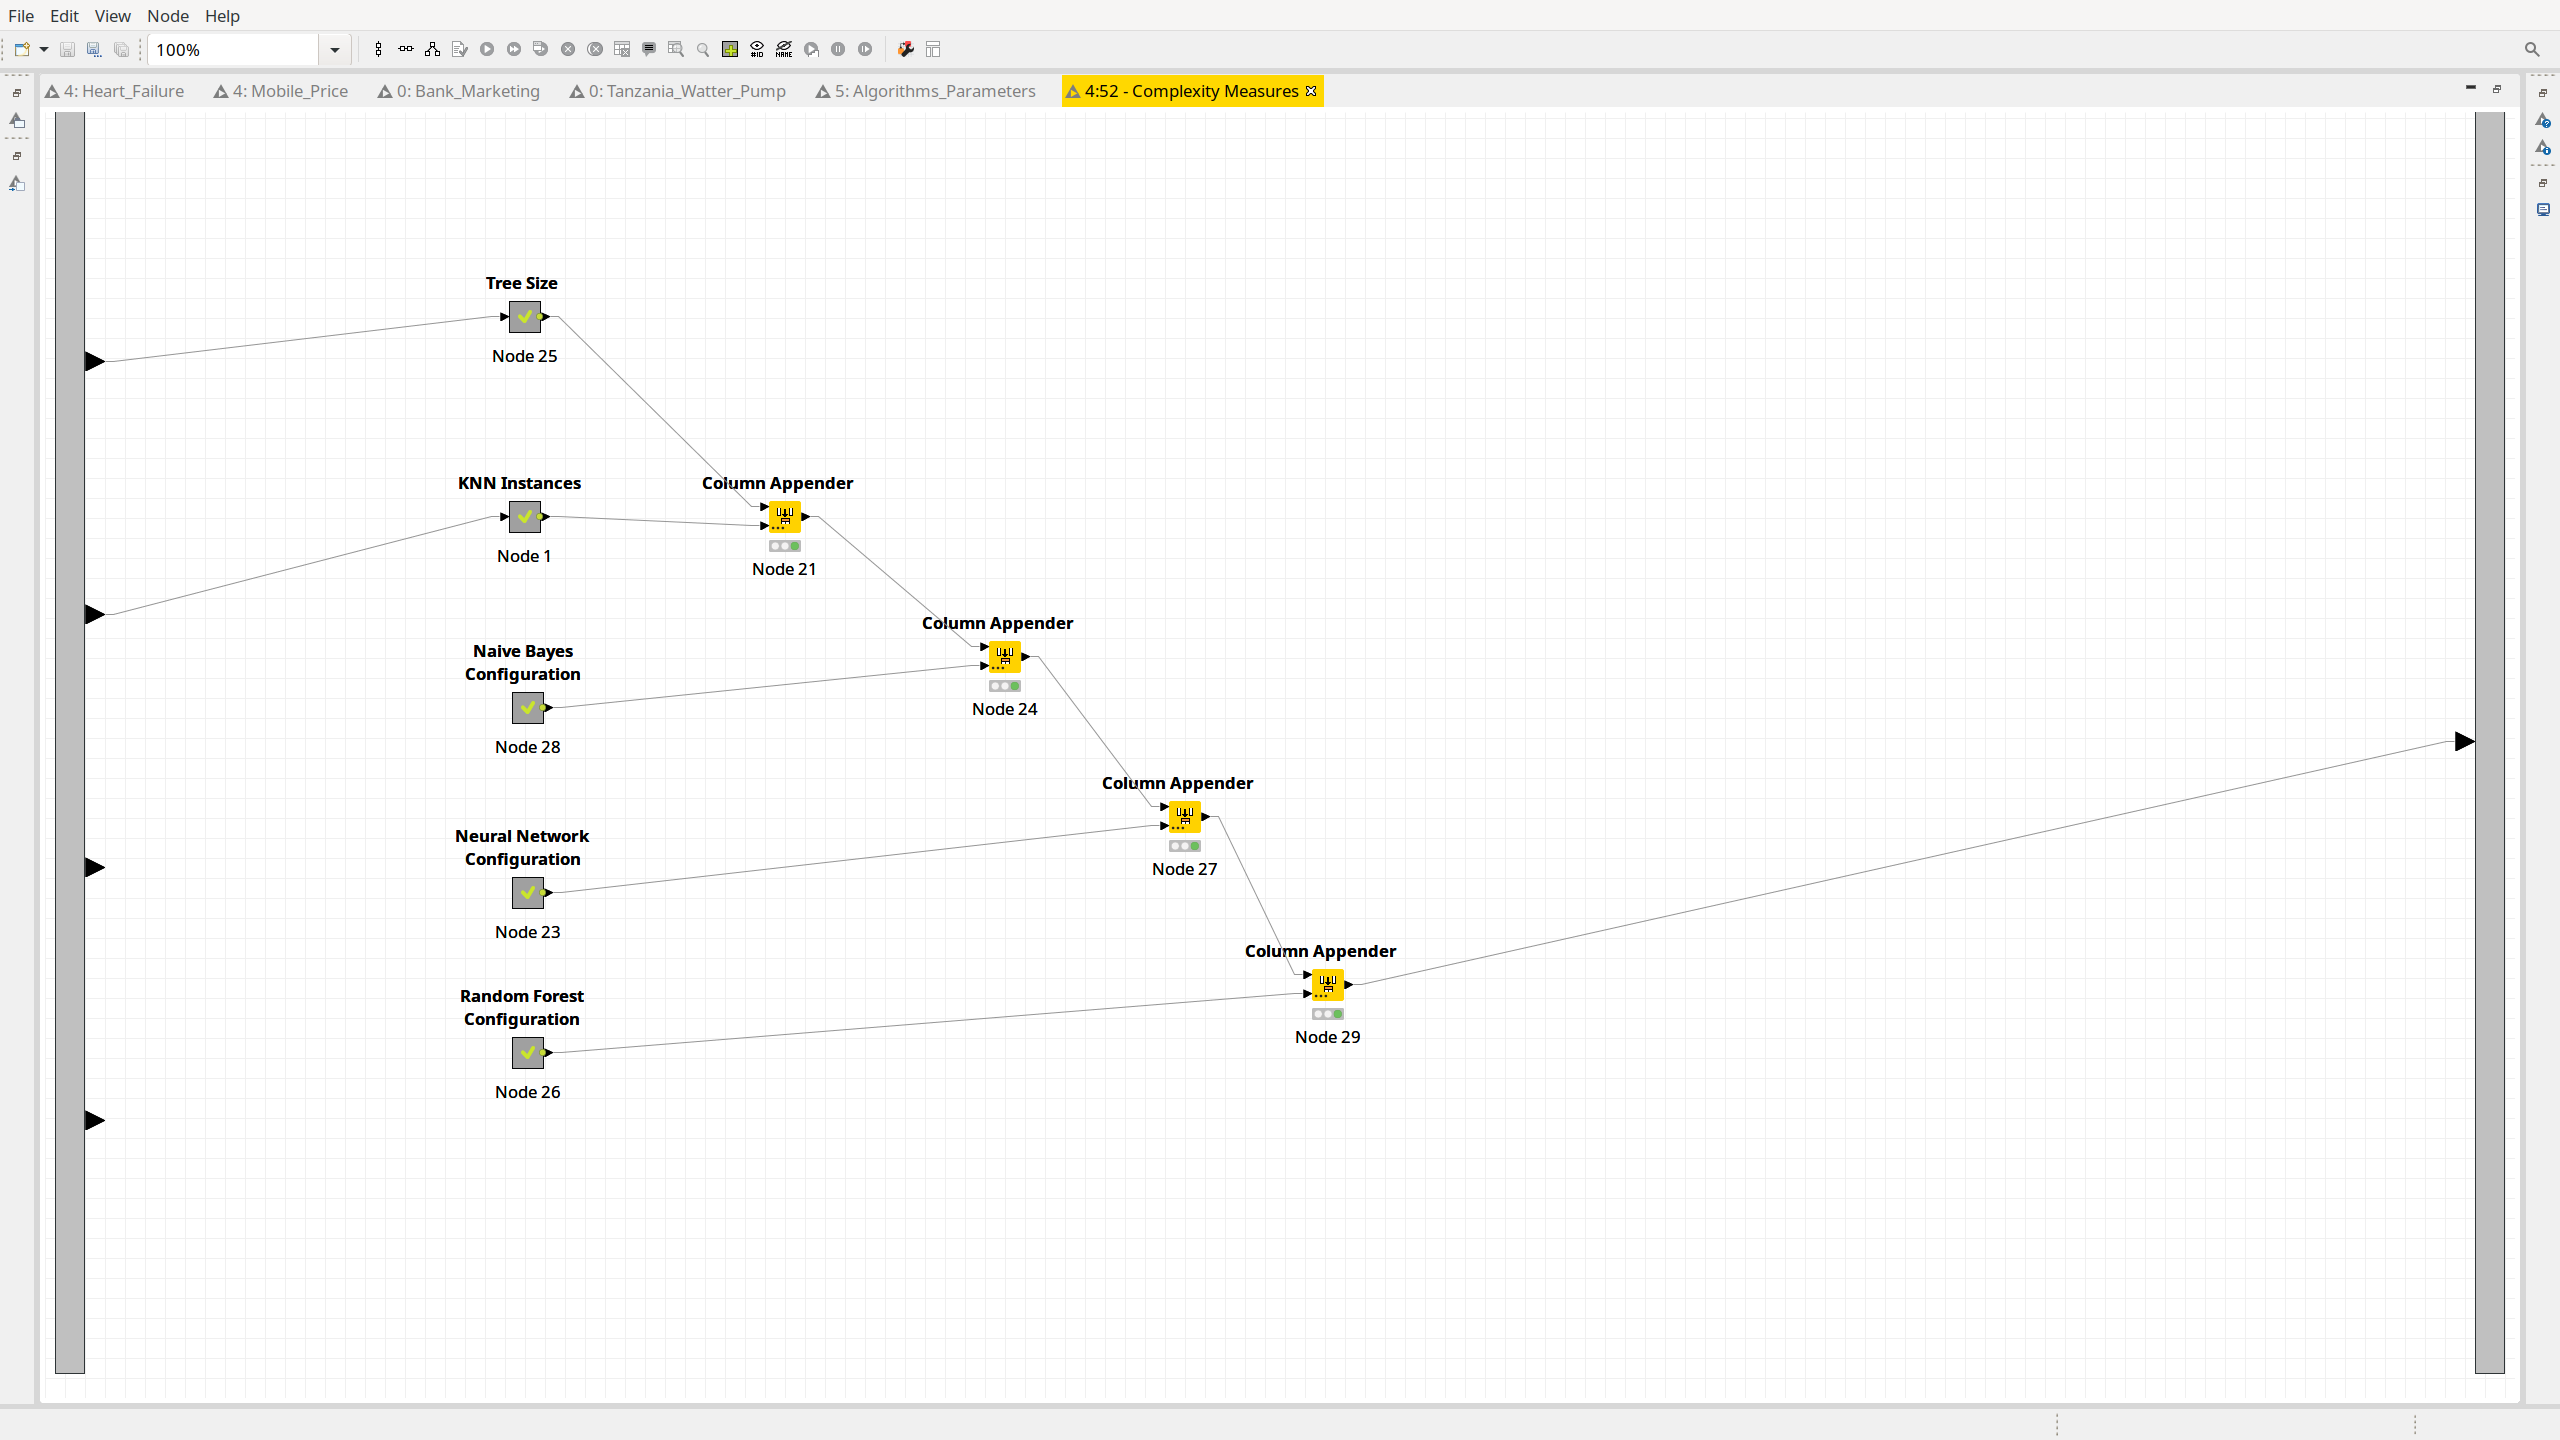
\includegraphics[width=1.0\textwidth]{\ipScreenshots/complexity_measures.png}
	\caption{Nodo \texttt{Complexity Measures}}
	\label{fig:complexity_measures}
\end{figure}

En el nodo de la figura \ref*{fig:complexity_measures} se obtienen las medidas escogidas para medir la complejidad de los algoritmos. Las asociadas al árbol de decisión y al clasificador KNN se generan de forma automática a partir de los datos procedentes de los nodos predictores mientras que el resto hay que introducirlas a mano. 

\begin{figure}[h!]
	\centering
	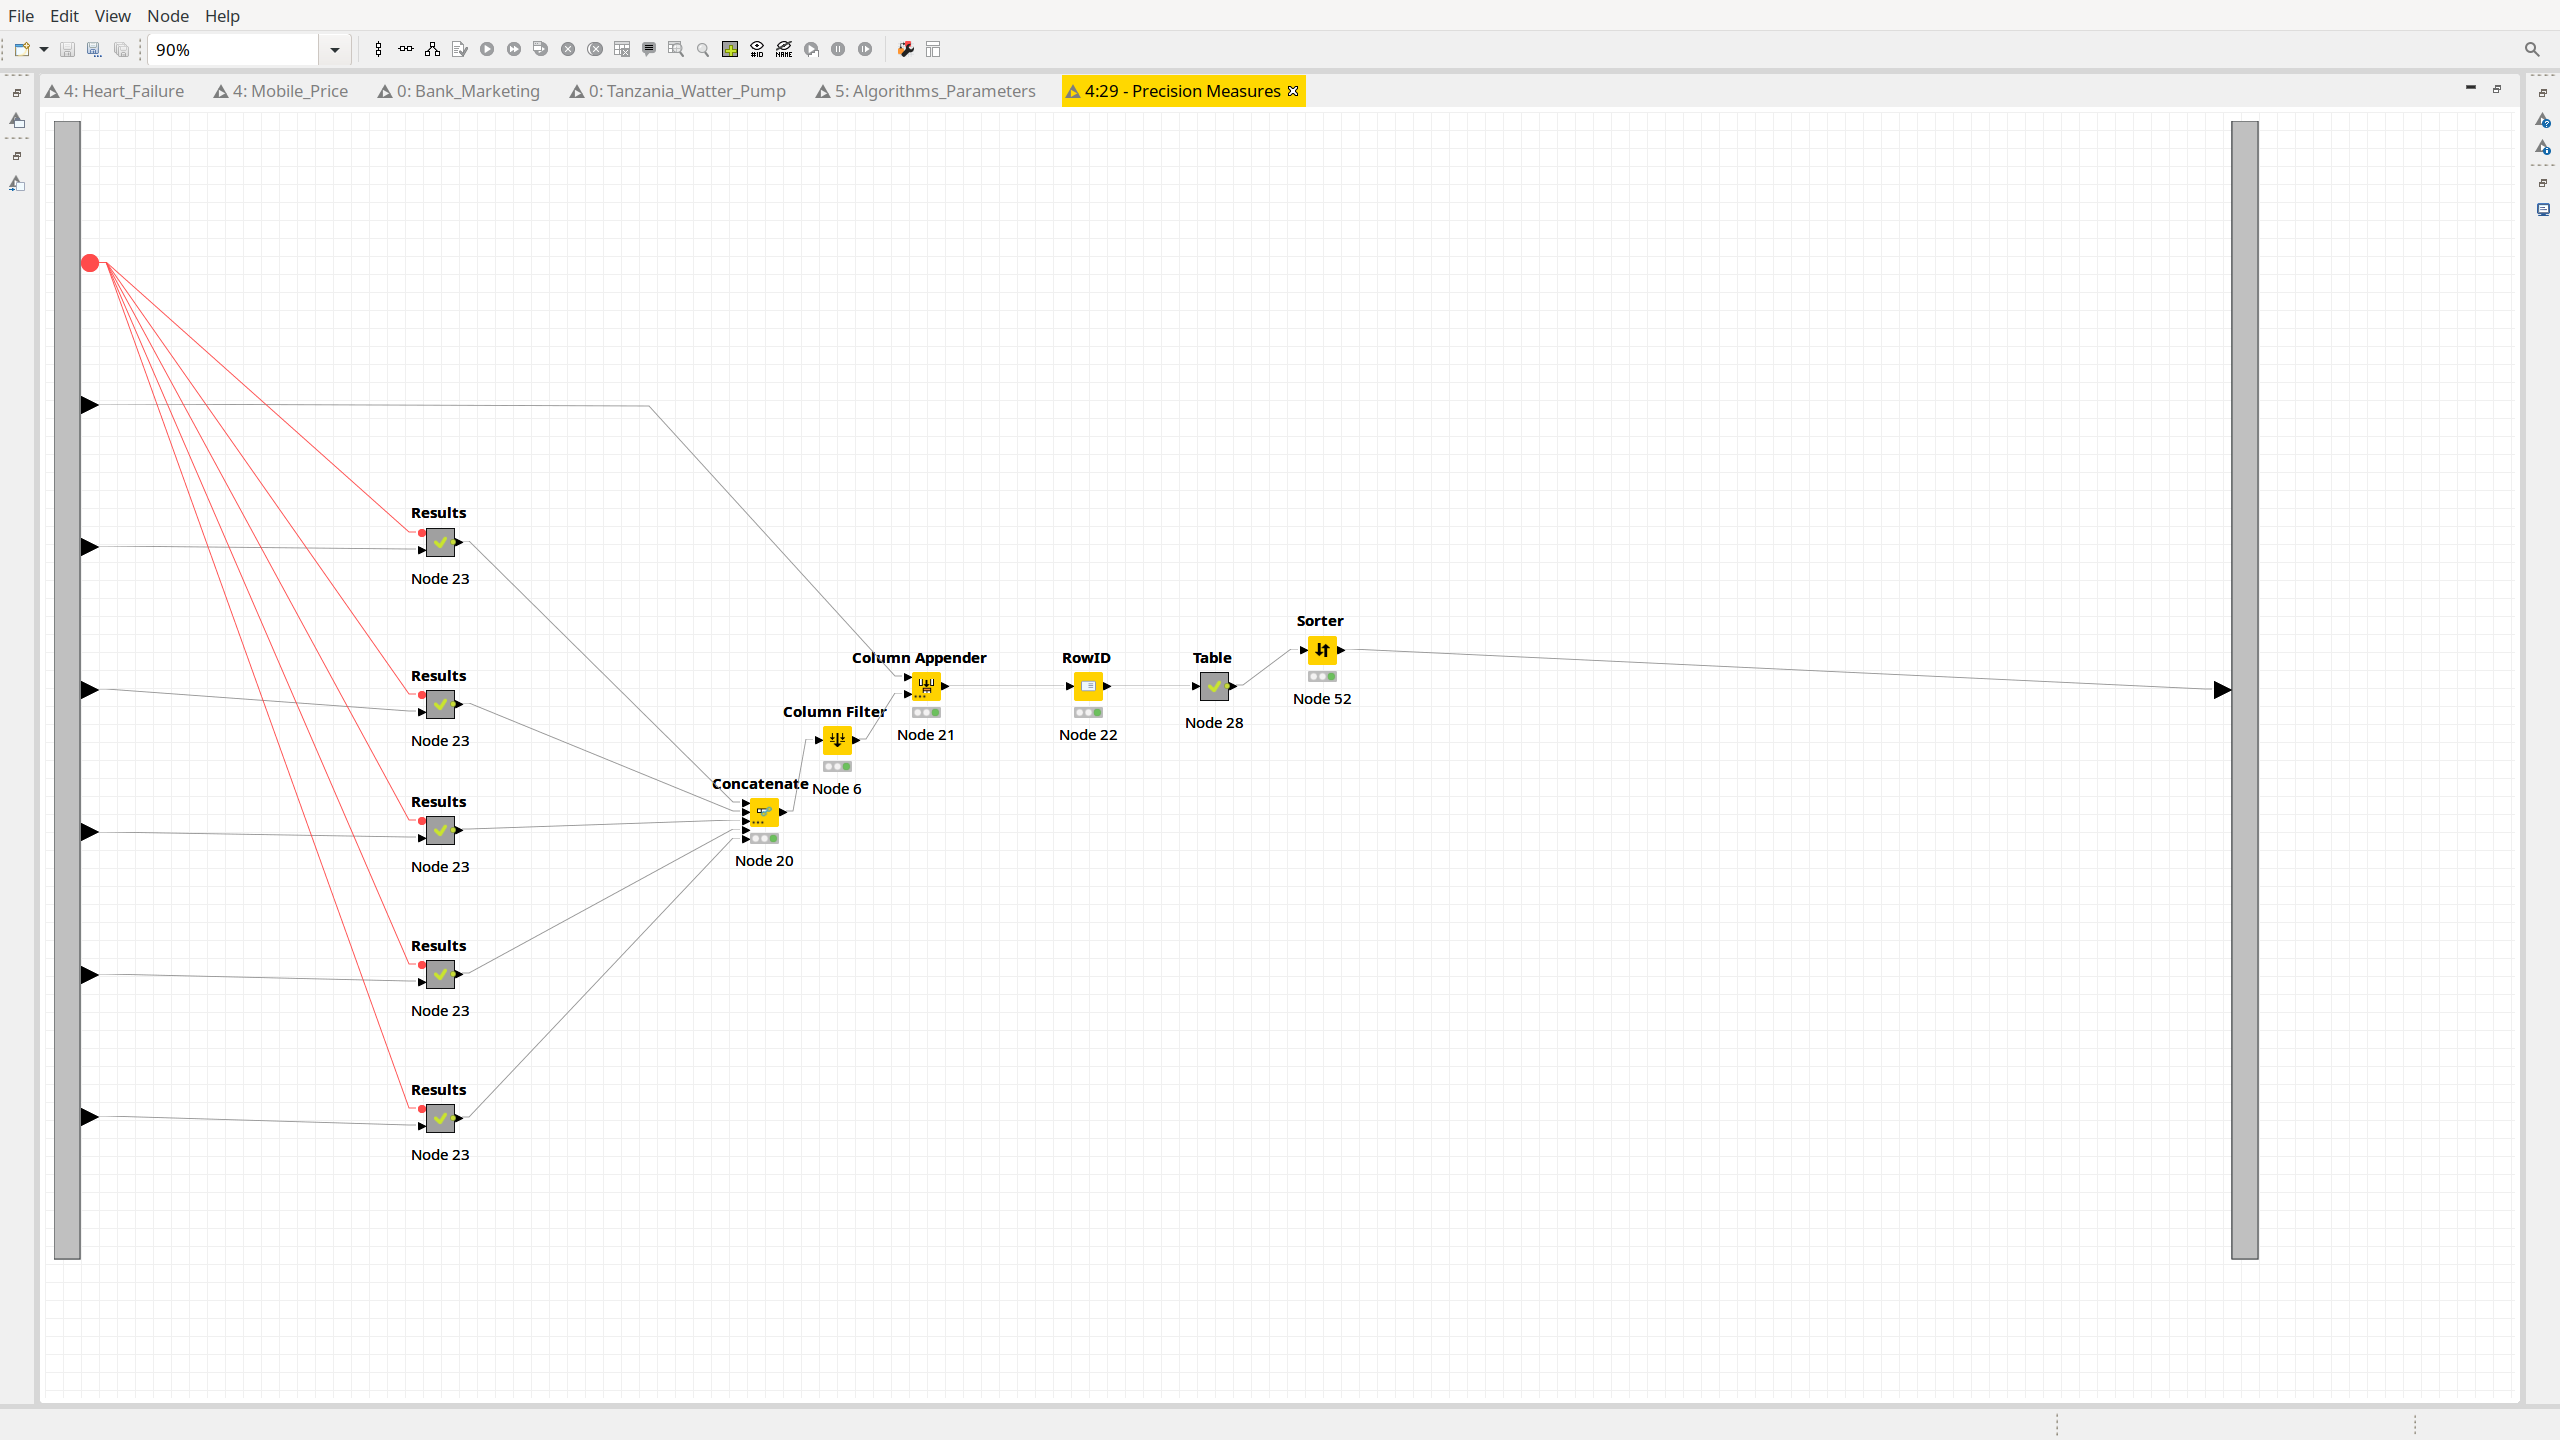
\includegraphics[width=1.0\textwidth]{\ipScreenshots/precision_measures.png}
	\caption{Nodo \texttt{Precision Measures}}
	\label{fig:precision_measures}
\end{figure}

En el nodo capturado en la \ref*{fig:precision_measures} las medidas relaccionadas con el rendimiento de los clasificadores.

\begin{figure}[h!]
	\centering
	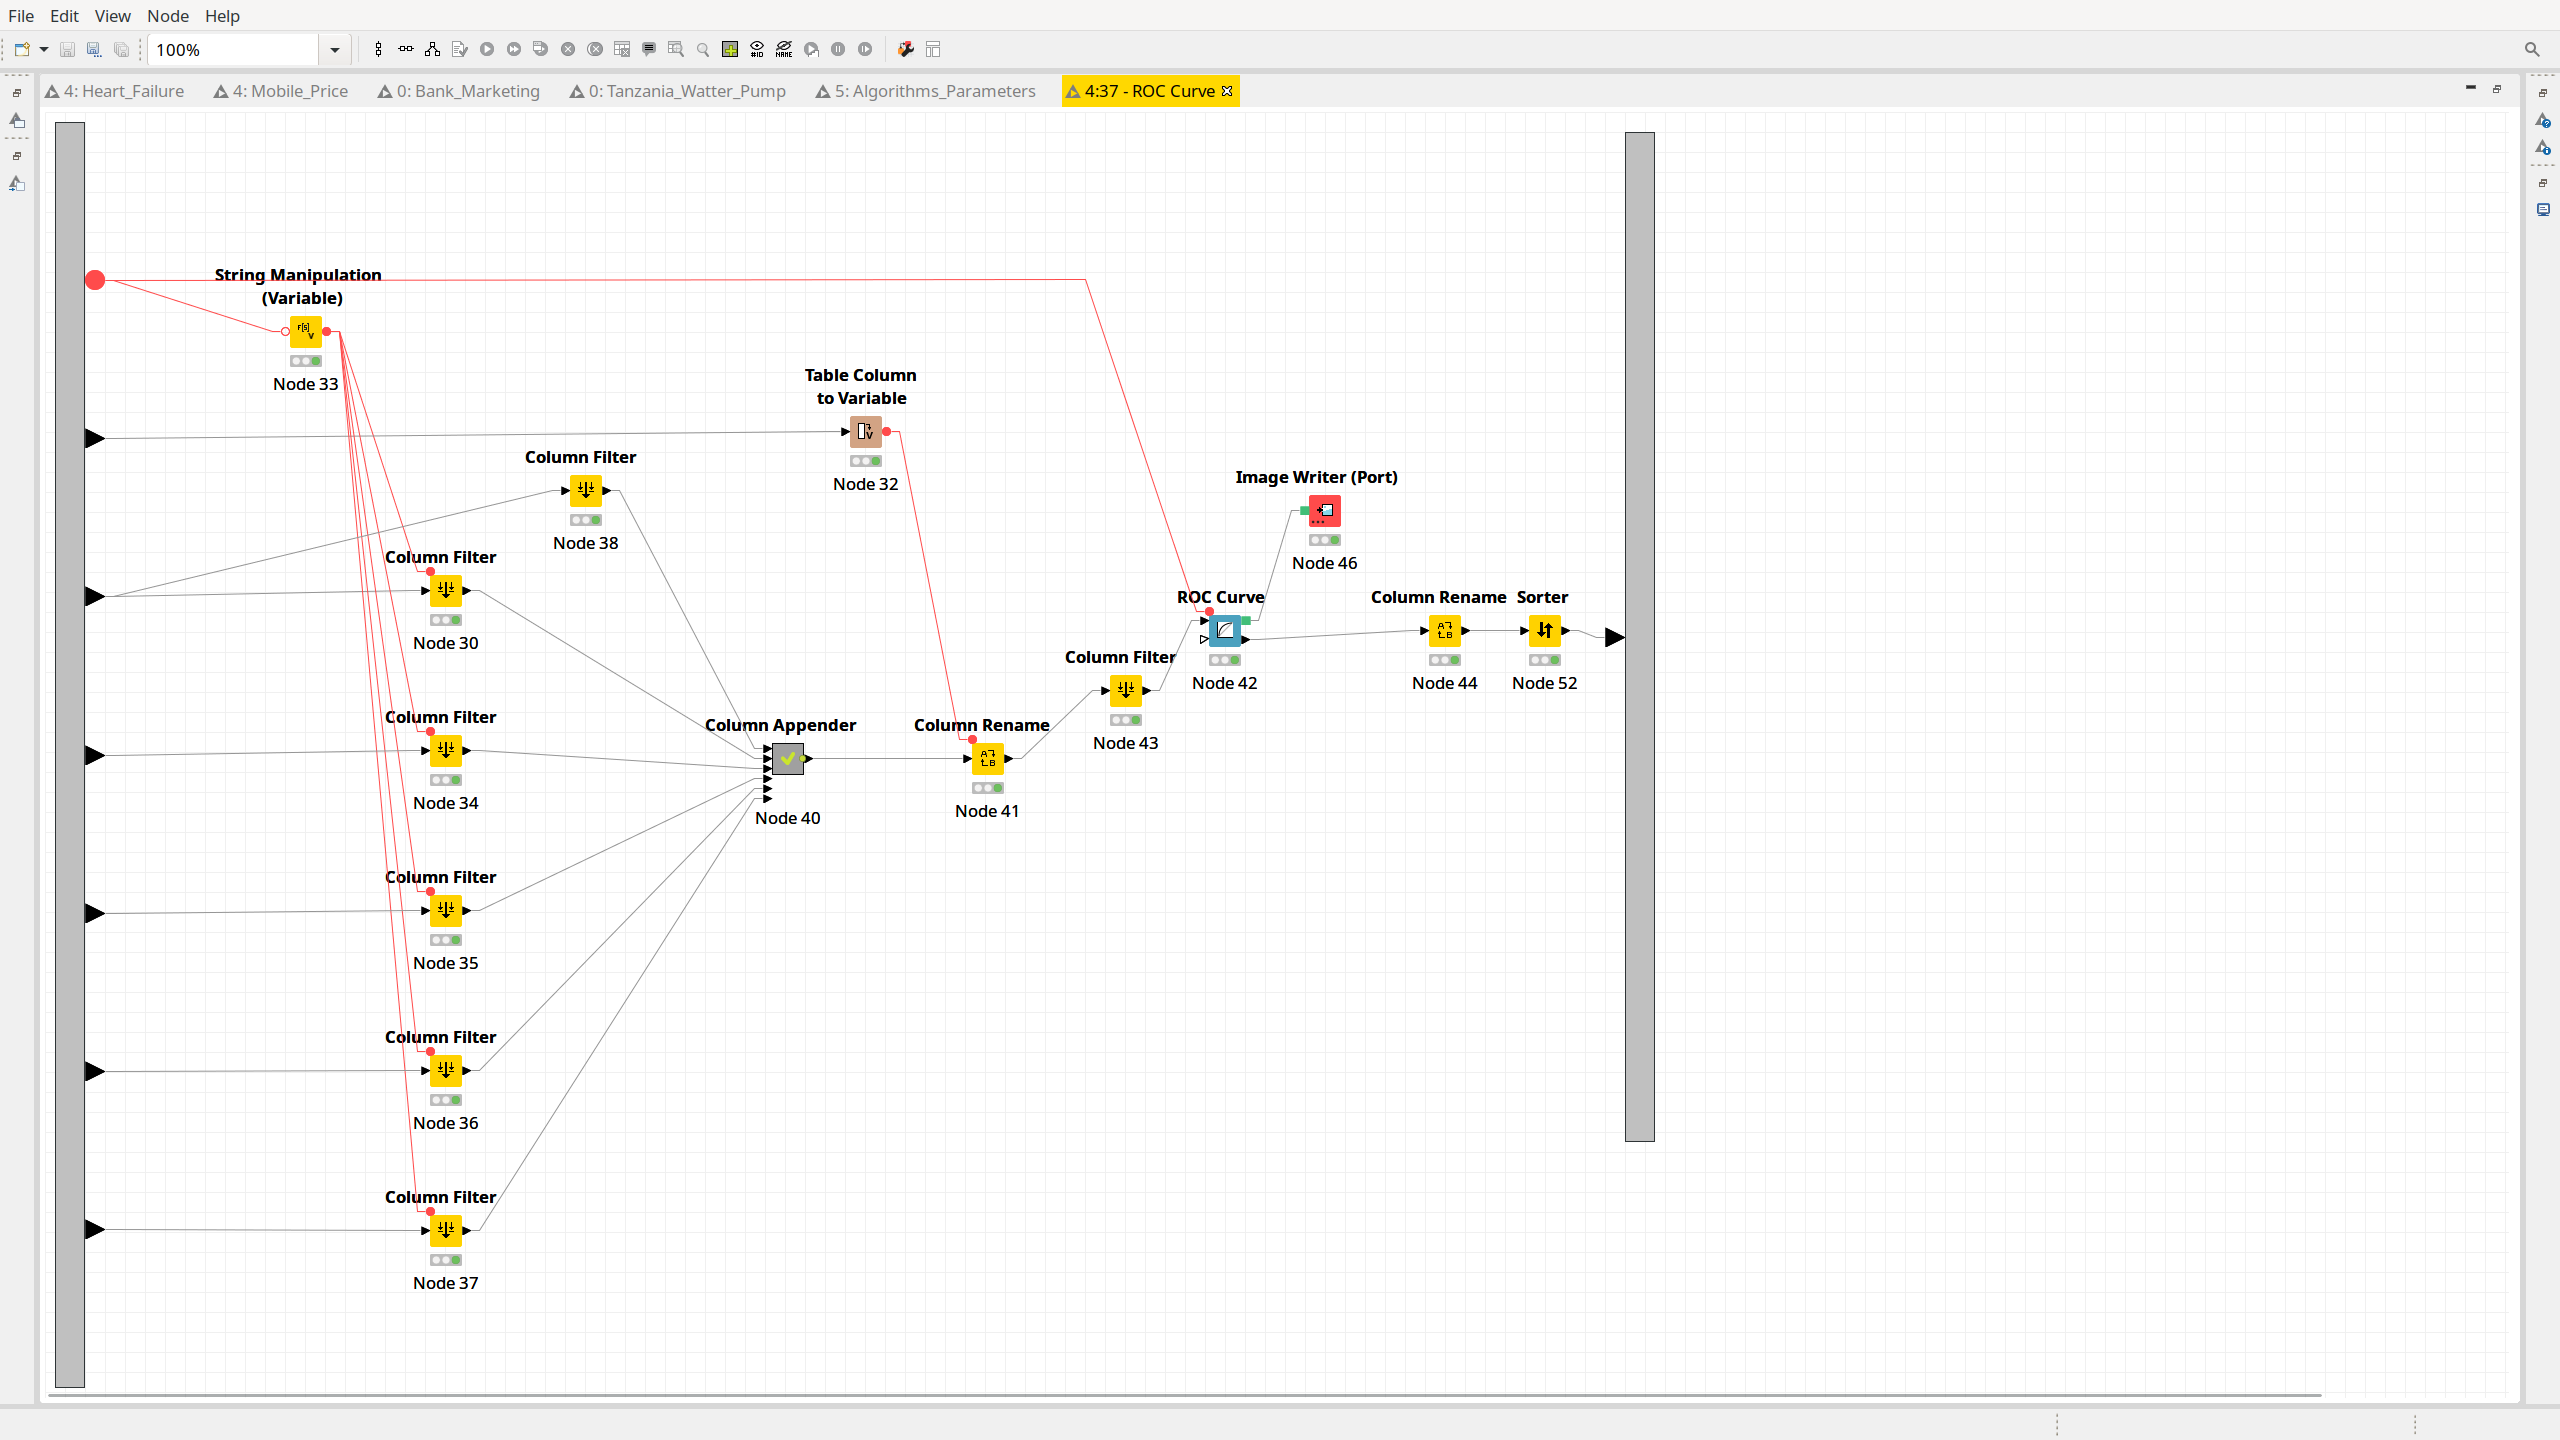
\includegraphics[width=1.0\textwidth]{\ipScreenshots/roc_curve.png}
	\caption{Nodo \texttt{Roc Curve}}
	\label{fig:roc_curve}
\end{figure}


\clearpage
\subsection{Árboles de Decisión}

\begin{figure}[h!]
	\centering
	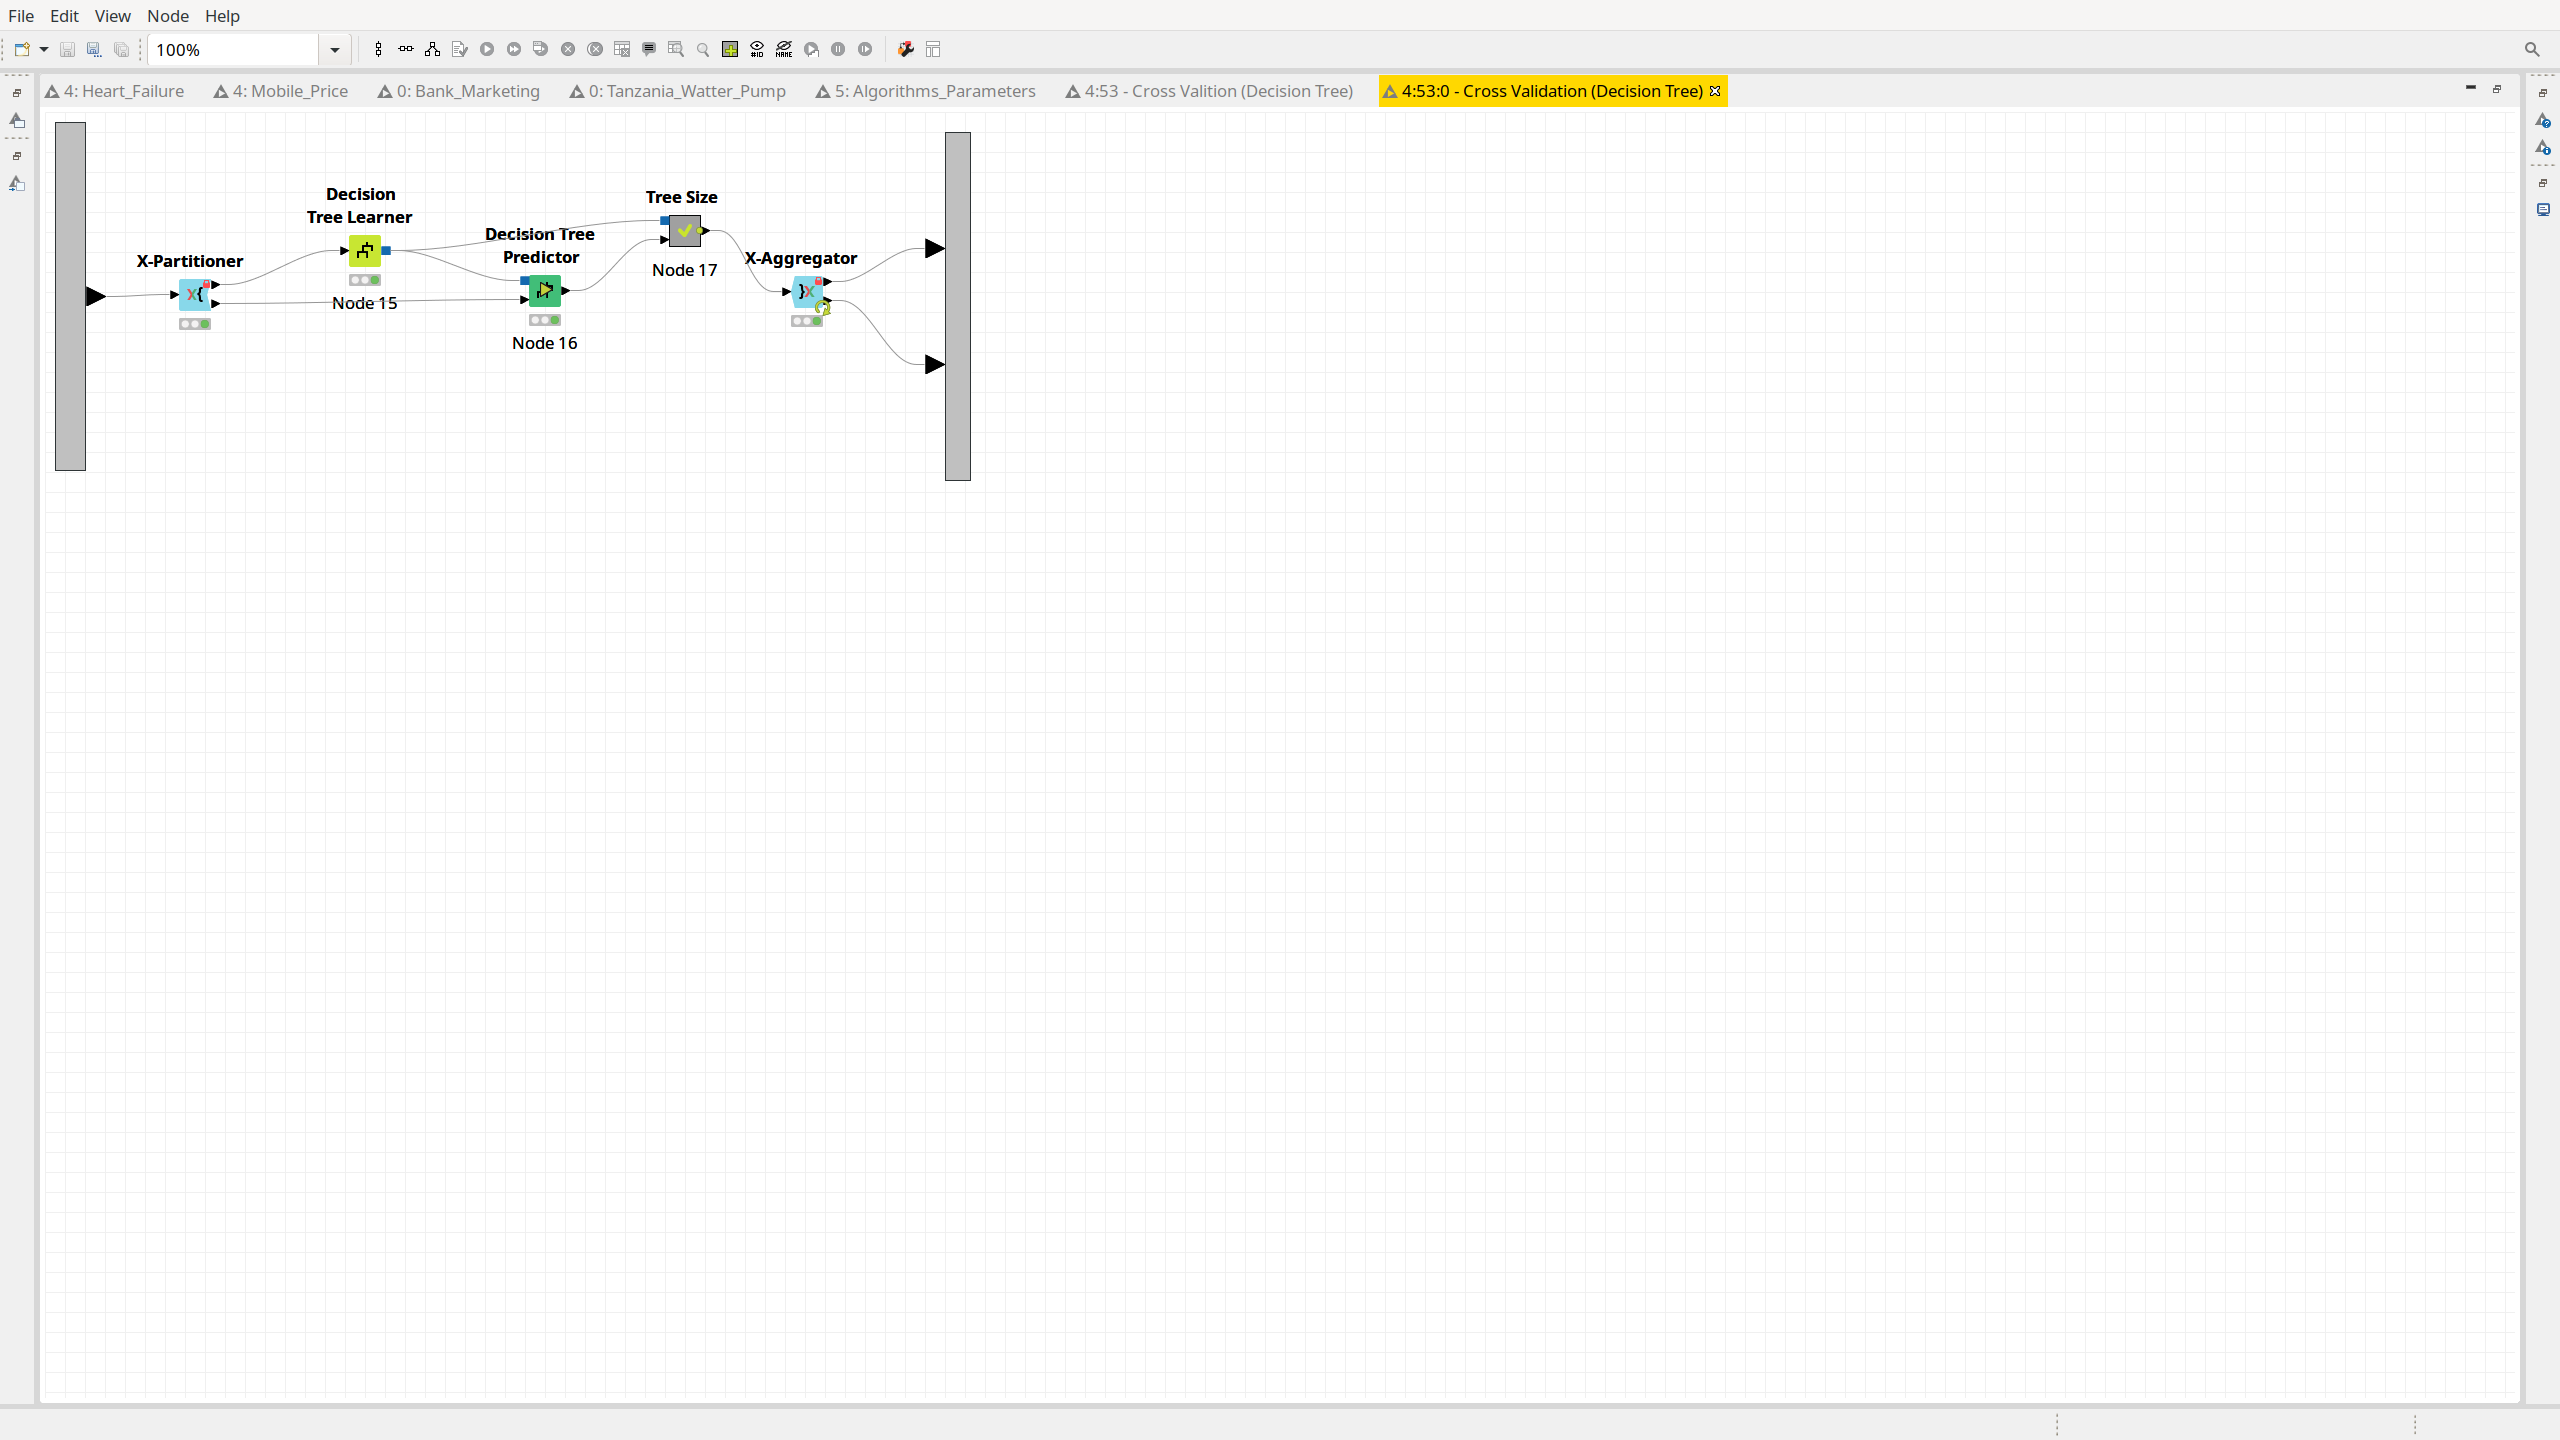
\includegraphics[width=1.0\textwidth]{\ipScreenshots/decision_tree/dt.png}
\end{figure}

\begin{figure}[h!]
	\centering
	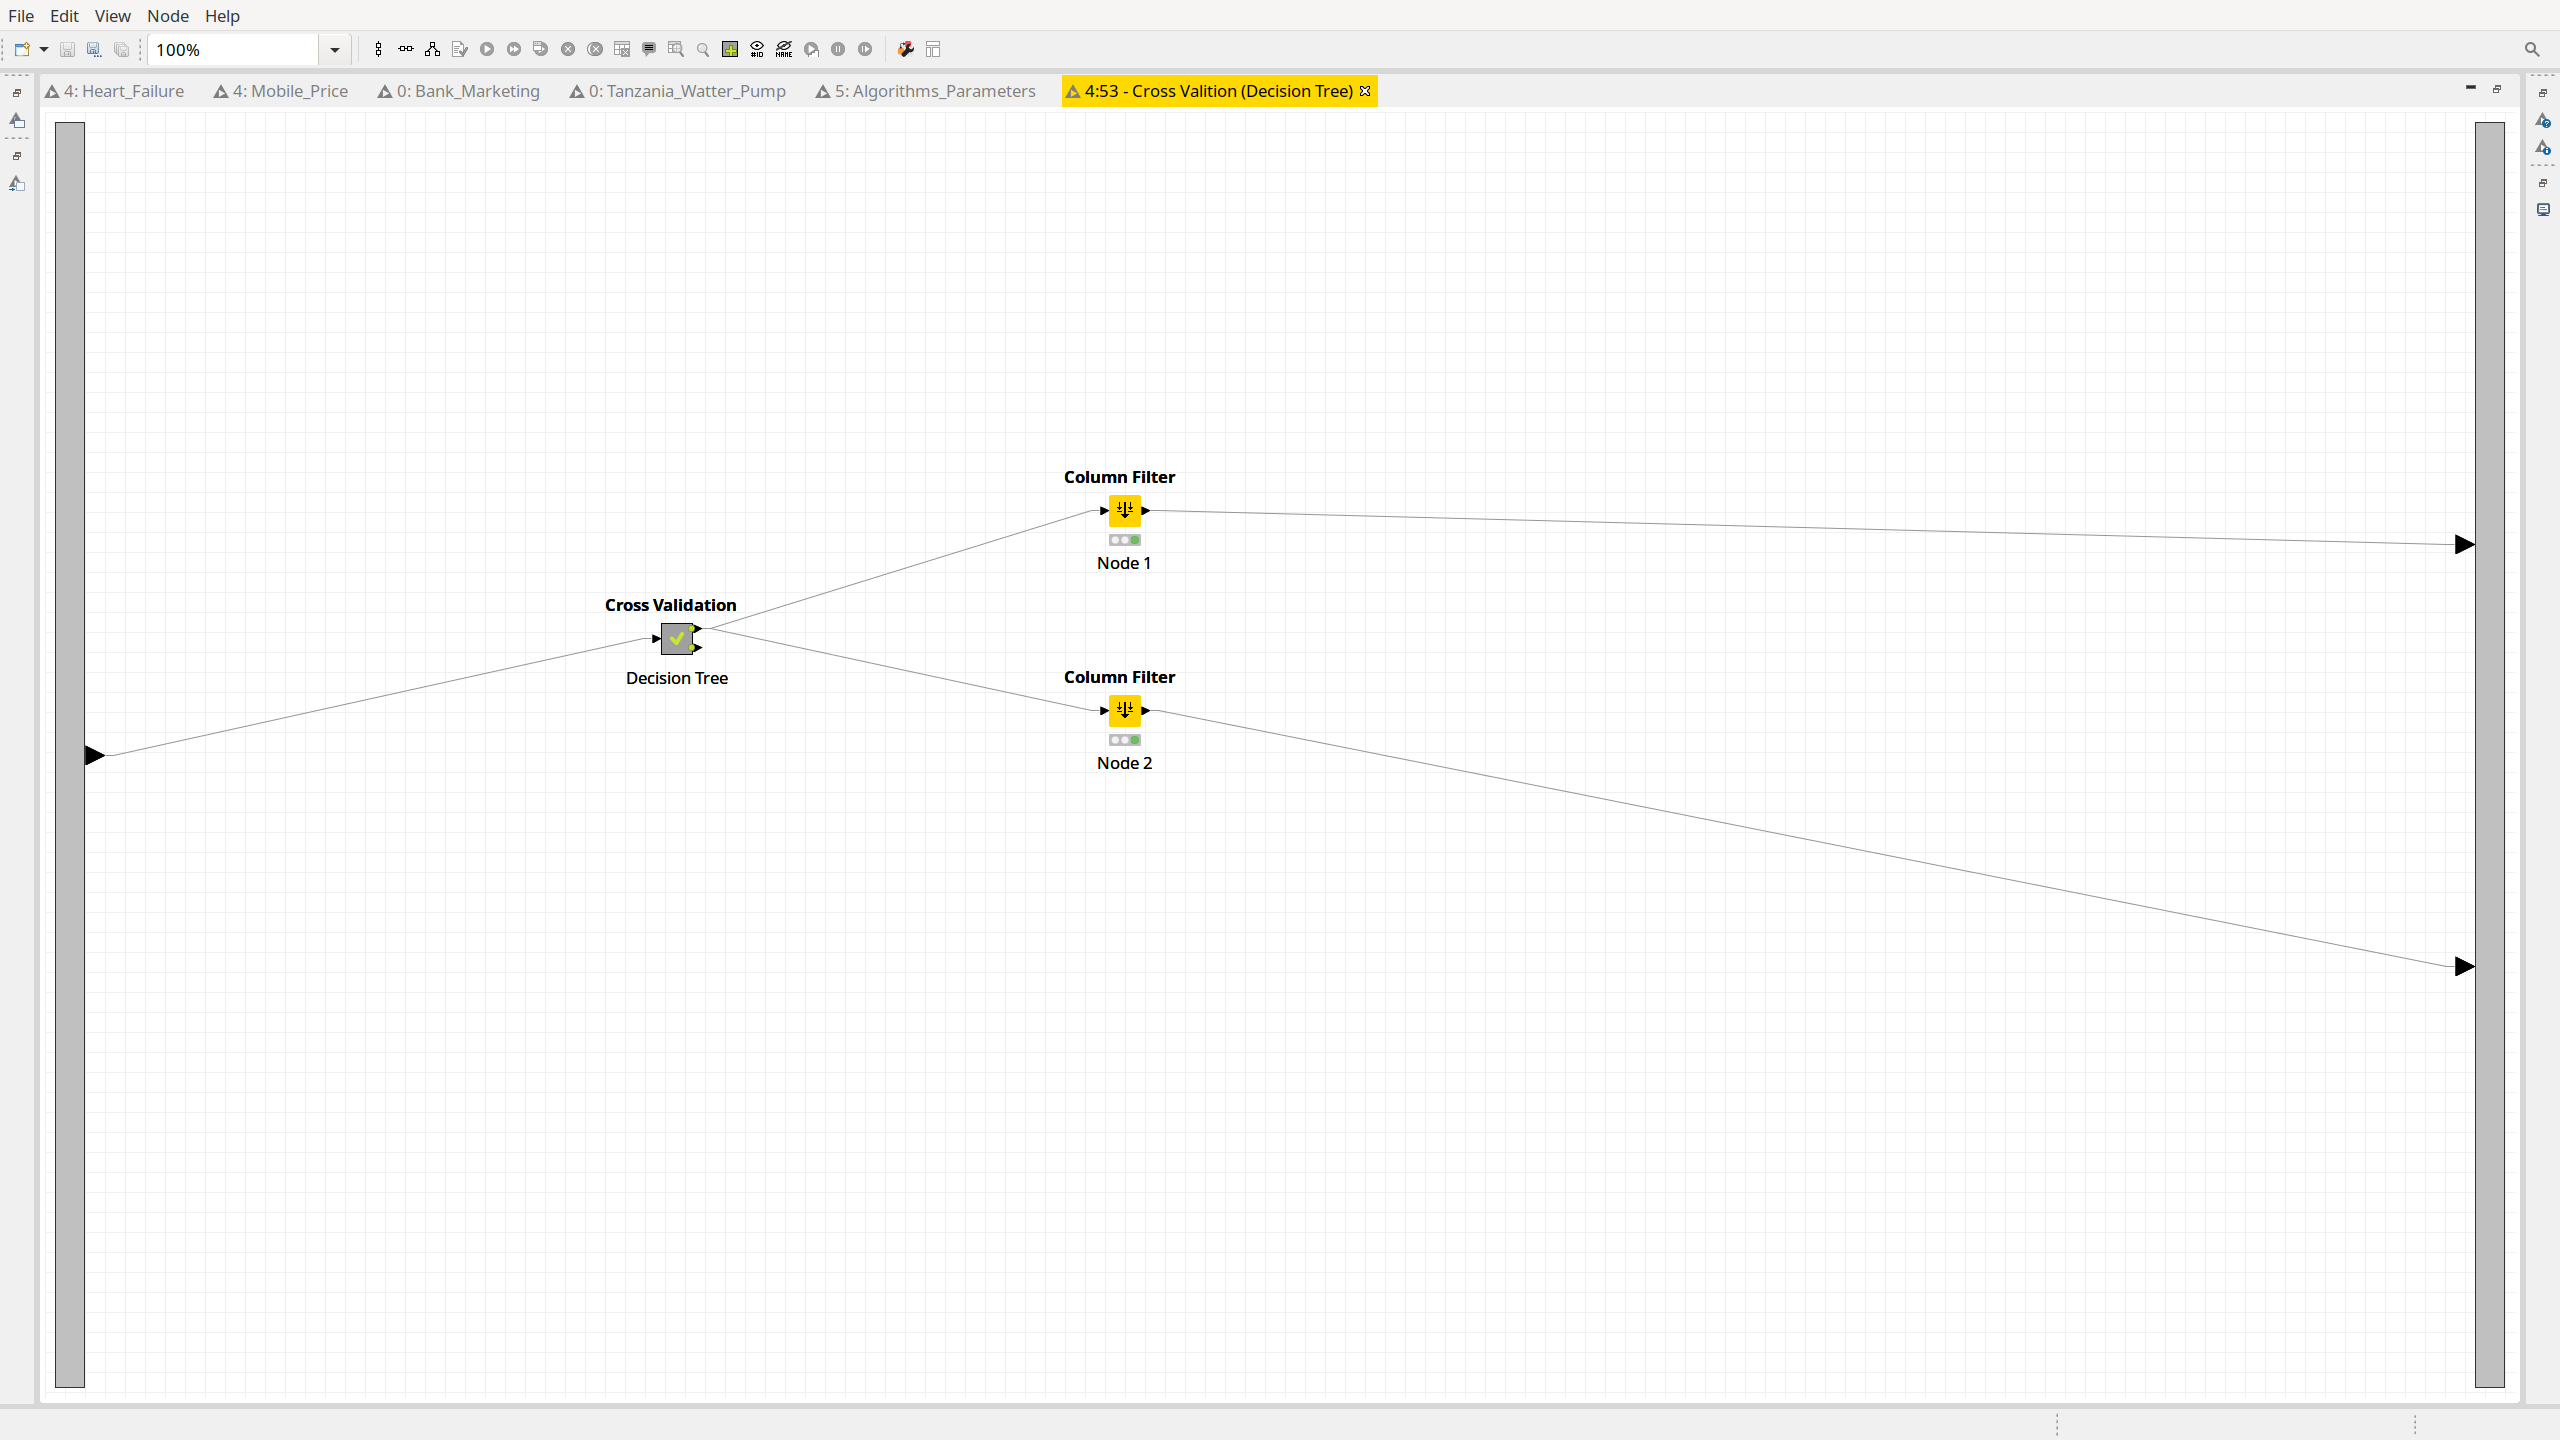
\includegraphics[width=1.0\textwidth]{\ipScreenshots/decision_tree/meta_dt.png}
\end{figure}

\begin{center}
\resizebox{\textwidth}{!}{  %Usado para ajustar la tabla a los bordes del socumento
\pgfplotstabletypeset[
	col sep={comma},
	string type,
	column type=c,
	columns={Dataset,TP,FP,TN,FN,TPR,TNR,PPV,Accuracy,F-score,G-mean,AUC},
	every head row/.style={	before row={\rowcolor[gray]{0.9}}, after row=\hline,},
	%every last row/.style={ after row=\bottomrule},
	columns/Dataset/.style = {column type=l|},
	columns/TP/.style = {dec sep align},
	columns/FP/.style = {dec sep align},
	columns/TN/.style = {dec sep align},
	columns/FN/.style = {dec sep align},
	columns/TPR/.style = {precision = 4,fixed zerofill=true, dec sep align},
	columns/TNR/.style = {precision = 4,fixed zerofill=true, dec sep align},
	columns/PPV/.style = {precision = 4,fixed zerofill=true, dec sep align},
	columns/Accuracy/.style = {precision = 4,fixed zerofill=true, dec sep align},
	columns/F-score/.style = {precision = 4,fixed zerofill=true, dec sep align},
	columns/G-mean/.style = {precision = 4,fixed zerofill=true, dec sep align},
	columns/AUC/.style = {precision = 4,fixed zerofill=true, dec sep align},
]{Cuerpo/\ipAlgorithmsResults/Decision Tree_Results.csv}
}
\end{center}


\clearpage
\subsection{KNN}

\begin{figure}[h!]
	\centering
	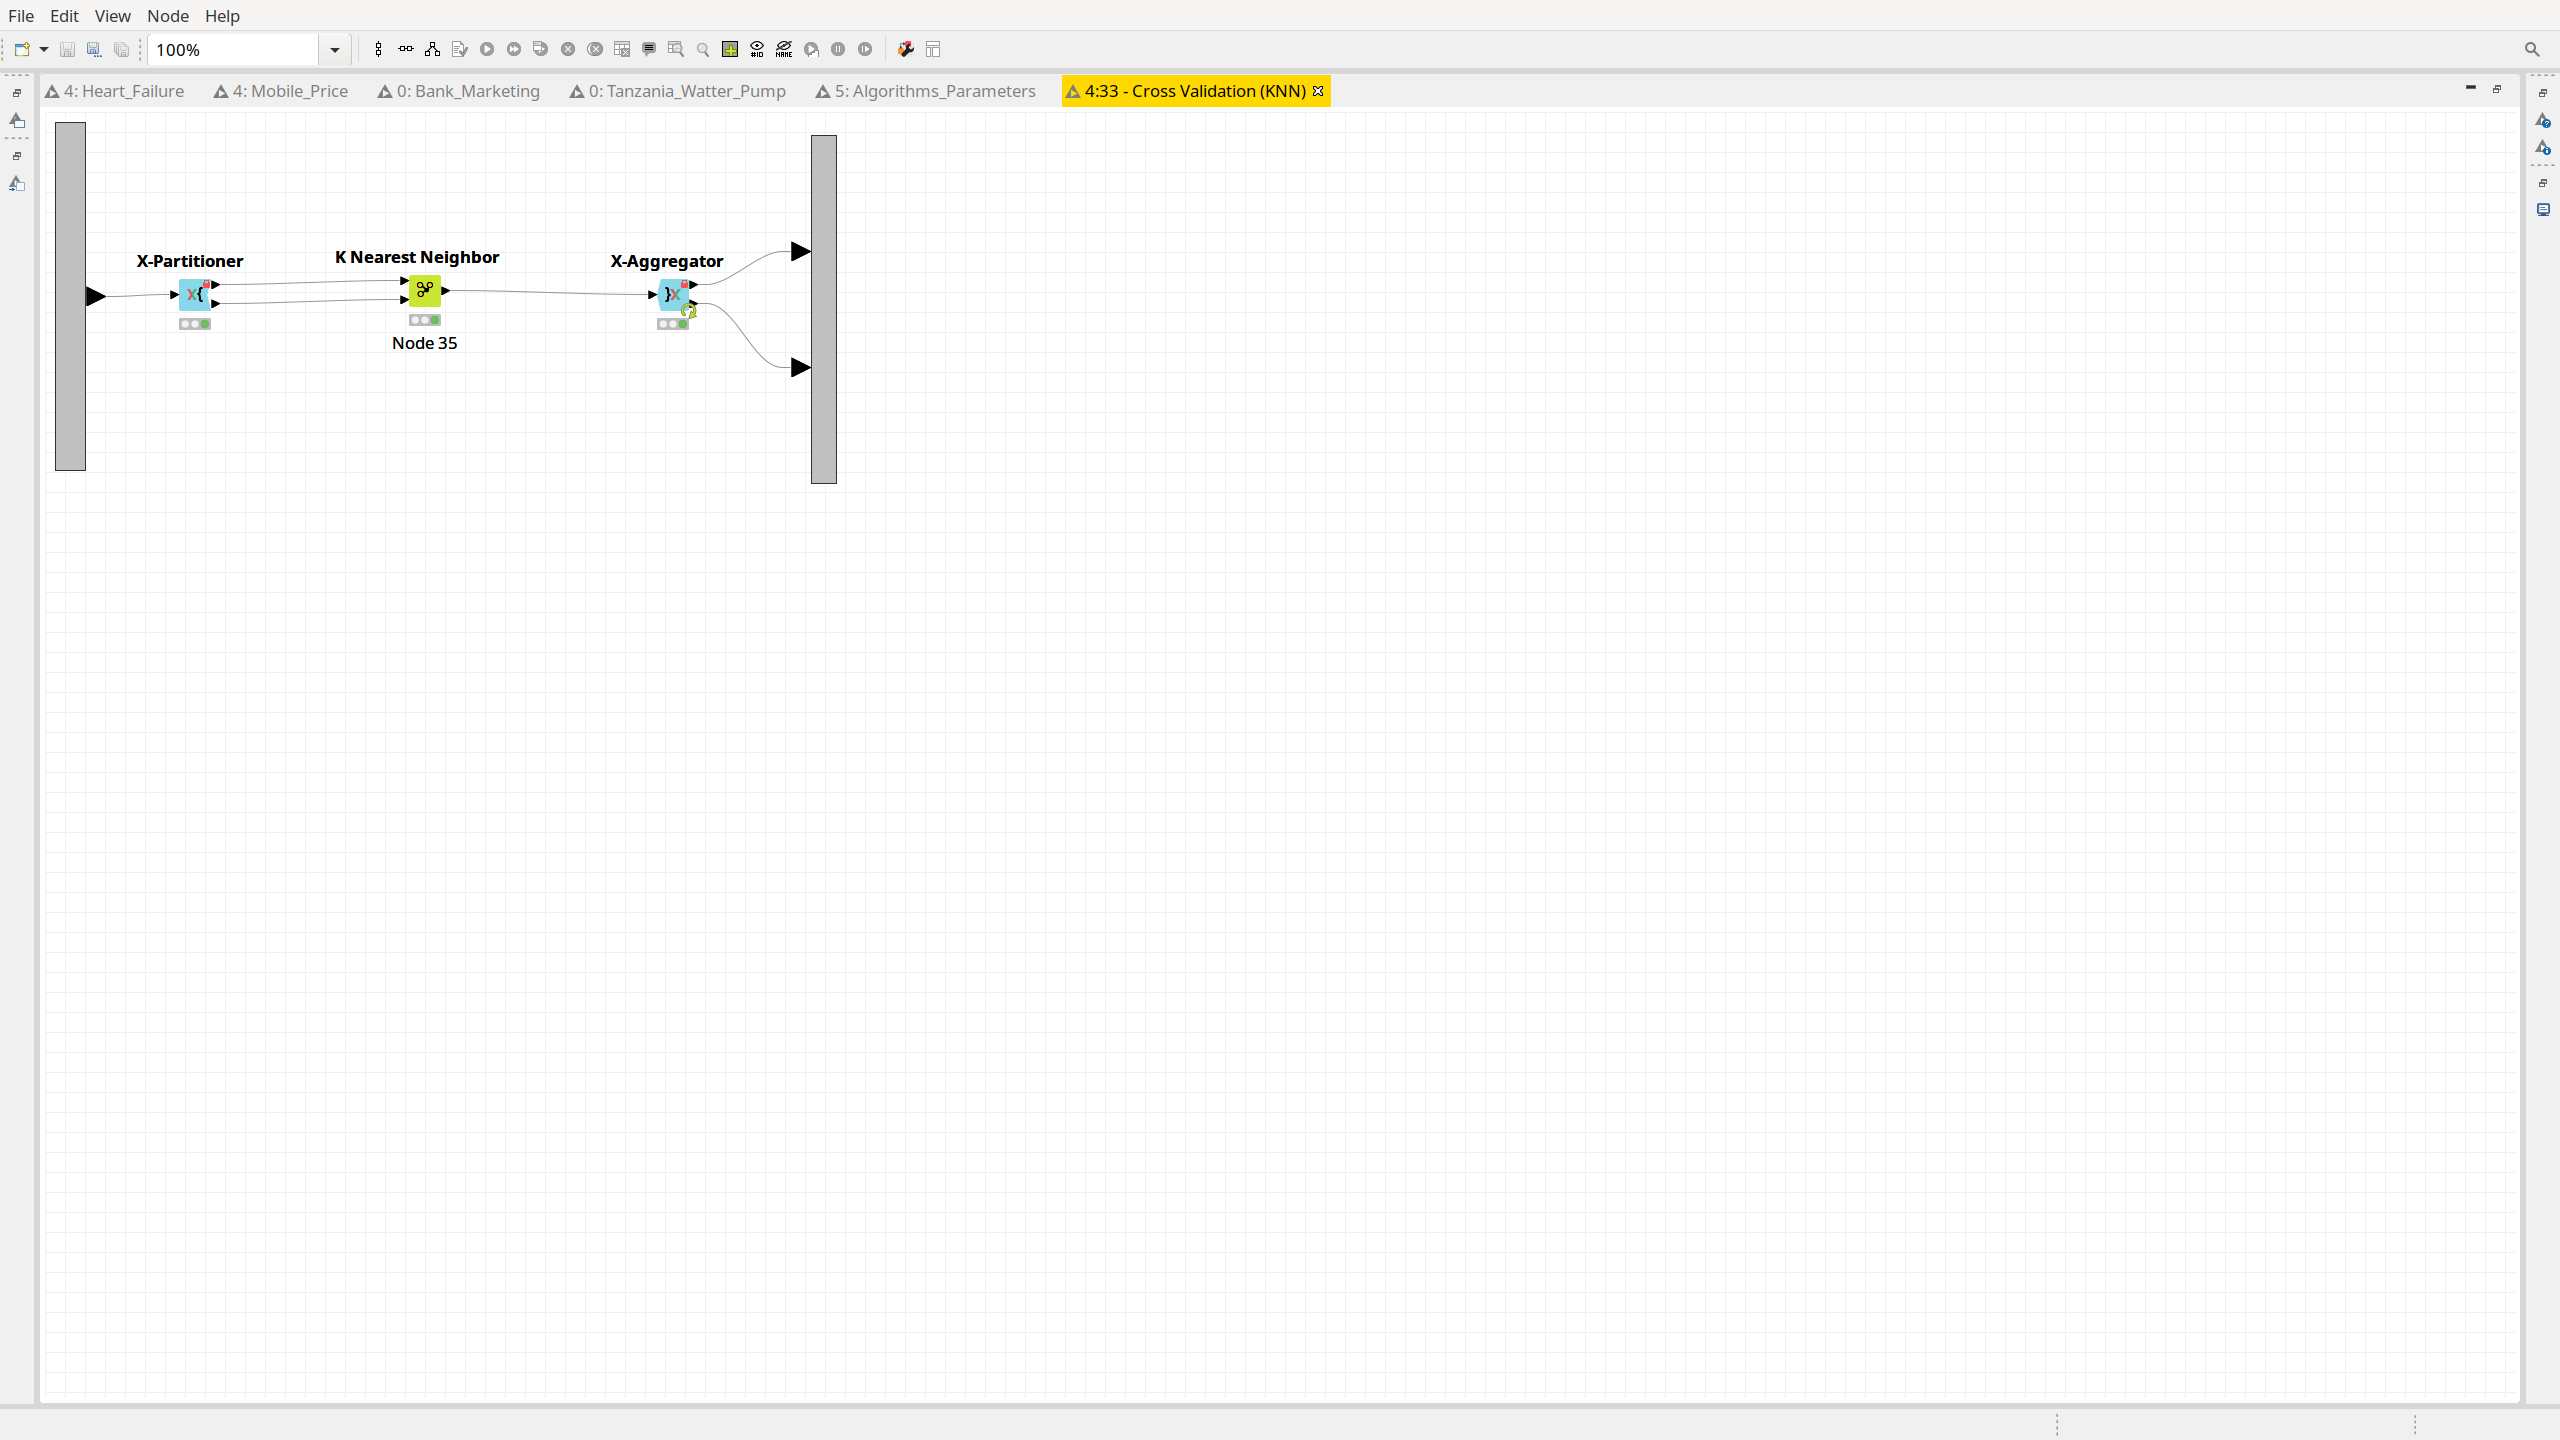
\includegraphics[width=1.0\textwidth]{\ipScreenshots/knn/knn.png}
\end{figure}

\begin{figure}[h!]
	\centering
	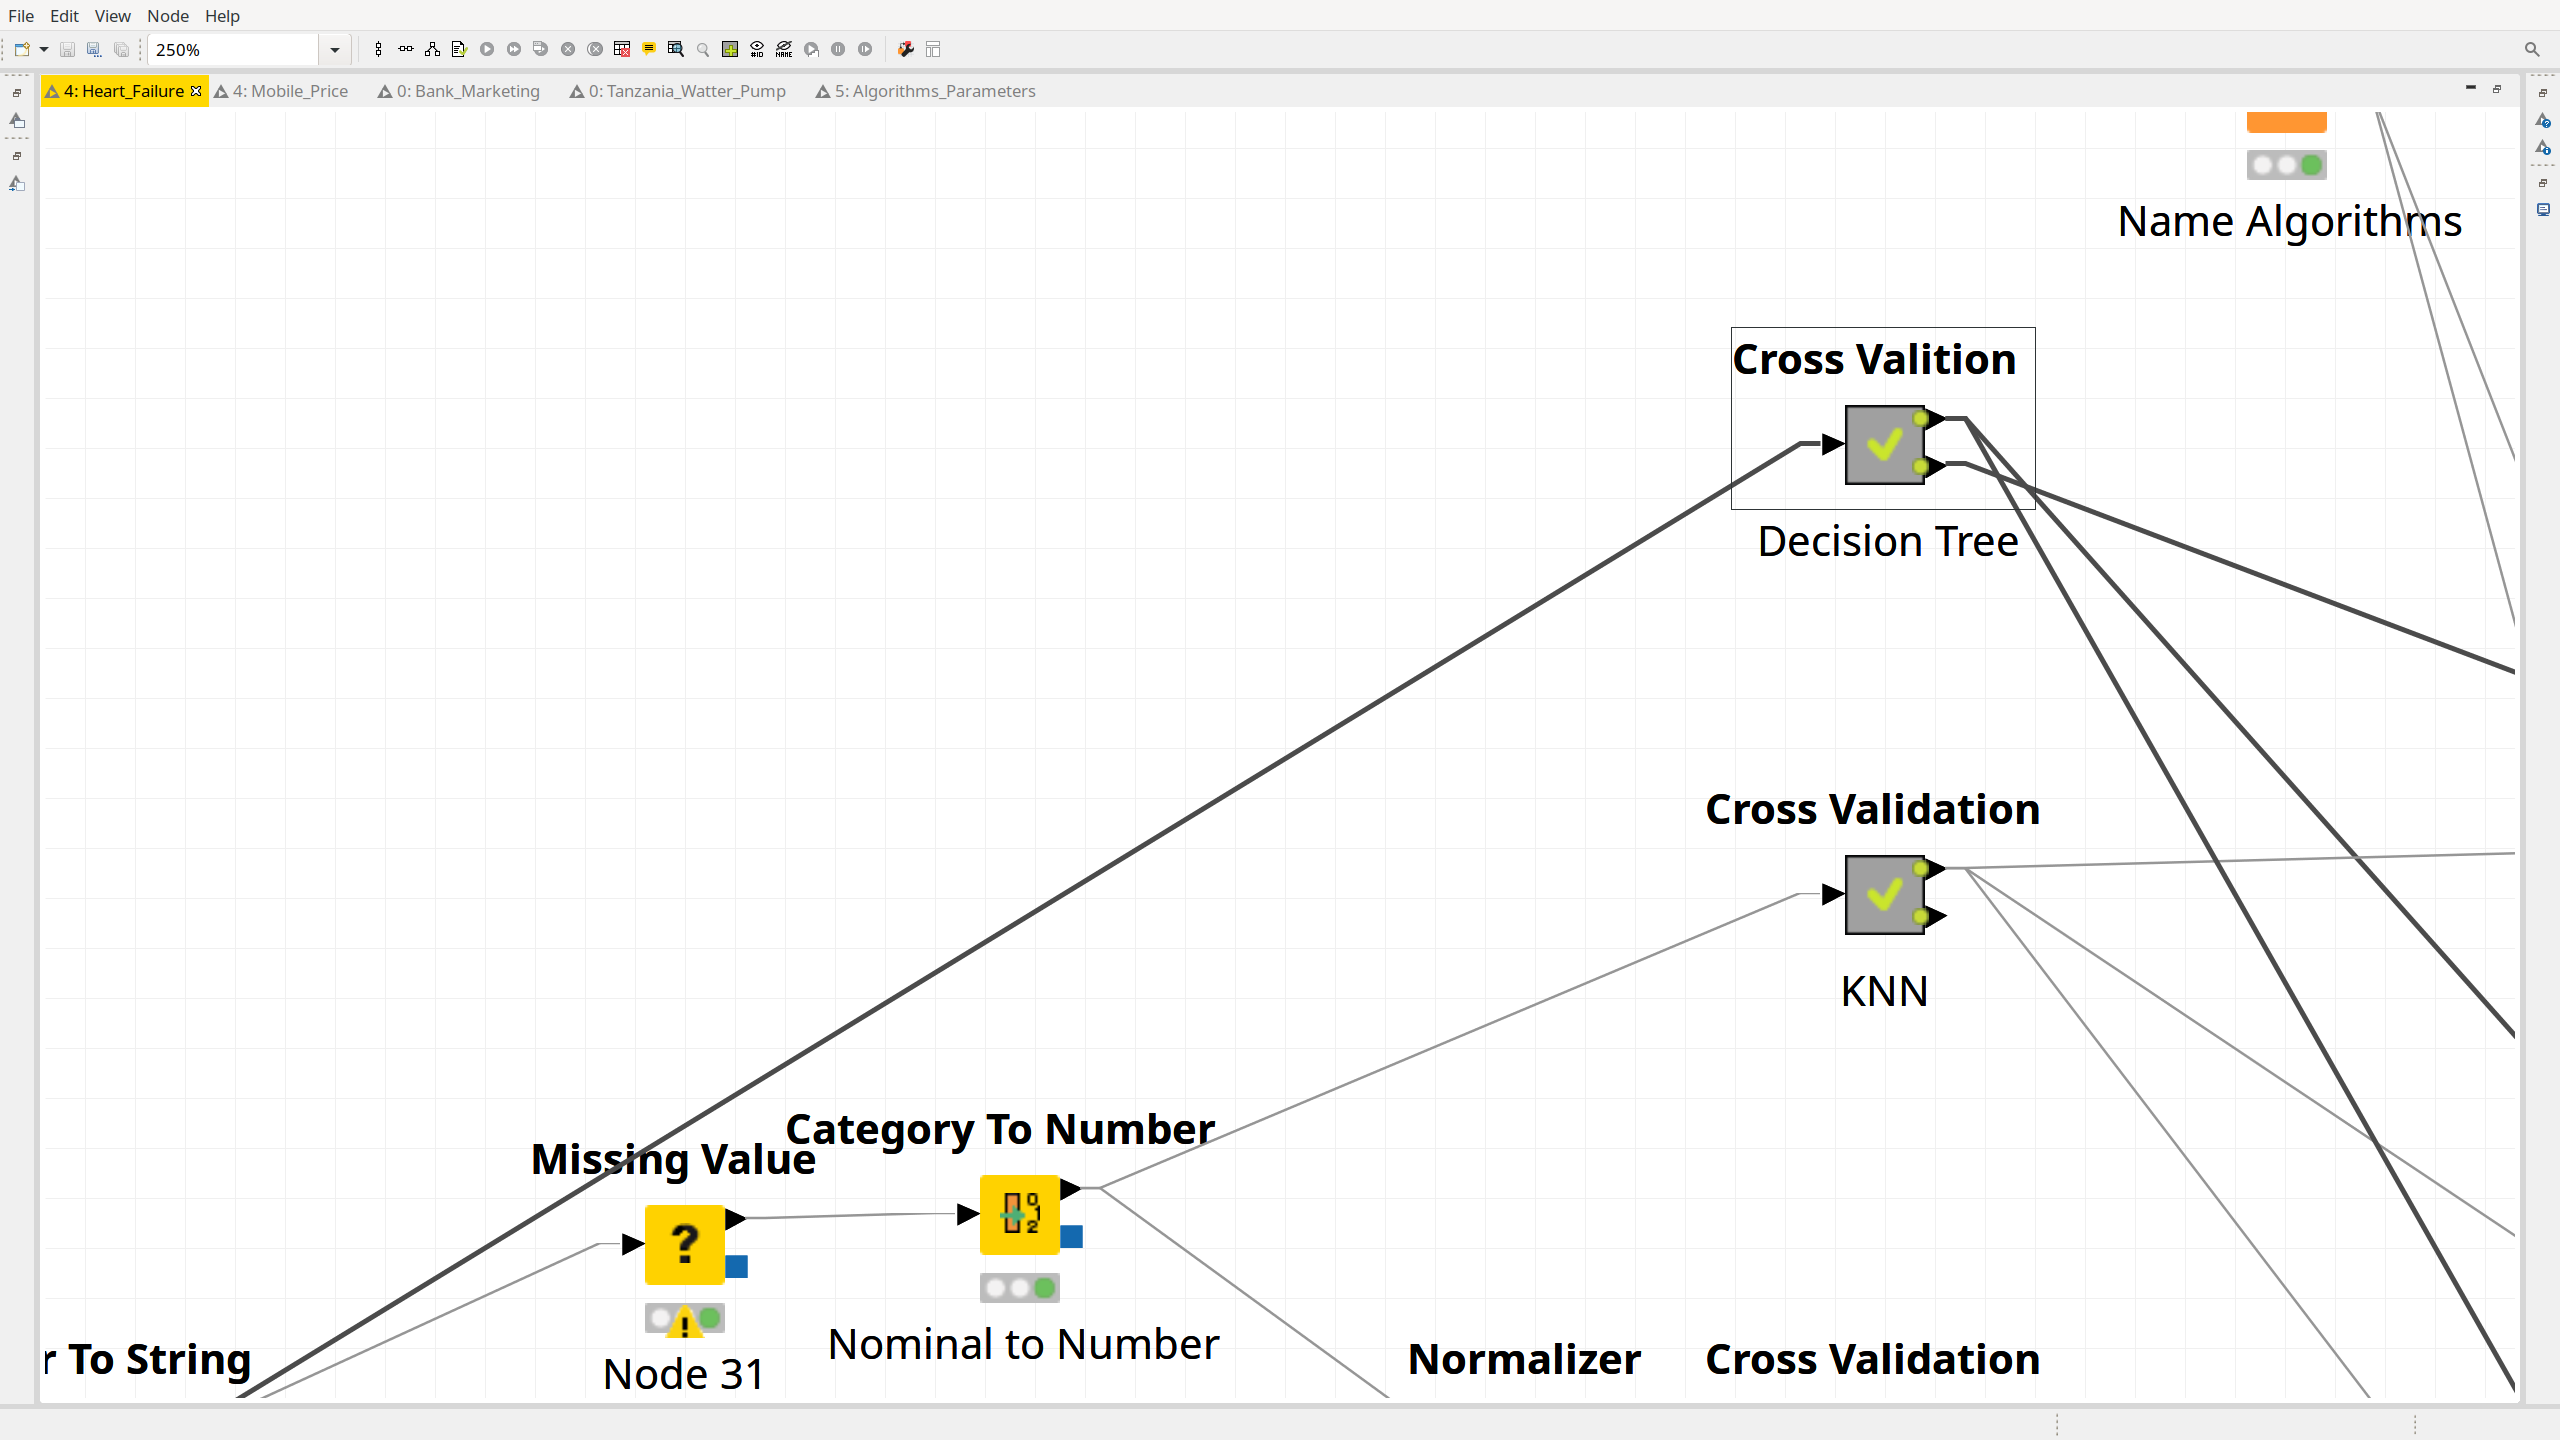
\includegraphics[width=1.0\textwidth]{\ipScreenshots/knn/pre_knn.png}
\end{figure}

\begin{center}
\resizebox{\textwidth}{!}{  %Usado para ajustar la tabla a los bordes del socumento
\pgfplotstabletypeset[
	col sep={comma},
	string type,
	column type=c,
	columns={Dataset,TP,FP,TN,FN,TPR,TNR,PPV,Accuracy,F-score,G-mean,AUC},
	every head row/.style={	before row={\rowcolor[gray]{0.9}}, after row=\hline,},
	%every last row/.style={ after row=\bottomrule},
	columns/Dataset/.style = {column type=l|},
	columns/TP/.style = {dec sep align},
	columns/FP/.style = {dec sep align},
	columns/TN/.style = {dec sep align},
	columns/FN/.style = {dec sep align},
	columns/TPR/.style = {precision = 4,fixed zerofill=true, dec sep align},
	columns/TNR/.style = {precision = 4,fixed zerofill=true, dec sep align},
	columns/PPV/.style = {precision = 4,fixed zerofill=true, dec sep align},
	columns/Accuracy/.style = {precision = 4,fixed zerofill=true, dec sep align},
	columns/F-score/.style = {precision = 4,fixed zerofill=true, dec sep align},
	columns/G-mean/.style = {precision = 4,fixed zerofill=true, dec sep align},
	columns/AUC/.style = {precision = 4,fixed zerofill=true, dec sep align},
]{Cuerpo/\ipAlgorithmsResults/KNN_Results.csv}
}
\end{center}


\clearpage
\subsection{Naive Bayes}

\begin{figure}[h!]
	\centering
	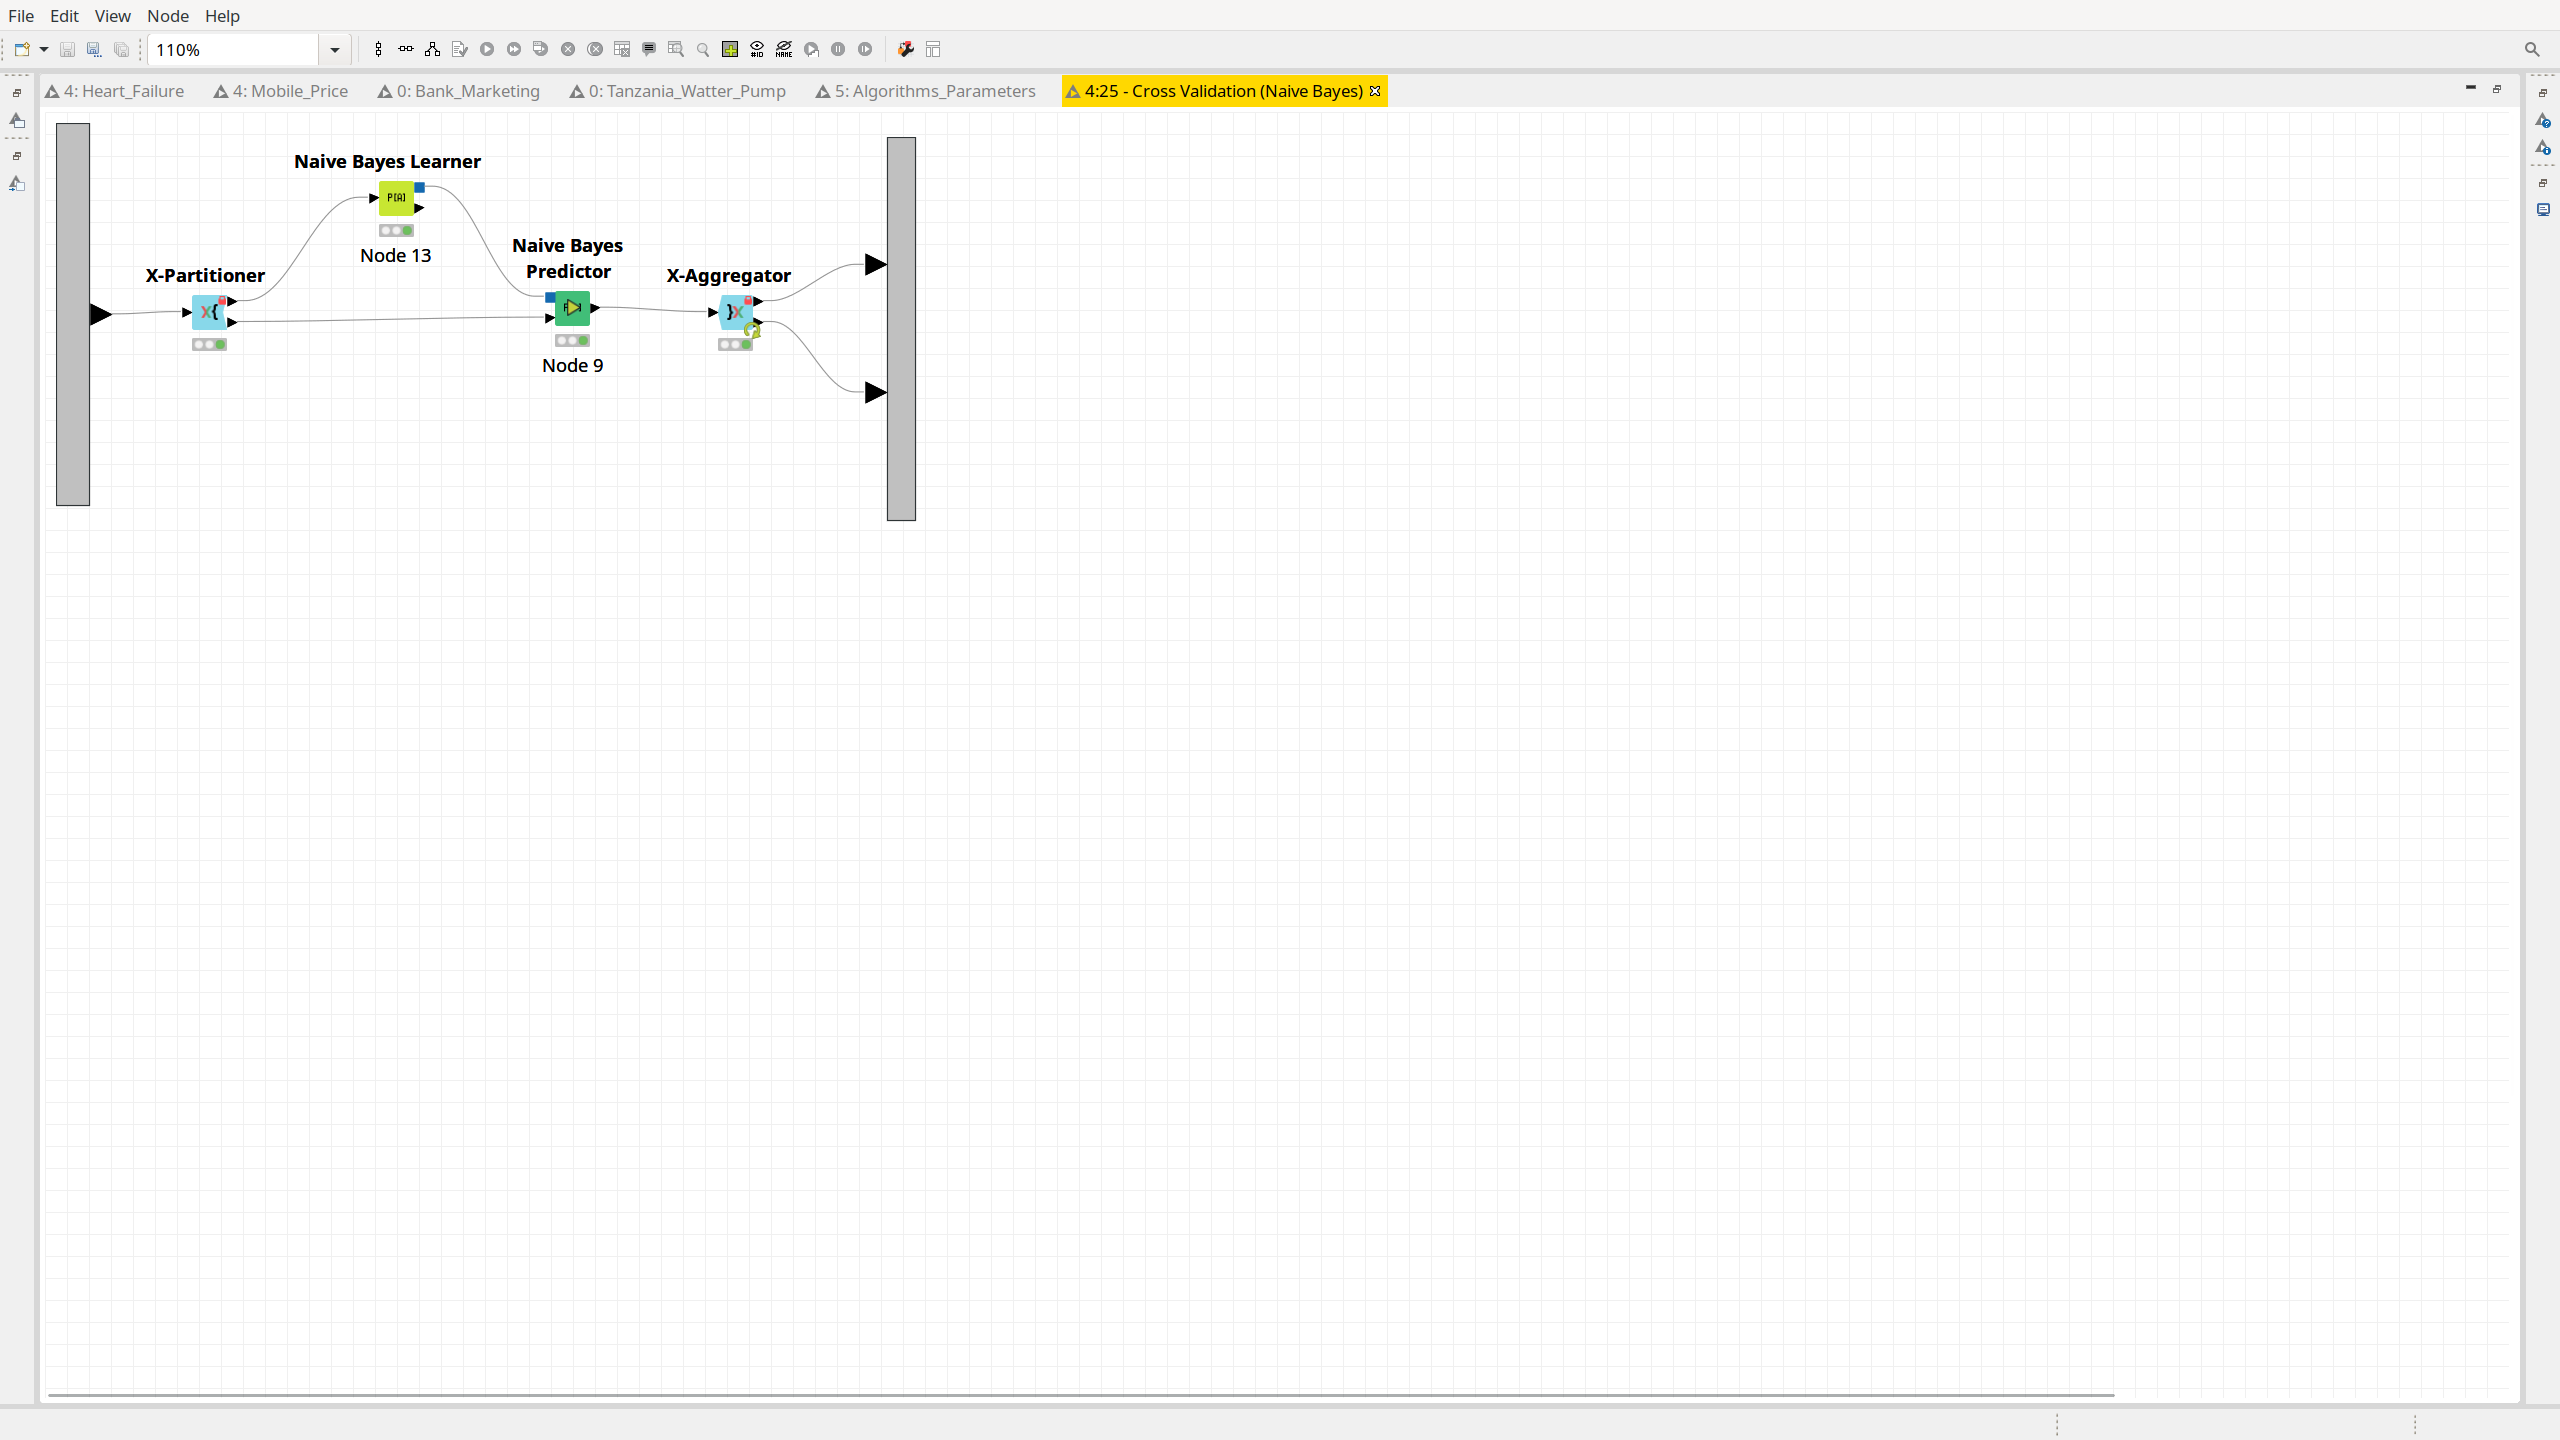
\includegraphics[width=1.0\textwidth]{\ipScreenshots/naive_bayes/nb.png}
\end{figure}

\begin{figure}[h!]
	\centering
	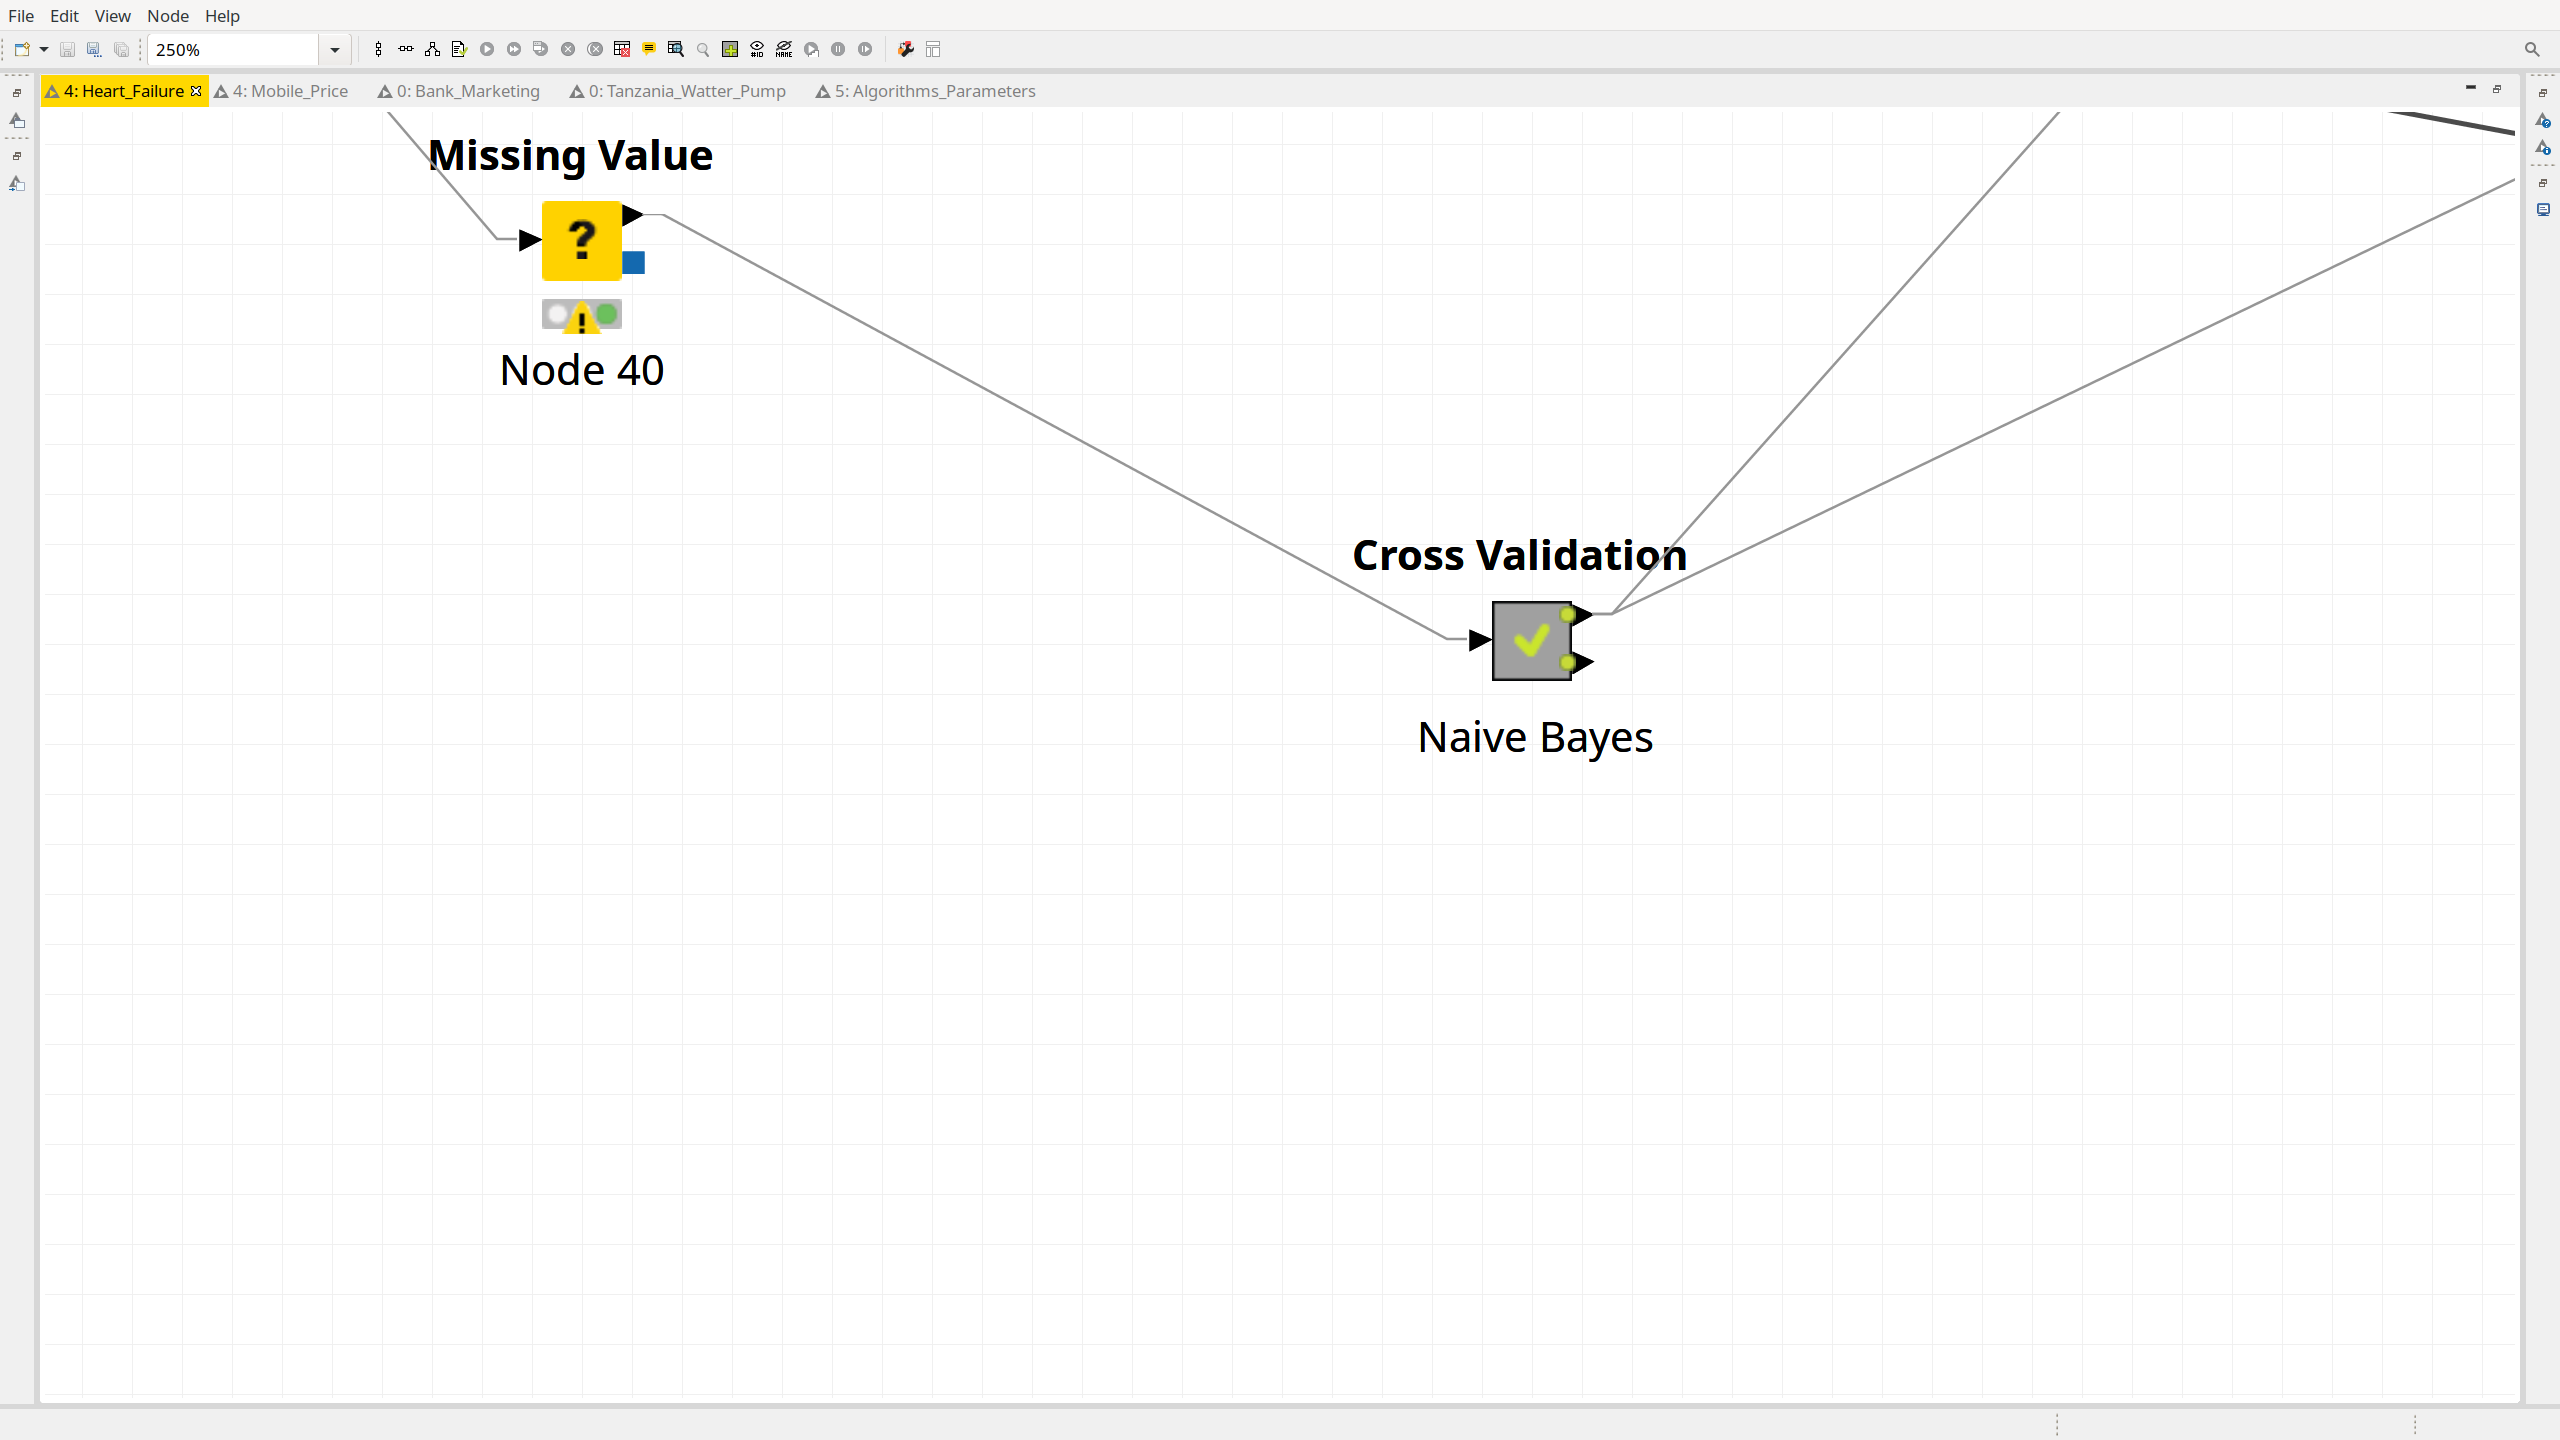
\includegraphics[width=1.0\textwidth]{\ipScreenshots/naive_bayes/pre_nb.png}
\end{figure}

\begin{center}
\resizebox{\textwidth}{!}{  %Usado para ajustar la tabla a los bordes del socumento
\pgfplotstabletypeset[
	col sep={comma},
	string type,
	column type=c,
	columns={Dataset,TP,FP,TN,FN,TPR,TNR,PPV,Accuracy,F-score,G-mean,AUC},
	every head row/.style={	before row={\rowcolor[gray]{0.9}}, after row=\hline,},
	% every last row/.style={ after row=\bottomrule},
	columns/Dataset/.style = {column type=l|},
	columns/TP/.style = {dec sep align},
	columns/FP/.style = {dec sep align},
	columns/TN/.style = {dec sep align},
	columns/FN/.style = {dec sep align},
	columns/TPR/.style = {precision = 4,fixed zerofill=true, dec sep align},
	columns/TNR/.style = {precision = 4,fixed zerofill=true, dec sep align},
	columns/PPV/.style = {precision = 4,fixed zerofill=true, dec sep align},
	columns/Accuracy/.style = {precision = 4,fixed zerofill=true, dec sep align},
	columns/F-score/.style = {precision = 4,fixed zerofill=true, dec sep align},
	columns/G-mean/.style = {precision = 4,fixed zerofill=true, dec sep align},
	columns/AUC/.style = {precision = 4,fixed zerofill=true, dec sep align},
]{Cuerpo/\ipAlgorithmsResults/Naive Bayes_Results.csv}
}
\end{center}


\clearpage
\subsection{Redes Neuronales}

\begin{figure}[h!]
	\centering
	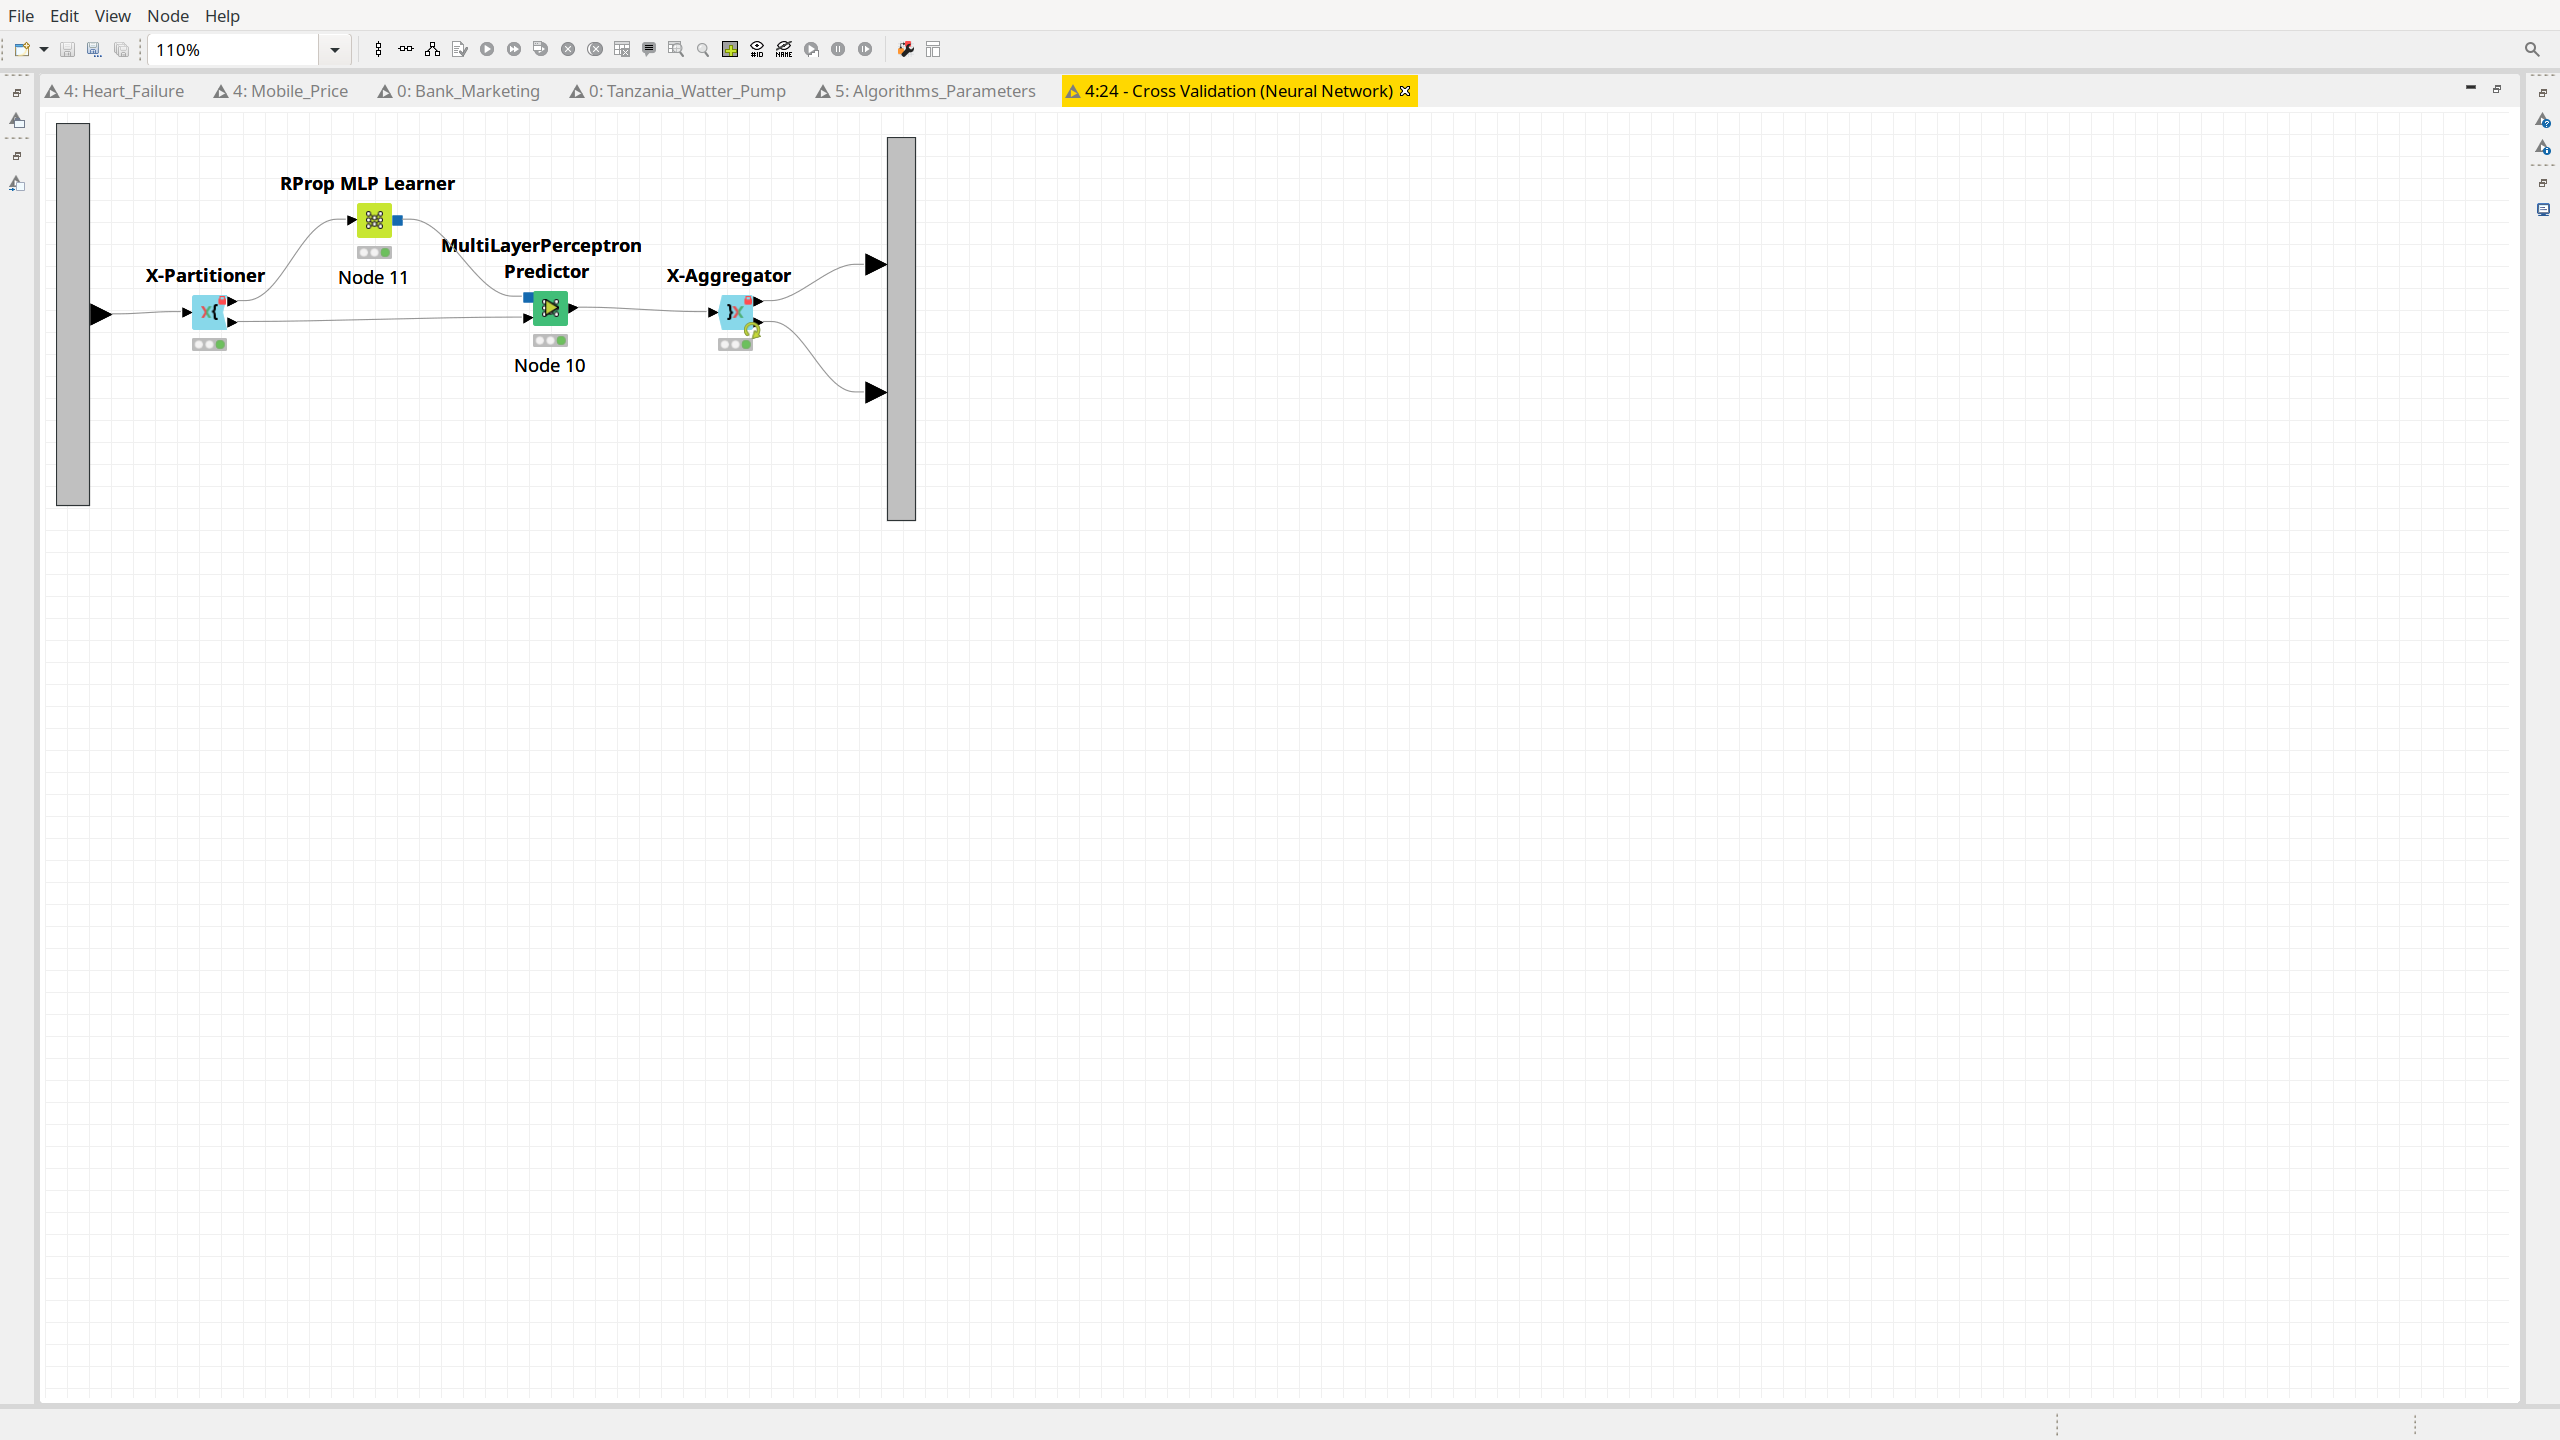
\includegraphics[width=1.0\textwidth]{\ipScreenshots/neural_network/ann.png}
\end{figure}

\begin{figure}[h!]
	\centering
	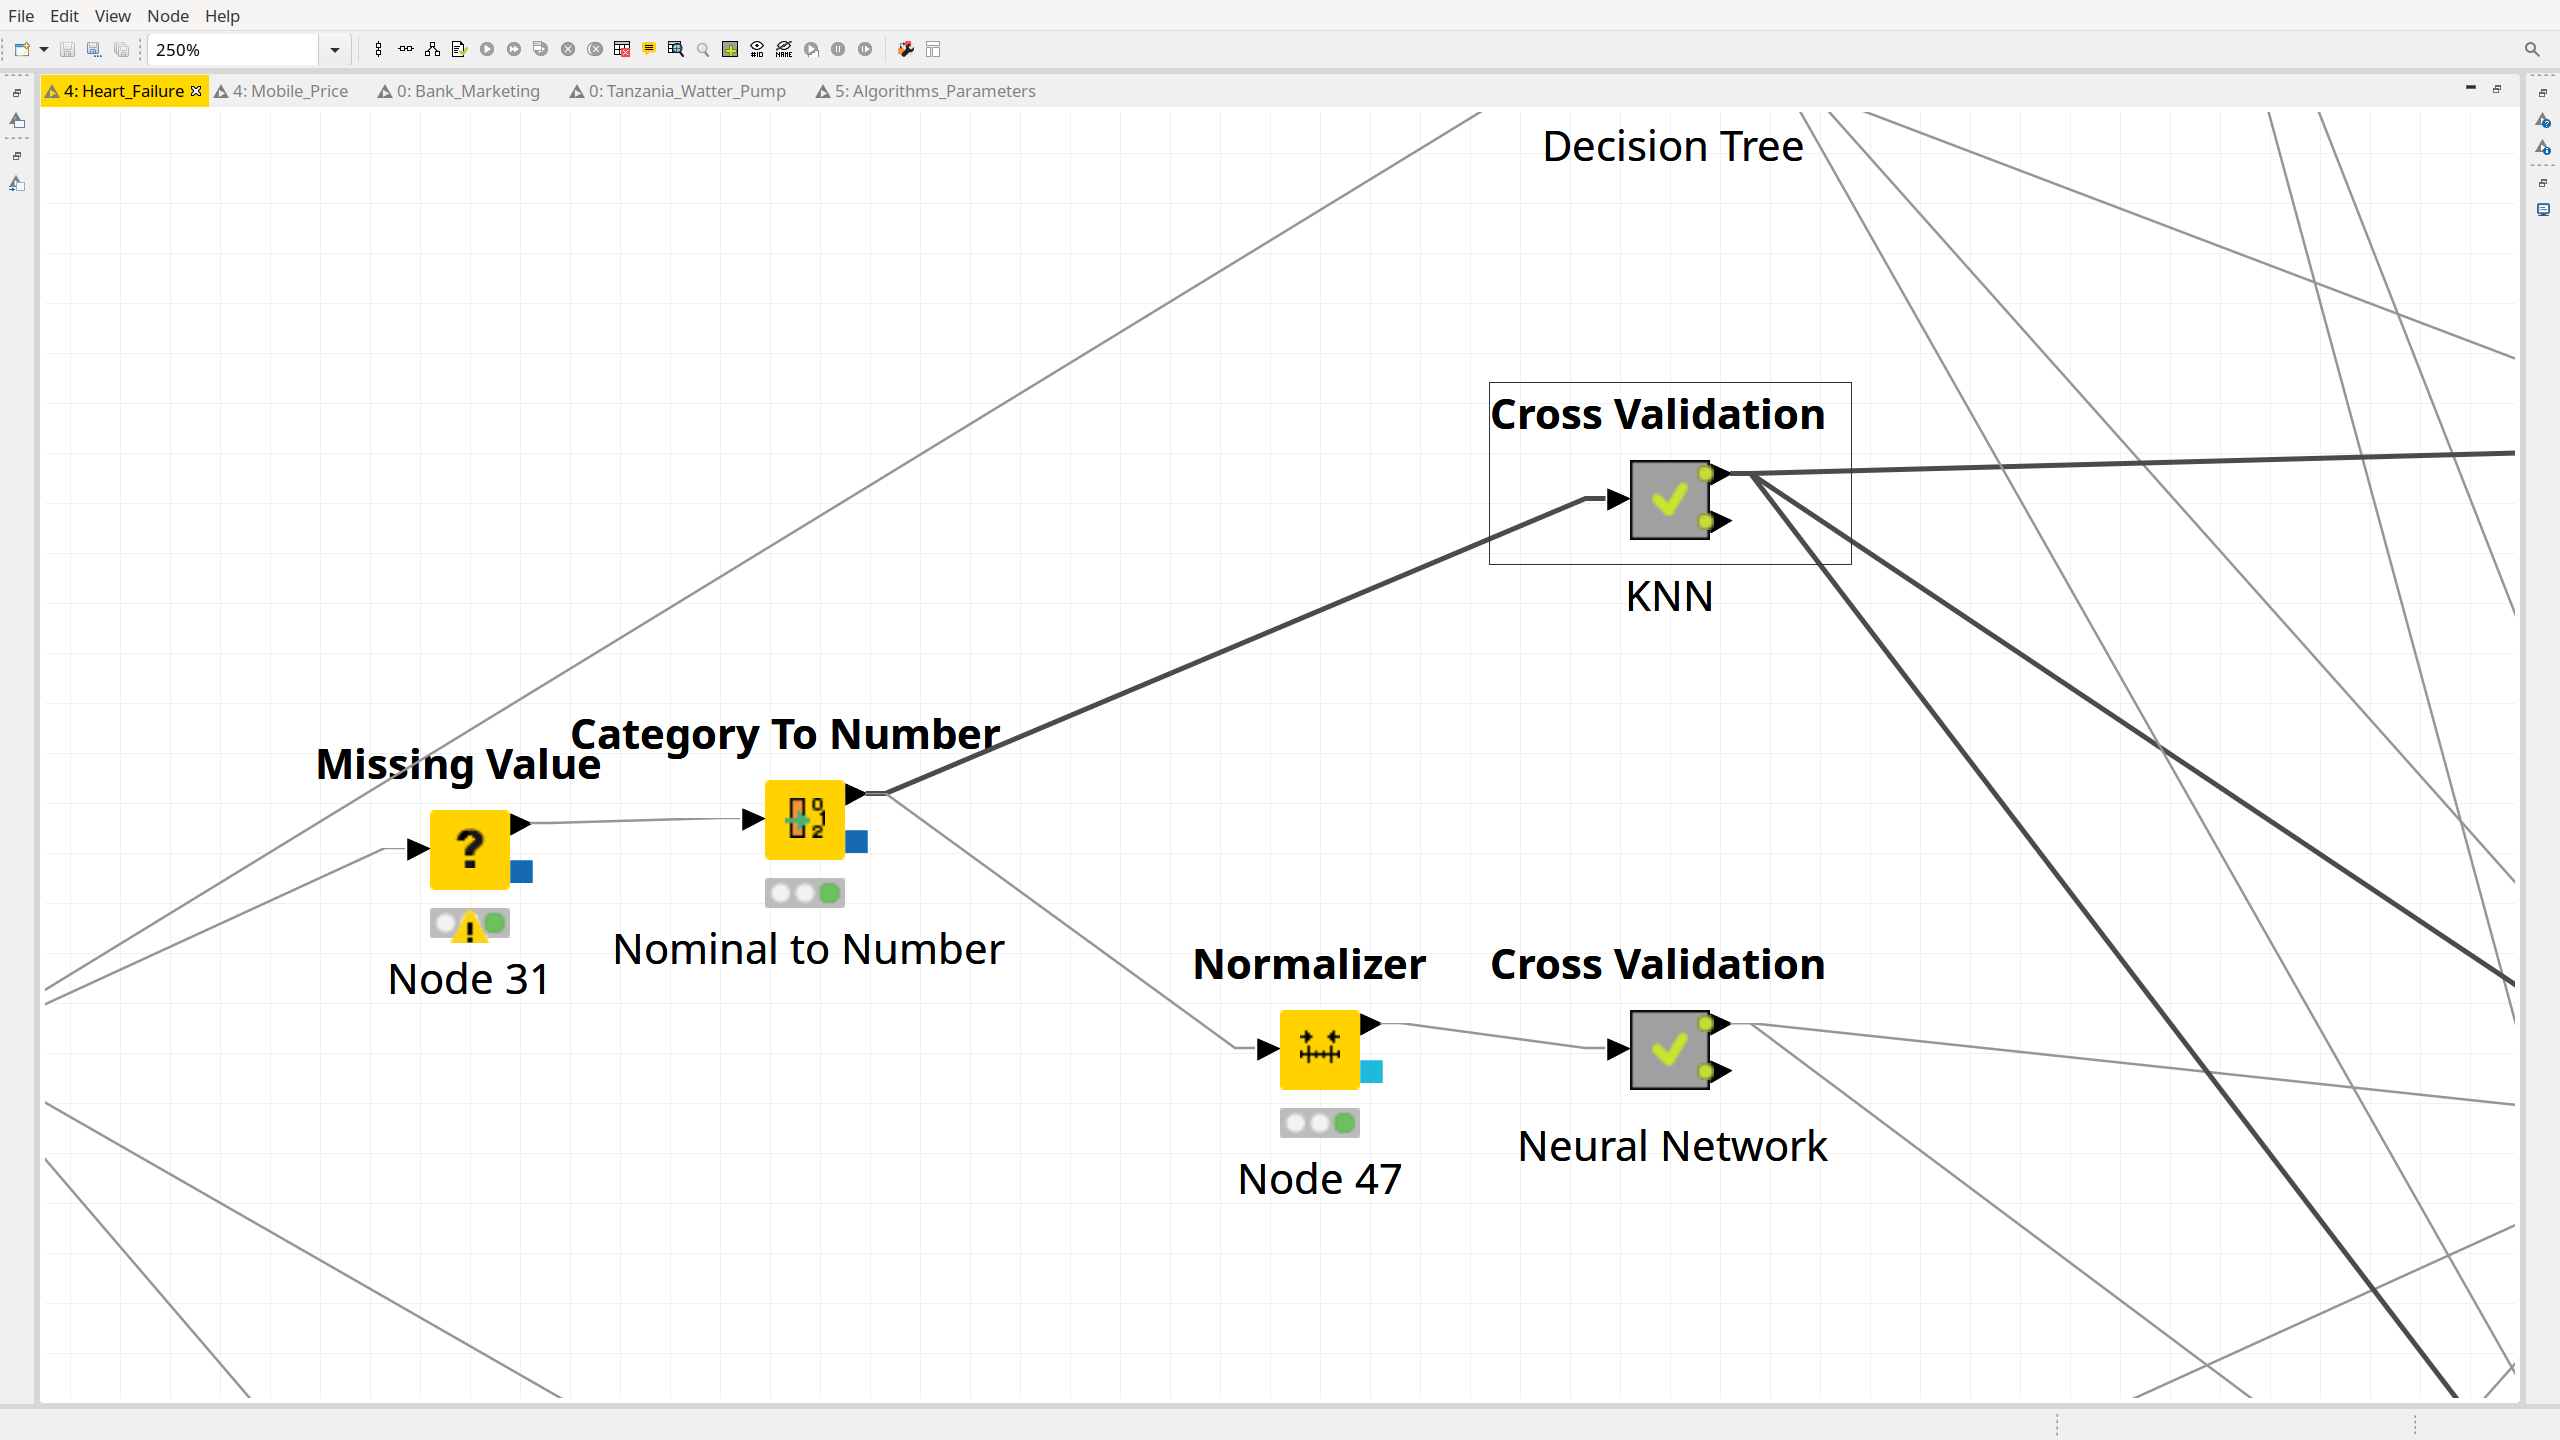
\includegraphics[width=1.0\textwidth]{\ipScreenshots/neural_network/pre_ann.png}
\end{figure}

\begin{center}
\resizebox{\textwidth}{!}{  %Usado para ajustar la tabla a los bordes del socumento
\pgfplotstabletypeset[
	col sep={comma},
	string type,
	column type=c,
	columns={Dataset,TP,FP,TN,FN,TPR,TNR,PPV,Accuracy,F-score,G-mean,AUC},
	every head row/.style={	before row={\rowcolor[gray]{0.9}}, after row=\hline,},
	%every last row/.style={ after row=\bottomrule},
	columns/Dataset/.style = {column type=l|},
	columns/TP/.style = {dec sep align},
	columns/FP/.style = {dec sep align},
	columns/TN/.style = {dec sep align},
	columns/FN/.style = {dec sep align},
	columns/TPR/.style = {precision = 4,fixed zerofill=true, dec sep align},
	columns/TNR/.style = {precision = 4,fixed zerofill=true, dec sep align},
	columns/PPV/.style = {precision = 4,fixed zerofill=true, dec sep align},
	columns/Accuracy/.style = {precision = 4,fixed zerofill=true, dec sep align},
	columns/F-score/.style = {precision = 4,fixed zerofill=true, dec sep align},
	columns/G-mean/.style = {precision = 4,fixed zerofill=true, dec sep align},
	columns/AUC/.style = {precision = 4,fixed zerofill=true, dec sep align},
]{Cuerpo/\ipAlgorithmsResults/Neural Network_Results.csv}
}
\end{center}


\clearpage
\subsection{Random Forest}

\begin{figure}[h!]
	\centering
	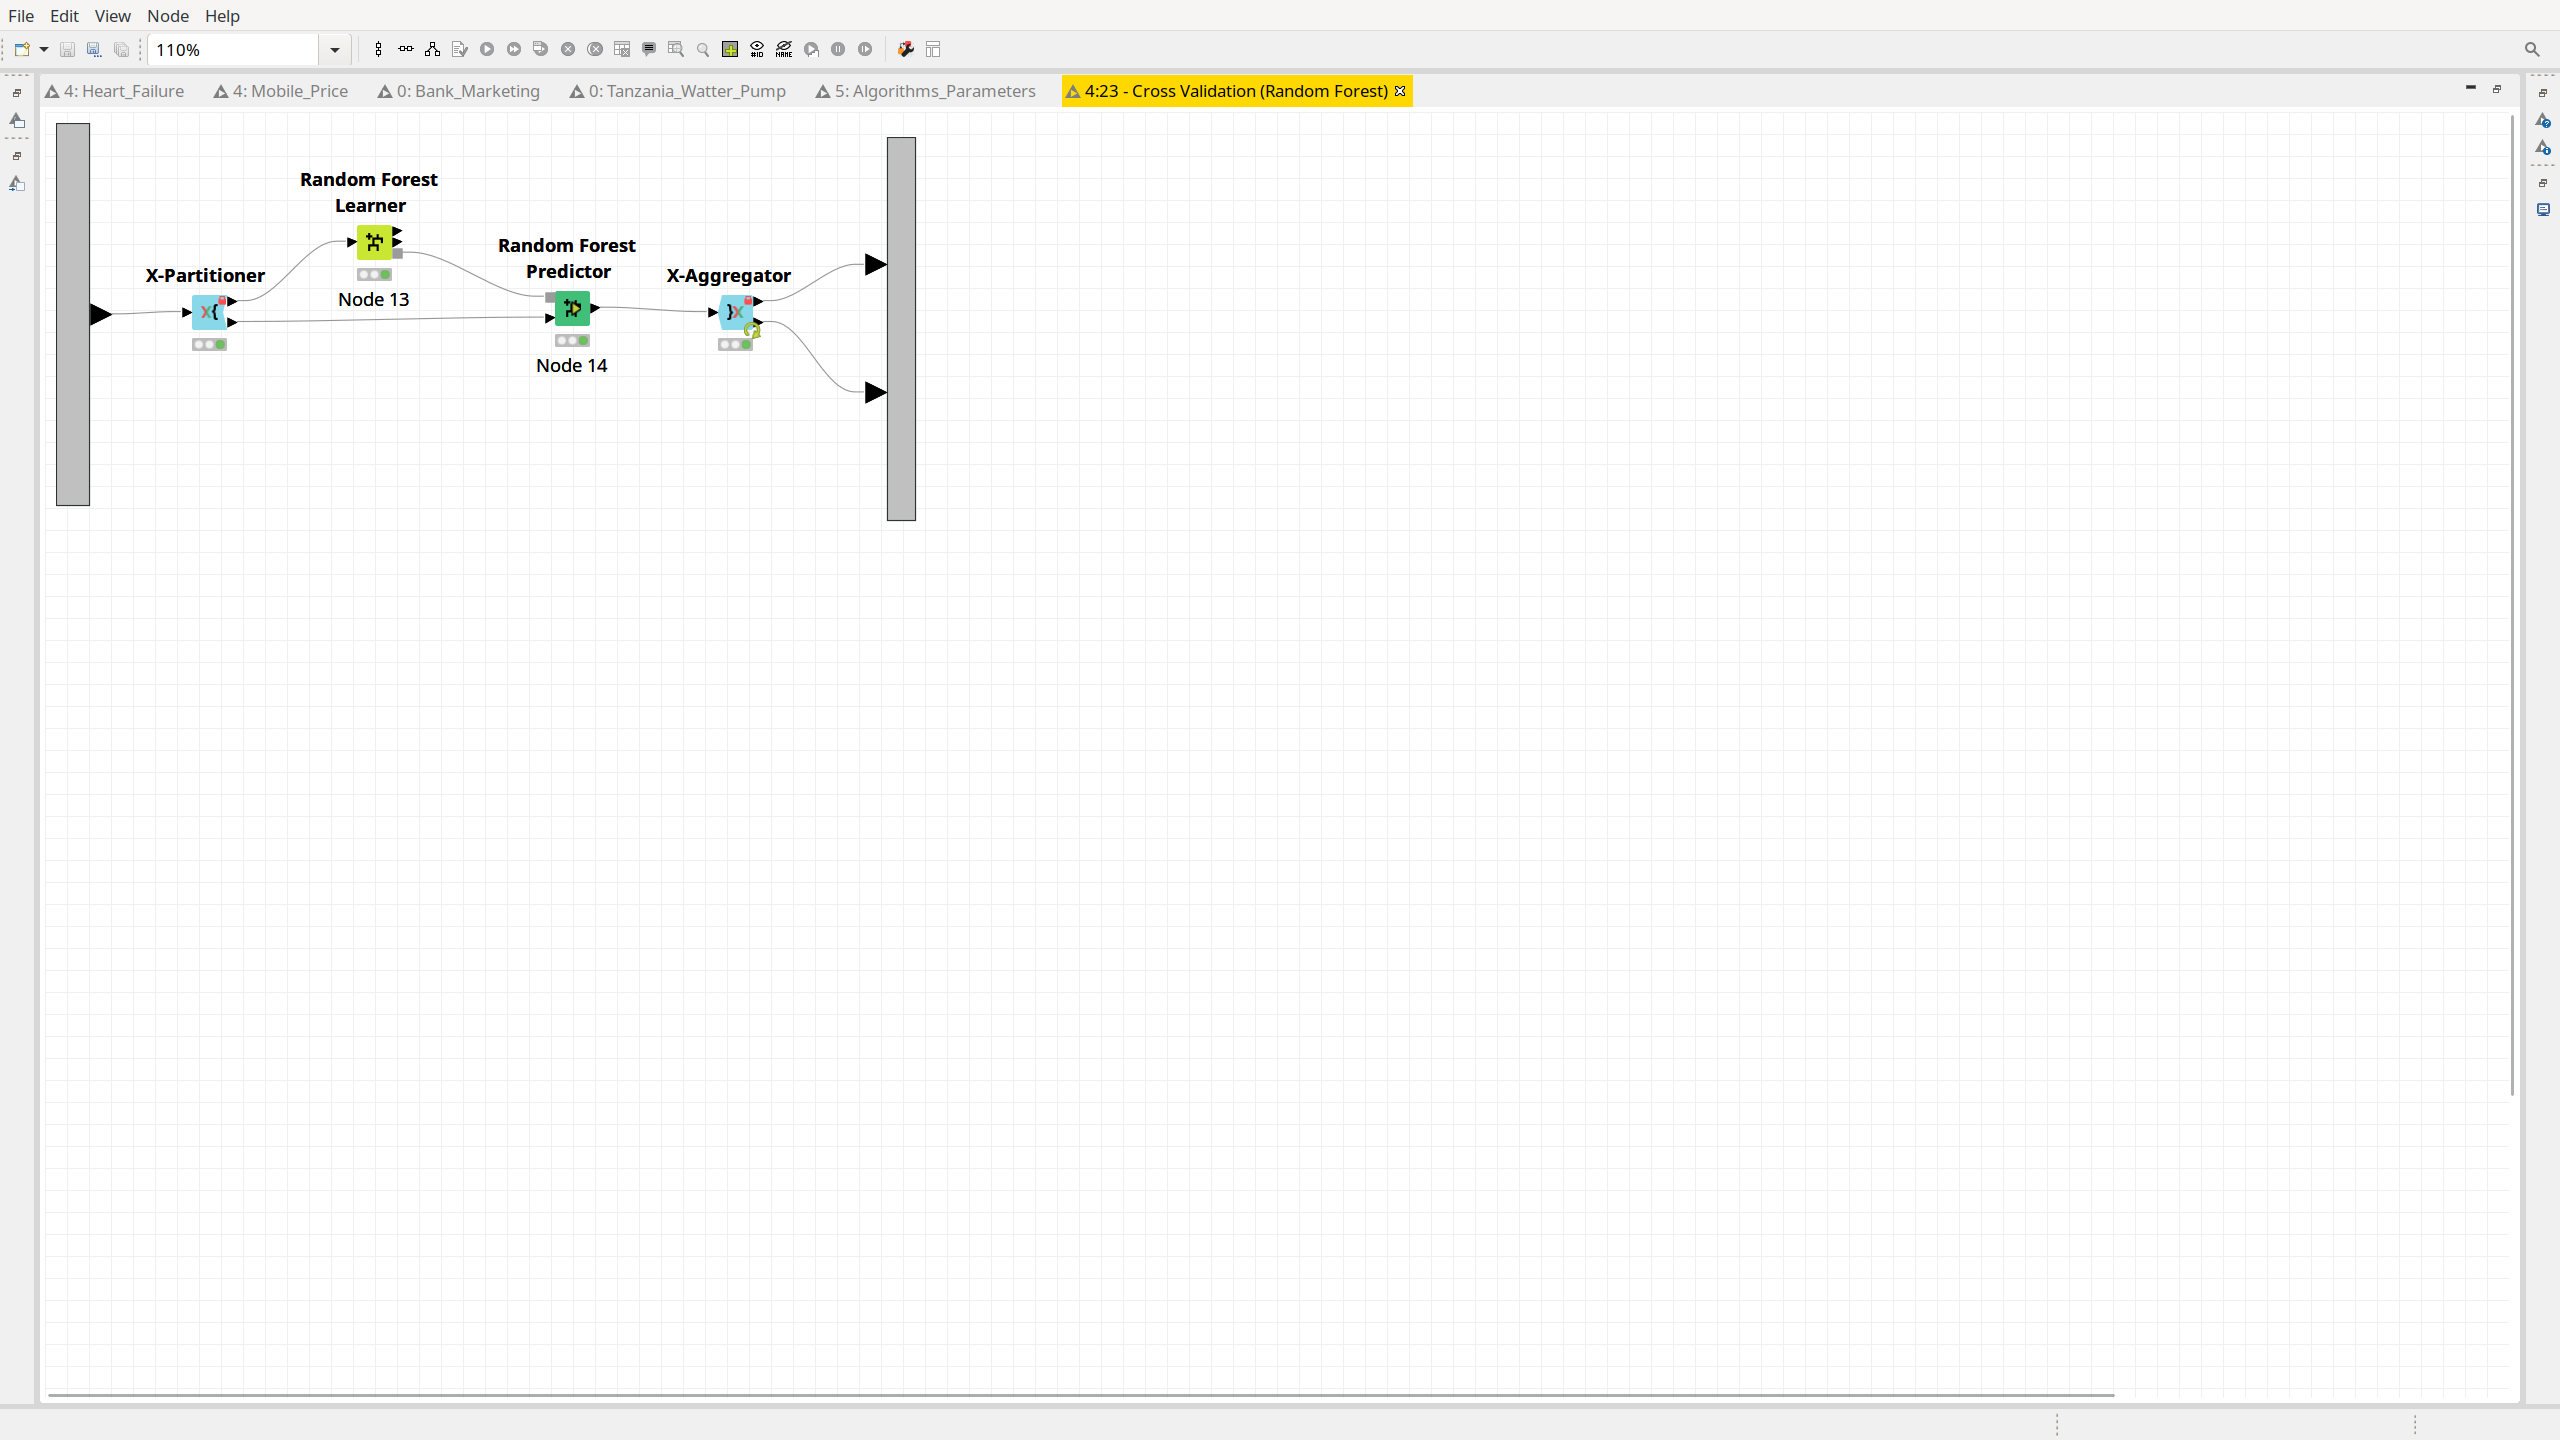
\includegraphics[width=1.0\textwidth]{\ipScreenshots/random_forest/rf.png}
\end{figure}

\begin{figure}[h!]
	\centering
	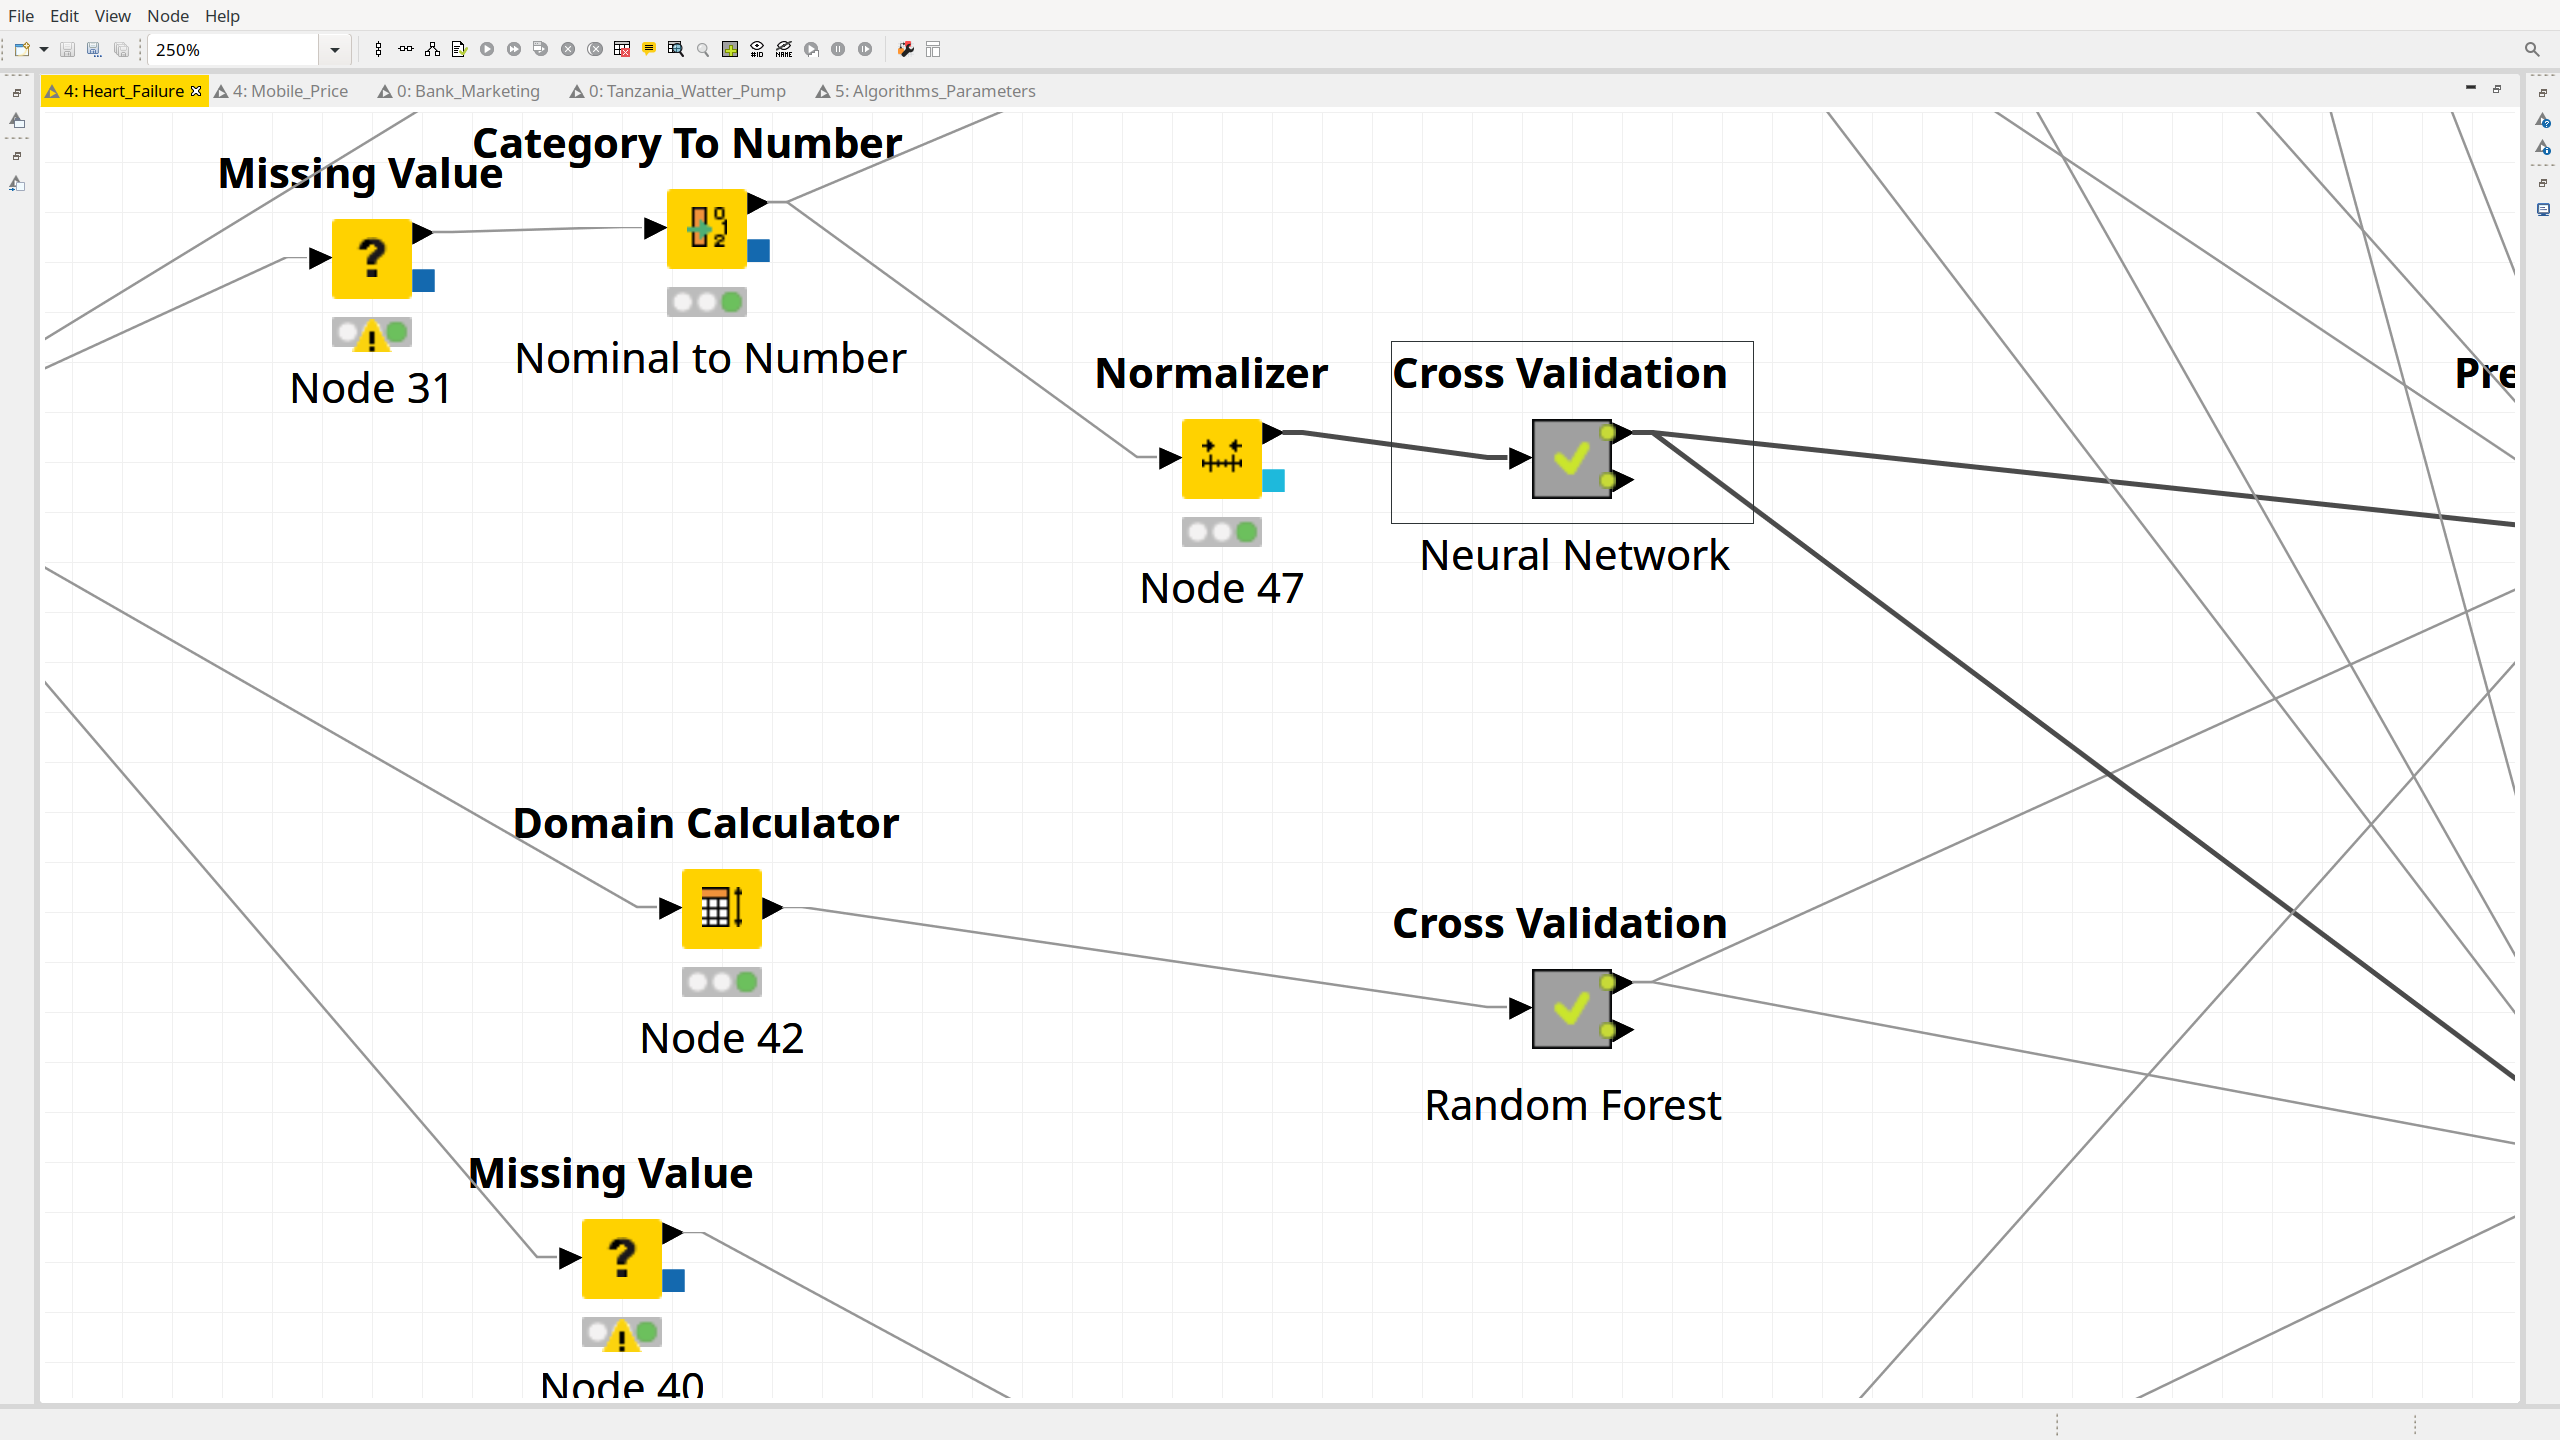
\includegraphics[width=1.0\textwidth]{\ipScreenshots/random_forest/pre_rf.png}
\end{figure}

\begin{center}
\resizebox{\textwidth}{!}{  %Usado para ajustar la tabla a los bordes del socumento
\pgfplotstabletypeset[
	col sep={comma},
	string type,
	column type=c,
	columns={Dataset,TP,FP,TN,FN,TPR,TNR,PPV,Accuracy,F-score,G-mean,AUC},
	every head row/.style={	before row={\rowcolor[gray]{0.9}}, after row=\hline,},
	%every last row/.style={ after row=\bottomrule},
	columns/Dataset/.style = {column type=l|},
	columns/TP/.style = {dec sep align},
	columns/FP/.style = {dec sep align},
	columns/TN/.style = {dec sep align},
	columns/FN/.style = {dec sep align},
	columns/TPR/.style = {precision = 4,fixed zerofill=true, dec sep align},
	columns/TNR/.style = {precision = 4,fixed zerofill=true, dec sep align},
	columns/PPV/.style = {precision = 4,fixed zerofill=true, dec sep align},
	columns/Accuracy/.style = {precision = 4,fixed zerofill=true, dec sep align},
	columns/F-score/.style = {precision = 4,fixed zerofill=true, dec sep align},
	columns/G-mean/.style = {precision = 4,fixed zerofill=true, dec sep align},
	columns/AUC/.style = {precision = 4,fixed zerofill=true, dec sep align},
]{Cuerpo/\ipAlgorithmsResults/Random Forest_Results.csv}
}
\end{center}





\clearpage
\section{Análisis de los Resultados}

\subsection{Heart Failure Prediction}

\begin{figure}[h!]
	\centering
	\includesvg[width=.8\textwidth]{\ipHeartFailure/hf_roc.svg}
	\caption{Nodo \texttt{Heart Failure Prediction Roc Curve}}
\end{figure} 

\begin{center}
\vspace{1.5em}
\resizebox{\textwidth}{!}{  %Usado para ajustar la tabla a los bordes del socumento
\pgfplotstabletypeset[
	col sep={comma},
	string type,
	column type=c,
	columns={Algorithms,TPR,TNR,PPV,Accuracy,F-score,G-mean,AUC},
	every head row/.style={	before row={\rowcolor[gray]{0.9}}, after row=\hline,},
	%every last row/.style={ after row=\bottomrule},
	columns/Algorithms/.style	={column type=l|},
	columns/TPR/.style = {precision = 4,fixed zerofill=true, dec sep align},
	columns/TNR/.style = {precision = 4,fixed zerofill=true, dec sep align},
	columns/PPV/.style = {precision = 4,fixed zerofill=true, dec sep align},
	columns/Accuracy/.style = {precision = 4,fixed zerofill=true, dec sep align},
	columns/F-score/.style = {precision = 4,fixed zerofill=true, dec sep align},
	columns/G-mean/.style = {precision = 4,fixed zerofill=true, dec sep align},
	columns/AUC/.style = {precision = 4,fixed zerofill=true, dec sep align},
]{Cuerpo/\ipHeartFailure/results.csv}
}

\vspace{1.5em}
\resizebox{\textwidth}{!}{  %Usado para ajustar la tabla a los bordes del socumento
\pgfplotstabletypeset[
	col sep={comma},
	string type,
	column type=c,
	columns={Algorithms,Tree Size,Training Size,Max. Values,N. Iters,N. Layers,N. Neurons,N. Trees},
	every head row/.style={	before row={\rowcolor[gray]{0.9}}, after row=\hline,},
	every nth row={1}{before row=\hline},
	columns/Algorithms/.style = {column type=l|},
	columns/Tree Size/.style = {column type=c},
	columns/Training Size/.style = {column type=c},
	columns/Max. Values/.style = {column type=c},
	columns/N. Iters/.style = {column type=c},
	columns/N. Layers/.style = {column type=c},
	columns/N. Neurons/.style = {column type=c},
	columns/N. Trees/.style = {column type=c},
]{Cuerpo/\ipHeartFailure/results.csv}
}
\end{center}

\vspace{1.5em}
En el primero de los datasets los resultados de los algoritmos son buenos en general a escepción de KNN que queda muy rezagado. Los algoritmos que mejor tasa de acierto tienen sobre la clase positiva son NB y RF. ANN y RF son los que tienen mejor PPV. Con respecto al resto de indecadores ANN es el vencedor en la tasa de acierto sobre la clase negativa y NB y ANN se reparten el resto muy cercanos el uno del otro.

El problema consiste en predecir si un paciente tiene una enfermedad de cardiovascular. Por lo tanto, la tasa de acierto sobre la clase negativa es el indicador más relevante puesto que un falso positivo no tiene mayor repercusión que la que suponga realizar un conjunto de pruebas médicas mientras que un falso negativo puede tener consecuencias fatales. El coste del error de predición de la clase negativa es mucho mayor. Por tanto, renta ser conservativo en ese sentido. El indicador que mide el acierto en la clase negativa es TNR y es, por lo tanto el más adevuado para evaluar los clasificadores en este problema.

Por ser la especificidad el indicador más relevante los mejores modelos son NB y RF que obtienen exactamente la misma puntuación. Para escoger entre estos dos modelos lo mejor es utilizar el resto de indicadores. Por ser RF superior en el resto de indicadores este es el mejor modelo.


\subsection{Mobile Price Classification}

\begin{figure}[h!]
	\centering
	\includesvg[width=.8\textwidth]{\ipMobilePrice/mp_roc.svg}
	\caption{Nodo \texttt{Mobile Price Classification Roc Curve}}
\end{figure}

\begin{center}
\vspace{1.5em}
\resizebox{\textwidth}{!}{  %Usado para ajustar la tabla a los bordes del socumento
\pgfplotstabletypeset[
	col sep={comma},
	string type,
	column type=c,
	columns={Algorithms,TPR,TNR,PPV,Accuracy,F-score,G-mean,AUC},
	every head row/.style={	before row={\rowcolor[gray]{0.9}}, after row=\hline,},
	%every last row/.style={ after row=\bottomrule},
	columns/Algorithms/.style = {column type=l|},
	columns/TPR/.style = {precision = 4,fixed zerofill=true, dec sep align},
	columns/TNR/.style = {precision = 4,fixed zerofill=true, dec sep align},
	columns/PPV/.style = {precision = 4,fixed zerofill=true, dec sep align},
	columns/Accuracy/.style = {precision = 4,fixed zerofill=true, dec sep align},
	columns/F-score/.style = {precision = 4,fixed zerofill=true, dec sep align},
	columns/G-mean/.style = {precision = 4,fixed zerofill=true, dec sep align},
	columns/AUC/.style = {precision = 4,fixed zerofill=true, dec sep align},
]{Cuerpo/\ipMobilePrice/results.csv}
}

\vspace{1.5em}
\resizebox{\textwidth}{!}{  %Usado para ajustar la tabla a los bordes del socumento
\pgfplotstabletypeset[
	col sep={comma},
	string type,
	column type=c,
	columns={Algorithms,Tree Size,Training Size,Max. Values,N. Iters,N. Layers,N. Neurons,N. Trees},
	every head row/.style={	before row={\rowcolor[gray]{0.9}}, after row=\hline,},
	every nth row={1}{before row=\hline},
	columns/Algorithms/.style = {column type=l|},
	columns/Tree Size/.style = {column type=c},
	columns/Training Size/.style = {column type=c},
	columns/Max. Values/.style = {column type=c},
	columns/N. Iters/.style = {column type=c},
	columns/N. Layers/.style = {column type=c},
	columns/N. Neurons/.style = {column type=c},
	columns/N. Trees/.style = {column type=c},
]{Cuerpo/\ipMobilePrice/results.csv}
}
\end{center}

\vspace{1.5em}
En el segundo dataset todos los modelos obtienen resultados excelentes. Los algoritmos con mayor TPR son KNN y RF mientras que en que vuelve a tener mayor TNR es ANN. El resto de los indicadores están repartidos entre estos tres algoritmos. En particular ANN es vencedora en G-mean y AUC.

El problema consiste en predecir el rango de precio de dispositivos moviles. En este problema hay cuatro clases que están perfectamente balanceadas y todas ellas son igual de relavantes en el sentido de que el peso del error es igual para todas ellas. El mejor clasificador será, por lo tanto, aquel con mayor puntuación en indicadores que midan el acierto en todas las clases como son F-score, G-mean y AUC. 

Como consecuencia el mejor de los algoritmos será ANN que es el mejor algoritmo estas tres métricas.
El segundo mejor clasificador sería, probablemente, RF.


\subsection{Bank Marketing}

\begin{figure}[h!]
	\centering
	\includesvg[width=.8\textwidth]{\ipBankMarketing/bm_roc.svg}
	\caption{Nodo \texttt{Bank Marketing Roc Curve}}
\end{figure}

\begin{center}
\vspace{1.5em}
\resizebox{\textwidth}{!}{  %Usado para ajustar la tabla a los bordes del socumento
\pgfplotstabletypeset[
	col sep={comma},
	string type,
	column type=c,
	columns={Algorithms,TPR,TNR,PPV,Accuracy,F-score,G-mean,AUC},
	every head row/.style={	before row={\rowcolor[gray]{0.9}}, after row=\hline,},
	%every last row/.style={ after row=\bottomrule},
	columns/Algorithms/.style	={column type=l|},
	columns/TPR/.style = {precision = 4,fixed zerofill=true, dec sep align},
	columns/TNR/.style = {precision = 4,fixed zerofill=true, dec sep align},
	columns/PPV/.style = {precision = 4,fixed zerofill=true, dec sep align},
	columns/Accuracy/.style = {precision = 4,fixed zerofill=true, dec sep align},
	columns/F-score/.style = {precision = 4,fixed zerofill=true, dec sep align},
	columns/G-mean/.style = {precision = 4,fixed zerofill=true, dec sep align},
	columns/AUC/.style = {precision = 4,fixed zerofill=true, dec sep align},
]{Cuerpo/\ipBankMarketing/results.csv}
}

\vspace{1.5em}
\resizebox{\textwidth}{!}{  %Usado para ajustar la tabla a los bordes del socumento
\pgfplotstabletypeset[
	col sep={comma},
	string type,
	column type=c,
	columns={Algorithms,Tree Size,Training Size,Max. Values,N. Iters,N. Layers,N. Neurons,N. Trees},
	every head row/.style={	before row={\rowcolor[gray]{0.9}}, after row=\hline,},
	every nth row={1}{before row=\hline},
	columns/Algorithms/.style = {column type=l|},
	columns/Tree Size/.style = {column type=c},
	columns/Training Size/.style = {column type=c},
	columns/Max. Values/.style = {column type=c},
	columns/N. Iters/.style = {column type=c},
	columns/N. Layers/.style = {column type=c},
	columns/N. Neurons/.style = {column type=c},
	columns/N. Trees/.style = {column type=c},
]{Cuerpo/\ipBankMarketing/results.csv}
}
\end{center}

\vspace{1.5em}
En el tercer problema lor resultados son en general buenos pero hay diferencias notables entre los algoritmos. RF es el clasificador con mayor acierto en la clase positiva mientras que NB es el que tiene mayor acierto en la clase negativa. En accuracy y F-score RF es el clasificador con mejor puntuación así como el que mayor área deja bajo la curva ROC siendo DT el que menos.

El problema consistía en predecir si un cliente se abonaría a un depósito ofrecido por su banco. Como ya se comentó en la introducción las clases están fuertemente desbalanceadas cen más de un 88\% de los clientes en la clase negativa. Es por lo tanto necesario utilizar medidas que contemplen dicho desbalanceo a la hora de intentar seleccionar el mejor clasificador. El indicador F-score es perfecto para esto puesto que mide un compromiso entre \texttt{Precision} y \texttt{Recall} quedando gravemente perjudicada si alguna de las dos baja puestos que utiliza la media harmónica.

Por lo tanto el mejor clasificador es ANN que supera a todos los clasificadores en F-score por una pequeña diferencia a excepción de RF que lo sigue de cerca. En la curva ROC se observa que DT esta muy cercano a la diagonal. Esto es mucho peor que una curva que progresa cercana al borde de la grafica e indica que al comienzo el clasificador tiene la misma bondad que el clasificador aleatorio.


\subsection{Tanzania Watter Pump}
\label{sec:tanzania-results}

\begin{figure}[h!]
	\centering
	\includesvg[width=.8\textwidth]{\ipTanzania/twp_roc.svg}
	\caption{Nodo \texttt{Tanzania Watter Pump Roc Curve}}
\end{figure}

\vspace{1.5em}

\begin{center}
\resizebox{\textwidth}{!}{  %Usado para ajustar la tabla a los bordes del socumento
\pgfplotstabletypeset[
	col sep={comma},
	string type,
	column type=c,
	columns={Algorithms,TPR,TNR,PPV,Accuracy,F-score,G-mean,AUC},
	every head row/.style={	before row={\rowcolor[gray]{0.9}}, after row=\hline,},
	%every last row/.style={ after row=\bottomrule},
	columns/Algorithms/.style	={column type=l|},
	columns/TPR/.style = {precision = 4,fixed zerofill=true, dec sep align},
	columns/TNR/.style = {precision = 4,fixed zerofill=true, dec sep align},
	columns/PPV/.style = {precision = 4,fixed zerofill=true, dec sep align},
	columns/Accuracy/.style = {precision = 4,fixed zerofill=true, dec sep align},
	columns/F-score/.style = {precision = 4,fixed zerofill=true, dec sep align},
	columns/G-mean/.style = {precision = 4,fixed zerofill=true, dec sep align},
	columns/AUC/.style = {precision = 4,fixed zerofill=true, dec sep align},
]{Cuerpo/\ipTanzania/results.csv}
}

\vspace{1.5em}
\resizebox{\textwidth}{!}{  %Usado para ajustar la tabla a los bordes del socumento
\pgfplotstabletypeset[
	col sep={comma},
	string type,
	column type=c,
	columns={Algorithms,Tree Size,Training Size,Max. Values,N. Iters,N. Layers,N. Neurons,N. Trees},
	every head row/.style={	before row={\rowcolor[gray]{0.9}}, after row=\hline,},
	every nth row={1}{before row=\hline},
	columns/Algorithms/.style = {column type=l|},
	columns/Tree Size/.style = {column type=c},
	columns/Training Size/.style = {column type=c},
	columns/Max. Values/.style = {column type=c},
	columns/N. Iters/.style = {column type=c},
	columns/N. Layers/.style = {column type=c},
	columns/N. Neurons/.style = {column type=c},
	columns/N. Trees/.style = {column type=c},
]{Cuerpo/\ipTanzania/results.csv}
}
\end{center}

\vspace{1.5em}
En el último problema todos los algoritmos obtienen buenos resultados salvo KNN. RF es superior en la mayoria de las métricas seguido por DT siedo superado sólo en TNR y PPV por este último.

El problema consiste en predecir el estado actual de una bomba de agua. En este problema es mucho más relevante el acierto en la clase funcional, esto es, la clase positiva puesto que los falsos positivo implica la falta de agua en una aldea debido a que una bomba averiada se ha clasificado como operativa. Por lo tanto el indicador más relevante a la hora de escoger un clasificador será TPR que indica precisamente el acierto en la clase positiva, en concreto indica que proporción de los positivos predichos son verdaderamente positivos.

Por lo tanto el clasificador más indicado para este problema es RF que tiene una puntuación TPR considerablemente mayor que el resto de modelos.



\subsection{Consideraciones Generales}
\label{sec:general-considerations}
Con respecto a DT, su comportamiento es mediocre en \textit{Mobile Price Classification} y en \textit{Tanzania Watter Pump} y malo en \textit{Bank Marketing}. Una primera hipótesis es pensar que la dificultad para tratar atributos numéricos continuos lo está lastrando pero esta hipótesis no se sostiene porque en \textit{Bank Marketing}, su peor dataset, la inmensa mayoría de atributos numéricos son discretos y en \textit{Tanzania Watter Pump} ocurre igual siendo la mayor parte de los atributos discretos. Una segunta hipótesis puede ser que la dificultad del algoritmo de aprendizaje para tratar con valores perdidos pero nuevamente \textit{Bank Marketing} no presenta ninguno y \textit{Mobile Price Classification} tampoco. Otra posible hipótesis es que DT traza dominios rectangulares sobre el dominio de los atributos y puede ser que estos problemas no presenten esa topología. Por último la hipótesis quizás más fiable es que el desbalanceo tan grande de clases esté afectando los resultados del algoritmo de forma considerable.

Resalta la falta de competitividad de KNN en dos de los datasets: \textit{Heart Failure Prediction} y \textit{Tanzania Watter Pump} asi como su falta de competencia en \textit{Bank Marketing}. Los motivos son probablemente varios. Puesto que KNN sólo puede trabajar con atributos numericos es necesario transformar los atributos categoricos en numéricos. Knime realiza esta transformación asignando un entero consecutivo por cada categoría empezando en 0. Este procedimiento no es ideal puesto que induce un orden artificial en la variables y esto puede lastrar al algoritmo. Por lo tanto una primera hipótesis puede ser que el algoritmo se comportará peor en los datasets con mayor proporción de variables categóricas. Esta hipótesis es factible pero no es capaz de explicar el fenómeno por si sóla puesto que \textit{Tanzania Watter Pump} tiene una gran cantidad de atributos categóricos pero \textit{Bank Marketing} tiene una mayor proporción de atributos categóricos que \textit{Heart Failure Prediction} y sin embargo KNN se comporta mejor en \textit{Bank Marketing}. Otra posibilidad es que, al no estar los datos normalizados y siendo este un algoritmo que utiliza las distancias entre los datos, la distribución de los valores y los rangos de los atributos causen una posible complicación. Por último también es posible que el valor de el número de vecinos no esté correctamente ajustado y como consecuencia las clases no queden bien diferenciadas. Se experimentará con este parámetro en la sección de configuración para estudiar la vericidad de la hipótesis.

NB obtiene sus peores resultadoe en \textit{Bank Marketing} y en \textit{Tanzania Watter Pump}. La hipótesis de la independencia de las variable respecto a la clase puede no ser cierta en estos casos y además estar causando problemas en la clasificación.

RF se comporta especialmente bien. Es un algoritmo robusto frente a outliers y valores perdidos y especialmente estable y lo ha puesto de manifiesto. Si bien es cierto que su tiempo de cómputo es bastante superior al del resto de los algoritmos.

ANN se comporta muy bien en todos los datasets a excepción de \textit{Tanzania Watter Pump} donde obtiene resultados mediocres. Curiosamente \textit{Tanzania Watter Pump} es el dataset con mayor tamaño lo cual en teoría debería beneficiar a la red neuronal si bien se aprecia que sucede lo contrario. La explicación probablemente subyace en un sobreajuste. La red neuronal sobreaprende los patrones adaptándose a las idiosincracias de los datos y no es capaz de generalizar y por lo tanto se comporta muy mal ante la clasificación de nuevos datos. Una posibilidad para solucionar el problema podría ser utilizar algún tipo de regularización.
 



Problemas con mas variables numericas otros con mas variables categoricas puede afectar a los resultados.
Forma de la curva ROC de KNN y DT persistente en los problemas.




\section{Configuración de los Algoritmos}

Todas las medidas que aparecen a continuación pertenecen al dataset \textit{Tanzania Watter Pump}. Se ha decidido experimentar con los parámetros de los algoritmos sobre este dataset porque es el que tenía medidas más bajas en terminos generales. Además permite experimentar con los valores del número de vecinos en KNN que se ha comportado muy mal con el valor por defecto en este dataset. 

No se han modificado los parámetros de DT. El parámetro que varía para KNN es \texttt{Número de Vecinos} para NB es \texttt{Número de Valores por Atributo}, para ANN es \texttt{Número de Iteraciones} y para RF es \texttt{Número de Árboles}.


\clearpage
\subsection{Resultados}

\subsubsection{Primera Combinación}
El parámetro para KNN son 5 vecinos y para NB son 200 valores los valores del resto de atributos se muestran en la tabla.

\begin{figure}[h!]
	\centering
	\includesvg[width=.8\textwidth]{\ipParameters/roc1.svg}
\end{figure}

\vspace{1.0em}

\begin{center}
\resizebox{\textwidth}{!}{  %Usado para ajustar la tabla a los bordes del socumento
\pgfplotstabletypeset[
	col sep={comma},
	string type,
	column type=c,
	columns={Algorithms,TPR,TNR,PPV,Accuracy,F-score,G-mean,AUC},
	every head row/.style={	before row={\rowcolor[gray]{0.9}}, after row=\hline,},
	%every last row/.style={ after row=\bottomrule},
	columns/Algorithms/.style	={column type=l|},
	columns/TPR/.style = {precision = 4,fixed zerofill=true, dec sep align},
	columns/TNR/.style = {precision = 4,fixed zerofill=true, dec sep align},
	columns/PPV/.style = {precision = 4,fixed zerofill=true, dec sep align},
	columns/Accuracy/.style = {precision = 4,fixed zerofill=true, dec sep align},
	columns/F-score/.style = {precision = 4,fixed zerofill=true, dec sep align},
	columns/G-mean/.style = {precision = 4,fixed zerofill=true, dec sep align},
	columns/AUC/.style = {precision = 4,fixed zerofill=true, dec sep align},
]{Cuerpo/\ipParameters/results1.csv}
}

\vspace{1.5em}
\resizebox{\textwidth}{!}{  %Usado para ajustar la tabla a los bordes del socumento
\pgfplotstabletypeset[
	col sep={comma},
	string type,
	column type=c,
	columns={Algorithms,Tree Size,Training Size,Max. Values,N. Iters,N. Layers,N. Neurons,N. Trees},
	every head row/.style={	before row={\rowcolor[gray]{0.9}}, after row=\hline,},
	every nth row={1}{before row=\hline},
	columns/Algorithms/.style = {column type=l|},
	columns/Tree Size/.style = {column type=c},
	columns/Training Size/.style = {column type=c},
	columns/Max. Values/.style = {column type=c},
	columns/N. Iters/.style = {column type=c},
	columns/N. Layers/.style = {column type=c},
	columns/N. Neurons/.style = {column type=c},
	columns/N. Trees/.style = {column type=c},
]{Cuerpo/\ipParameters/results1.csv}
}
\end{center}


\clearpage
\subsubsection{Segunda Combinación}
El parámetro para KNN son 7 vecinos y para NB son 2000 valores los valores del resto de atributos se muestran en la tabla.

\begin{figure}[h!]
	\centering
	\includesvg[width=.8\textwidth]{\ipParameters/roc2.svg}
\end{figure}

\vspace{1.5em}

\begin{center}
\resizebox{\textwidth}{!}{  %Usado para ajustar la tabla a los bordes del socumento
\pgfplotstabletypeset[
	col sep={comma},
	string type,
	column type=c,
	columns={Algorithms,TPR,TNR,PPV,Accuracy,F-score,G-mean,AUC},
	every head row/.style={	before row={\rowcolor[gray]{0.9}}, after row=\hline,},
	%every last row/.style={ after row=\bottomrule},
	columns/Algorithms/.style	={column type=l|},
	columns/TPR/.style = {precision = 4,fixed zerofill=true, dec sep align},
	columns/TNR/.style = {precision = 4,fixed zerofill=true, dec sep align},
	columns/PPV/.style = {precision = 4,fixed zerofill=true, dec sep align},
	columns/Accuracy/.style = {precision = 4,fixed zerofill=true, dec sep align},
	columns/F-score/.style = {precision = 4,fixed zerofill=true, dec sep align},
	columns/G-mean/.style = {precision = 4,fixed zerofill=true, dec sep align},
	columns/AUC/.style = {precision = 4,fixed zerofill=true, dec sep align},
]{Cuerpo/\ipParameters/results2.csv}
}

\vspace{1.5em}
\resizebox{\textwidth}{!}{  %Usado para ajustar la tabla a los bordes del socumento
\pgfplotstabletypeset[
	col sep={comma},
	string type,
	column type=c,
	columns={Algorithms,Tree Size,Training Size,Max. Values,N. Iters,N. Layers,N. Neurons,N. Trees},
	every head row/.style={	before row={\rowcolor[gray]{0.9}}, after row=\hline,},
	every nth row={1}{before row=\hline},
	columns/Algorithms/.style = {column type=l|},
	columns/Tree Size/.style = {column type=c},
	columns/Training Size/.style = {column type=c},
	columns/Max. Values/.style = {column type=c},
	columns/N. Iters/.style = {column type=c},
	columns/N. Layers/.style = {column type=c},
	columns/N. Neurons/.style = {column type=c},
	columns/N. Trees/.style = {column type=c},
]{Cuerpo/\ipParameters/results2.csv}
}
\end{center}


\clearpage
\subsubsection{Tercera Combinación}
El parámetro para KNN son 10 vecinos y para NB son 20000 valores los valores del resto de atributos se muestran en la tabla.

\begin{figure}[h!]
	\centering
	\includesvg[width=.8\textwidth]{\ipParameters/roc3.svg}
\end{figure}

\vspace{1.5em}

\begin{center}
\resizebox{\textwidth}{!}{  %Usado para ajustar la tabla a los bordes del socumento
\pgfplotstabletypeset[
	col sep={comma},
	string type,
	column type=c,
	columns={Algorithms,TPR,TNR,PPV,Accuracy,F-score,G-mean,AUC},
	every head row/.style={	before row={\rowcolor[gray]{0.9}}, after row=\hline,},
	%every last row/.style={ after row=\bottomrule},
	columns/Algorithms/.style	={column type=l|},
	columns/TPR/.style = {precision = 4,fixed zerofill=true, dec sep align},
	columns/TNR/.style = {precision = 4,fixed zerofill=true, dec sep align},
	columns/PPV/.style = {precision = 4,fixed zerofill=true, dec sep align},
	columns/Accuracy/.style = {precision = 4,fixed zerofill=true, dec sep align},
	columns/F-score/.style = {precision = 4,fixed zerofill=true, dec sep align},
	columns/G-mean/.style = {precision = 4,fixed zerofill=true, dec sep align},
	columns/AUC/.style = {precision = 4,fixed zerofill=true, dec sep align},
]{Cuerpo/\ipParameters/results3.csv}
}

\vspace{1.5em}
\resizebox{\textwidth}{!}{  %Usado para ajustar la tabla a los bordes del socumento
\pgfplotstabletypeset[
	col sep={comma},
	string type,
	column type=c,
	columns={Algorithms,Tree Size,Training Size,Max. Values,N. Iters,N. Layers,N. Neurons,N. Trees},
	every head row/.style={	before row={\rowcolor[gray]{0.9}}, after row=\hline,},
	every nth row={1}{before row=\hline},
	columns/Algorithms/.style = {column type=l|},
	columns/Tree Size/.style = {column type=c},
	columns/Training Size/.style = {column type=c},
	columns/Max. Values/.style = {column type=c},
	columns/N. Iters/.style = {column type=c},
	columns/N. Layers/.style = {column type=c},
	columns/N. Neurons/.style = {column type=c},
	columns/N. Trees/.style = {column type=c},
]{Cuerpo/\ipParameters/results3.csv}
}
\end{center}


\clearpage
\subsection{Conclusiones}
En primer lugar los resultados de KNN no mejoran. Los valores con los que se ha experimentado son los mas comunes. En total se tienen resultados malos para los valores 3, 5, 7 y 10. Todo parece indicar que la hipótesis postulada en el apartado anterior que afirmaba que los malos resultados de KNN se podían deber a un mal ajuste de parámetros queda desmentida.

NB es un caso curioso puesto que mejora algo en algunos indicadores a costa de empeorar algo en otros. En concreto se produce una mejora el acierto de la clase negativa a costa de un descenso del acierto en la clase positica, además la tendencia se acentua con el aumento del valor del valor del parámetro . Al pasar de 20 a 200 valores permitidos se incluye en nuevo atributo en el estudio; \texttt{region}. De igual manera al pasar de 200 a 2000 se incluyen el atributo \texttt{Data recorded}. Por último al pasar de 2000 a 20000 se incluyen \texttt{ward} y \texttt{subvillage}. Como consecencia el tiempo de computo aumenta puesto que el algoritmo tiene que calcular las probabilidades asociadas a los nuevos atributos. El algoritmo consigue sacar ventaja de la nueva información y la incorpora al aprendizaje para conseguir mejoras en el acierto de la clase positiva pero a la costa de empeorar en la clase negativa. En la mayoría de los casos el resto de indicadores mejoran porque el aumento del acierto en la clase negativa es mayor de lo que desciende el acierto en la positiva y ninguno de los dos alcanza valores extremos luego la media armonica no sufre. En este problema el indicador más importante era TPR que desgraciadamente es el que desciende luego los nuevos clasificadores no son mejores que el original.

NN si que mejora conforme aumenta el número de iteraciones lo cual desmiente la hipótesis formulada acerca del sobreajuste puesto que si la hipótesis hubiera estado sobreajustada ahora lo estaría mucho más puesto que una la red neuronal ha estado expuesta a los mismos datos en muchas más ocasiones y el resultado empeoraría pero esto es una contradicción con los resultados observados. La desventaja está en el tiempo necesario para entrenar al clasificador que aumenta de forma mucho más forzada que lo hacen los resultado y hace que los modelos, a mayor valor del número de iteraciones, menos escalables son.

Por último RF obtiene resultados mínimamente mejores conforme aumenta el valor del parámetro. La conclusión es que al aumentar el número de árboles la variedad de árboles es aún mayor y como consecuecia el consenso es aún más certero y el modelo es capar de clasificar correctamente los casos límite. Por desgracia el aumento en el coste del tiempo de entrenamiento no está justificada puesto que este aumenta de forma lineal al número de árboles a entrenar y los resultados apenas mejoran.



\section{Procesado de Datos}
El dataset sobre el que se ha realizado el preprocesado es \textit{Tanzania Watter Pump}. Ha sido el escogido porque presenta valores perdidos, tiene un tamaño consederable y ha sido un dataset en general difícil para todos los algoritmos.

El preprocesado realizado consta de cuatro pasos. En primer lugar se utiliza el nodo \texttt{Domain Calculator} para adaptar los datos al nodo de apredizaje de RF. En segundo lugar se eliminan los outlier utilizando para ello el rango intercuartílico calculado por medio del estimador R4. Después se normalizan los datos usando para ello la normalización gaussiana o Z-score que normaliza en función de la media y la desviación típica. Se ha decidido normalizar de esta forma porque no se tiene suficiente información acerca de los límites de los valores de los datos. Por último se arreglan los valores perdidos usando para ello interpolación lineal a la media en caso de los flotantes y en la moda en las variables nominales. Sería mejor utilizar un estimador en ambos casos pero desgraciadamente knime no ofrece esa opción.

\begin{figure}[h!]
	\centering
	\includegraphics[width=1.0\textwidth]{\ipPreprocessing/general_scheme.png}
	\caption{Esquema General Preprocesado}
	\label{fig:general_scheme_preprocessing}
\end{figure}

\begin{figure}[h!]
	\centering
	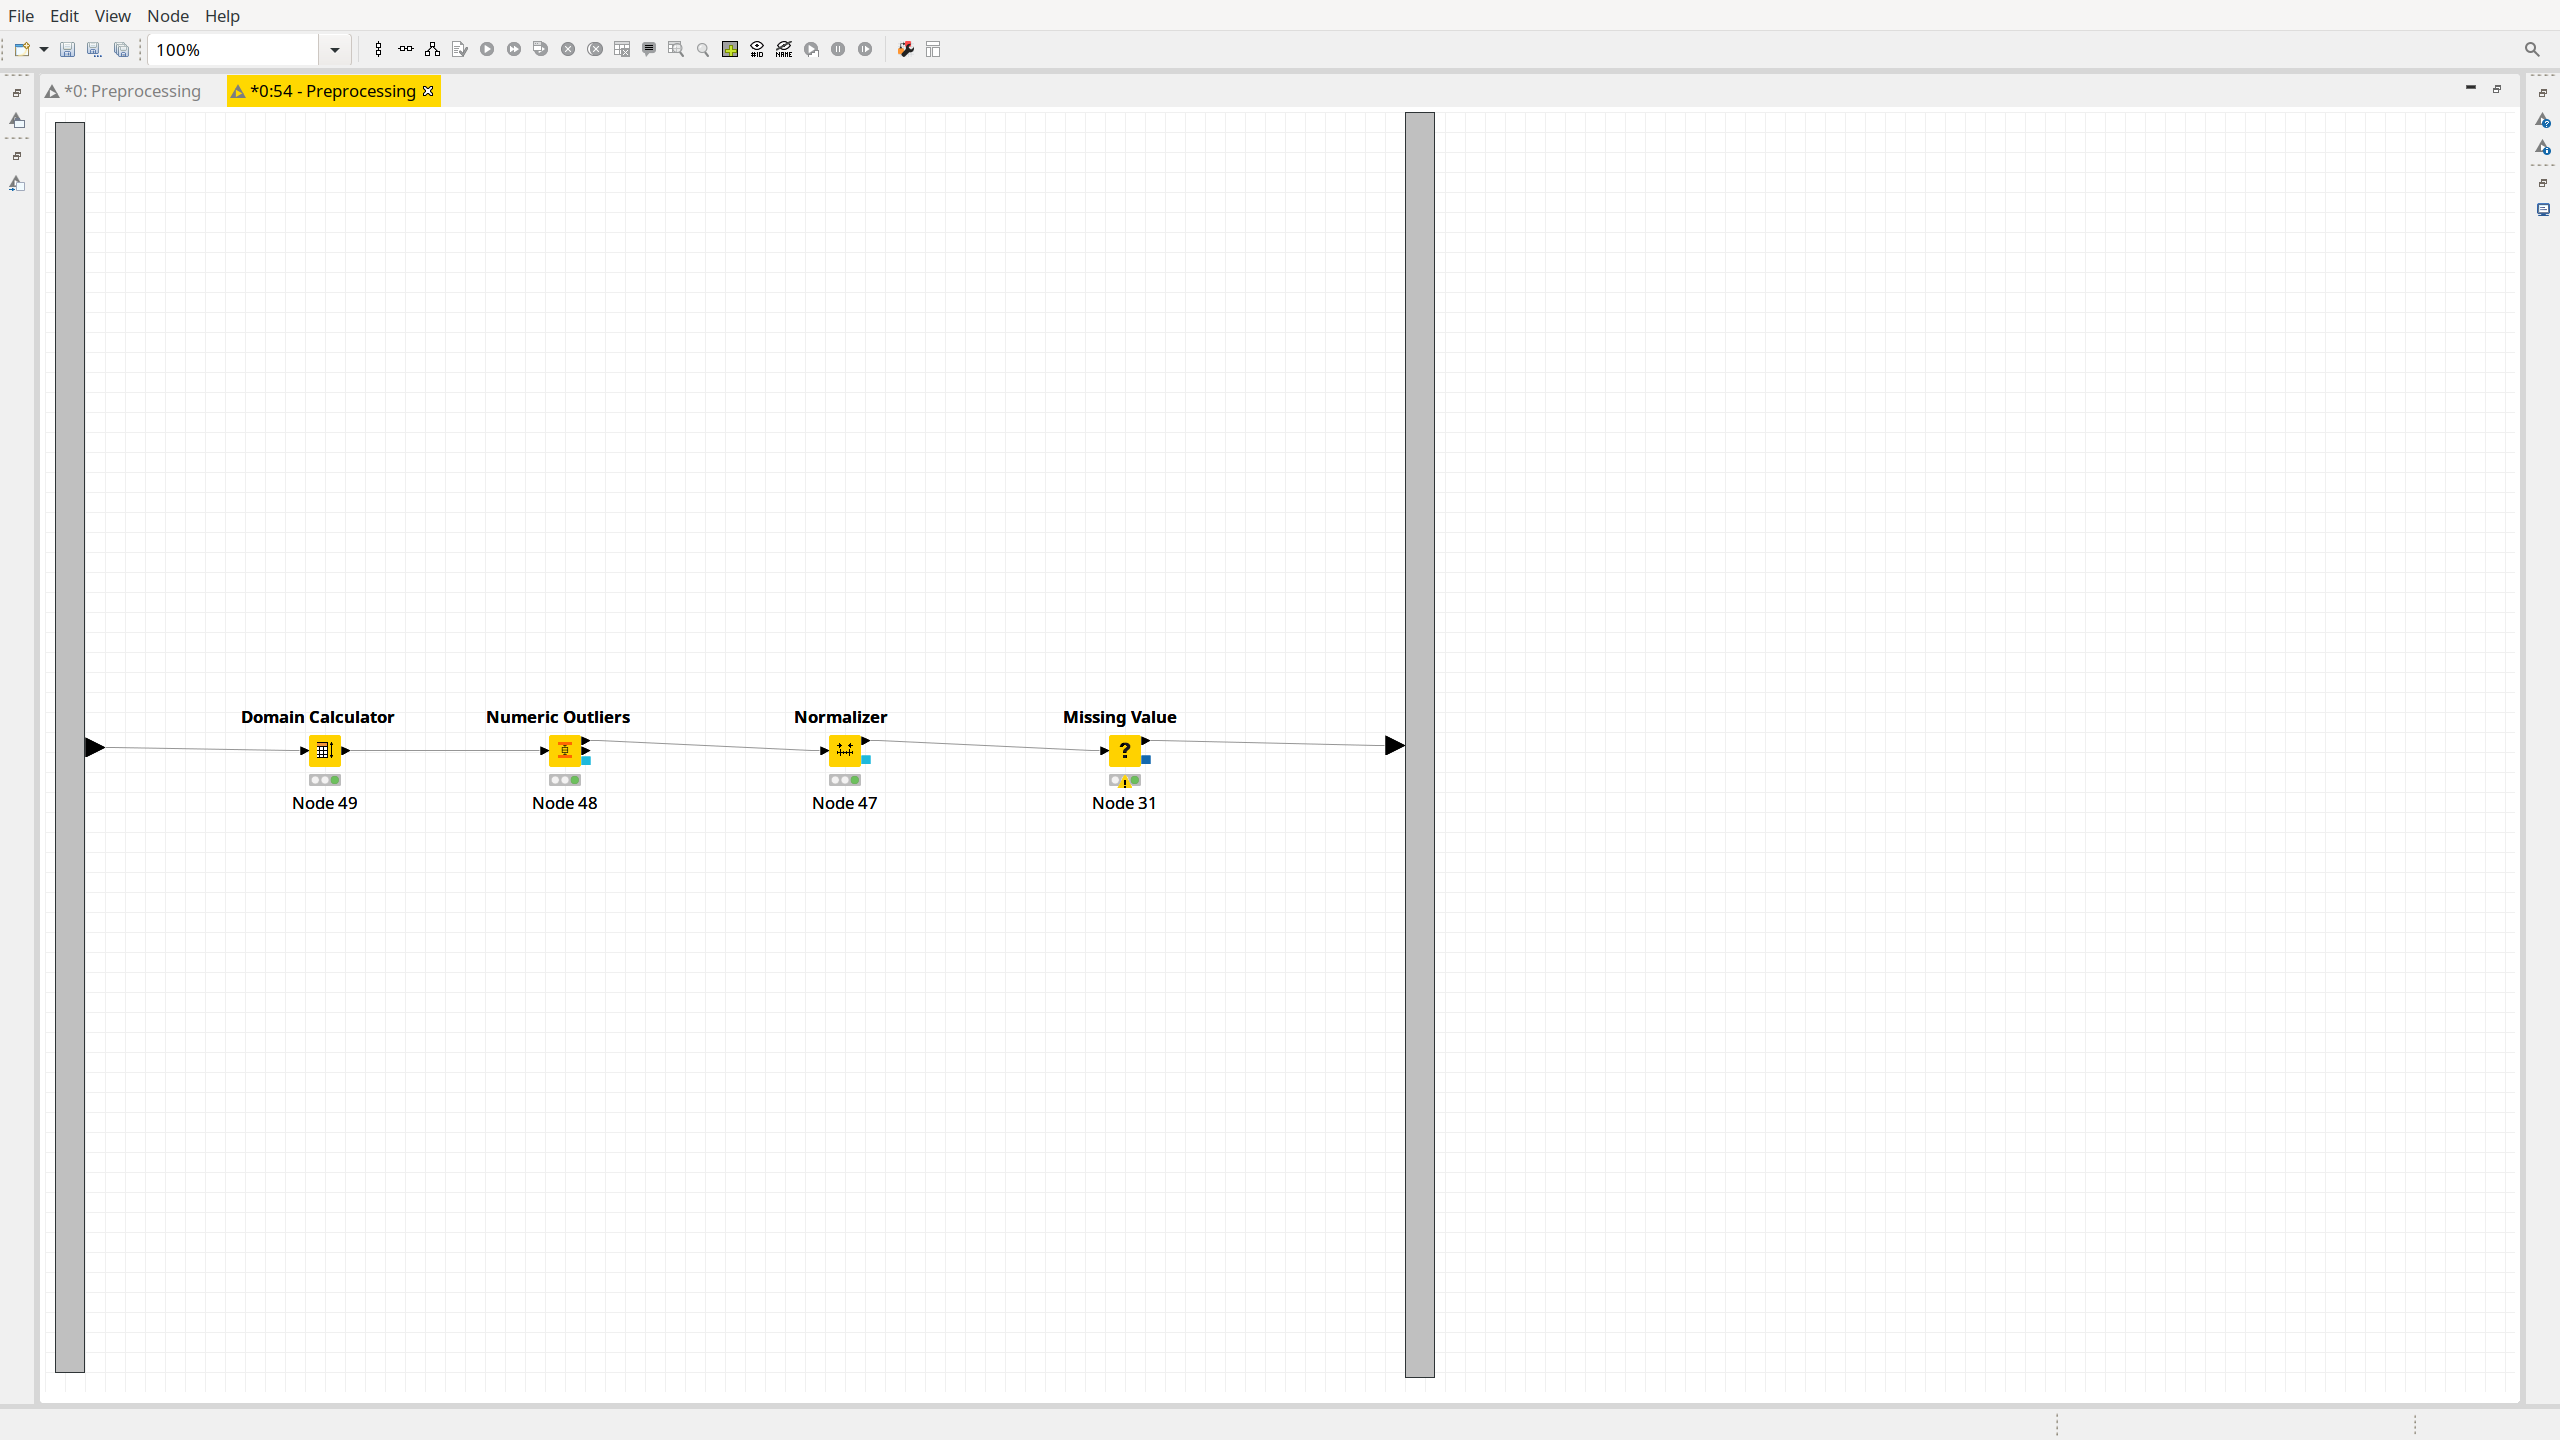
\includegraphics[width=1.0\textwidth]{\ipPreprocessing/preprocessing.png}
	\caption{Flujo de Preprocesado}
	\label{fig:preprocesing}
\end{figure}


\clearpage
\subsection{Resultados}

\begin{figure}[h!]
	\centering
	\includesvg[width=.8\textwidth]{\ipPreprocessing/preprocessing_roc.svg}
\end{figure}

\vspace{1.5em}

\begin{center}
\resizebox{\textwidth}{!}{  %Usado para ajustar la tabla a los bordes del socumento
\pgfplotstabletypeset[
	col sep={comma},
	string type,
	column type=c,
	columns={Algorithms,TPR,TNR,PPV,Accuracy,F-score,G-mean,AUC},
	every head row/.style={	before row={\rowcolor[gray]{0.9}}, after row=\hline,},
	%every last row/.style={ after row=\bottomrule},
	columns/Algorithms/.style	={column type=l|},
	columns/TPR/.style = {precision = 4,fixed zerofill=true, dec sep align},
	columns/TNR/.style = {precision = 4,fixed zerofill=true, dec sep align},
	columns/PPV/.style = {precision = 4,fixed zerofill=true, dec sep align},
	columns/Accuracy/.style = {precision = 4,fixed zerofill=true, dec sep align},
	columns/F-score/.style = {precision = 4,fixed zerofill=true, dec sep align},
	columns/G-mean/.style = {precision = 4,fixed zerofill=true, dec sep align},
	columns/AUC/.style = {precision = 4,fixed zerofill=true, dec sep align},
]{Cuerpo/\ipPreprocessing/results.csv}
}

\vspace{1.5em}
\resizebox{\textwidth}{!}{  %Usado para ajustar la tabla a los bordes del socumento
\pgfplotstabletypeset[
	col sep={comma},
	string type,
	column type=c,
	columns={Algorithms,Tree Size,Training Size,Max. Values,N. Iters,N. Layers,N. Neurons,N. Trees},
	every head row/.style={	before row={\rowcolor[gray]{0.9}}, after row=\hline,},
	every nth row={1}{before row=\hline},
	columns/Algorithms/.style = {column type=l|},
	columns/Tree Size/.style = {column type=c},
	columns/Training Size/.style = {column type=c},
	columns/Max. Values/.style = {column type=c},
	columns/N. Iters/.style = {column type=c},
	columns/N. Layers/.style = {column type=c},
	columns/N. Neurons/.style = {column type=c},
	columns/N. Trees/.style = {column type=c},
]{Cuerpo/\ipPreprocessing/results.csv}
}
\end{center}


\subsection{Conclusiones}

Con respecto a DT: Se tuvo que marcar la casilla \texttt{Max Nominal Split} dentro de la configuración de DT porque de lo contrario el consumo de memoria de knime se disparaba y el proceso excedia la pila y abortaba(Error de knime: Java Heap Space). Esto explica su notable empeoramiento.

Los resultados de KNN son los que mas mejoran hasta el punto de ser el mejor en todas las métricas excepto en la tasa de acierto de la clase positiva. Como ya se ha comentado KNN es un algoritmo basado en distancias y sufre mucho si las variables no están en la misma escala. Podemos con mucha confianza afirmar la hipótesis formulada en la sección \ref{sec:general-considerations} que achacaba los malos resultados de KNN a una falta de normalización.

Por otra parte los resultados de NB también mejoran considerablemente. Los valores perdidos ya se gestionaban en los resultados base porque el algoritmo no sabe trabajar con ellos y la el algoritmo es bastante robusto frente a outliers . El causante de la mejora es la normalización. El algoritmo que utiliza \href{https://hub.knime.com/knime/extensions/org.knime.features.base/latest/org.knime.base.node.mine.bayes.naivebayes.learner3.NaiveBayesLearnerNodeFactory4}{knime} en su implementación es \texttt{Gaussian Bayesian Model}. Este modelo, como su nombre indica, utiliza la distribución gaussiana o normal para estimar el valor de las variable numéricas. La normalización que se aplico es \texttt{z-score} por lo tanto las variables sigue una distribución gaussiana y esto ayuda enormemente al algoritmo.

Los resultados de ANN se mantiene más o menos igual, en algún caso empeoran un poco(como en el caso de TNR). Nuevamente los valores perdidos ya se gestionaban en los resultados base porque el algoritmo no sabe trabajar con ellos, también se normalizaba en los resultados base y se supone que un porcentaje relativamente pequeño de outliers no debería afectar a los resultados \footcite{annOutliers}. Mirando en el workflow de knime se puede observar que tan sólo se detectaron 9 outliers, es decir, un ínfima parte de la base de datos. Por lo tanto no soy capar de explicar este desmejora de los resultados si no es por azar.

Por último está el caso de RF que mejora sustancialmente en TPR a costa del desplome de FPR. Las nuevas variables incluídas con el nodo \texttt{Domain Calculator} parecen polarizar la hipótesis final. En cualquier caso e irónicamente puede considerarse que la hipótesis obtenida es la mejor ciñéndose al criterio establecido en \ref{sec:tanzania-results} lo cual no parece lo más sensato en este caso tan extremo.



\section{Interpretación de Resultados}

\subsection{Heart Failure Prediction}

\begin{figure}[h!]
	\centering
	\includegraphics[width=.37\textwidth]{\ipHeartFailure/dt\_view.png}
	\caption{Atributos Utilizados en el Primer Split de DT en el dataset \textit{Heart Failure Prediction}}%
\end{figure}

\begin{figure}[h!]
\centering
\pgfplotstabletypeset[
	col sep={comma},
	string type,
	column type=l,
	text special chars={\_},
	columns={atributes,splits (level 0),splits (level 1),splits (level 2)},
	every head row/.style={	before row={\rowcolor[gray]{0.9}}, after row=\hline },
	every nth row={1}{before row=\hline},
	% columns/atribute/.style = {column type=l|},
	% columns/#splits (level 0)/.style = {column type=c},
	% columns/#splits (level 1)/.style = {column type=c},
	% columns/#splits (level 2)/.style = {column type=c},
]{Cuerpo/\ipHeartFailure/rf_view.csv}
\caption[]{Atributos y su Numero de Splits por Nivel en Random Forest en el dataset \textit{Heart Failure Prediction} \footnotemark}%
\end{figure}
\footnotetext{No se ha conseguido que el paquete que se está utilizando para portar las tablas de CSV a latex trate correctamente el símbolo \_. Es por este motivo que aparecen en las tablas como un punto flotante.}

En el primero de los datasets la variable utilizada por DT en el primer split es \texttt{ST\_Slope} que representa la pendiete del segmento ST en durante el pico del ejercicio. En el segundo nivel las variables utilizadas son \texttt{ChestPainType} y \texttt{MaxHR} que representan respectivamente el tipo de dolor de pecho y el ritmo cardiaco máximo respectivamente. Por último, en el tercer nivel que más muestras acumula la variable seleccionada para el desarrollo del árbol es \texttt{Sex}.

Por otra parte los atributos más utilizados por los árboles generados por RF en la primera división son, en orden, \texttt{ChestPainType}, \texttt{ST\_Slope}, \texttt{ExerciseAngina} y \texttt{Choresterol}. \texttt{ExerciseAngina} representa el dolor de angina en el pecho causado por la reducción del flujo de sangre al corazón durante el ejercicio. Los más utilizados en el segundo nivel son \texttt{ST\_Slope}, \texttt{ChestPainType}, \texttt{Choresterol}, \texttt{MaxHR} y \texttt{Sex}.

Reuniendo la información aportada por ambos clasificadores podemos afirmar que los atributos que mas afectan en el diagnóstico de una enfermedad cardiovascular son \texttt{ST\_Slope} y \texttt{ChestPainType}. El segundo atributo no es una sorpresa, es bien conocido que el dolor de pecho de estilo característico puede estar ligado a un infarto pero el primero si que es una sorpresa.


\subsection{Mobile Price Classification}

\begin{figure}[h!]
	\centering
	\includegraphics[width=.36\textwidth]{\ipMobilePrice/dt\_view.png}
	\caption{Atributos Utilizados en el Primer Split de DT en el dataset \textit{Mobile Price Classification}}%
\end{figure}

\begin{figure}[h!]
\centering
\pgfplotstabletypeset[
	col sep={comma},
	string type,
	column type=l,
	text special chars={\_},
	columns={atributes,splits (level 0),splits (level 1),splits (level 2)},
	every head row/.style={	before row={\rowcolor[gray]{0.9}}, after row=\hline },
	every nth row={1}{before row=\hline},
	% columns/atribute/.style = {column type=l|},
	% columns/#splits (level 0)/.style = {column type=c},
	% columns/#splits (level 1)/.style = {column type=c},
	% columns/#splits (level 2)/.style = {column type=c},
]{Cuerpo/\ipMobilePrice/rf_view.csv}
\caption{Atributos y su Numero de Splits por Nivel en Random Forest en el dataset \textit{Mobile Price Classification}}%
\end{figure}

En el segundo dataset la variable utilizada en el primer y segundo split es \texttt{ram} que representa el tama en Megabytes de la memoria de acceso aleatorio del teléfono. En el tercer nivel los atributos utilizados son \texttt{px\_height} y \texttt{battery\_power} que representan el tamaño de la pantalla a lo alto en pixeles y el tamaño de la batería en mAh.

Los  atributos más utilizados por los árboles generados por RF en la primera y segunda división son, en orden, \texttt{ram}, \texttt{battery\_power}, \texttt{px\_height} y \texttt{fc}. \texttt{fc} representa los megapixeles de la camara principal.

Las componentes \href{https://www.lanacion.com.ar/tecnologia/cuales-son-los-5-componentes-mas-caros-de-un-celular-nid2088336/}{más caros} en un teléfono móvil son la pantalla, la RAM y la cámara luego tiene sentido que sean los atributos principales utilizados por los clasificadores para predecir el precio. Además, aunque la batería no sea uno de los componentes más caros si que es uno de los más demandados y por lo tanto también marca la diferencia en el precio de los teléfonos.


\subsection{Bank Marketing}

\begin{figure}[h!]
	\centering
	\includegraphics[width=.42\textwidth]{\ipBankMarketing/dt\_view.png}
	\caption{Atributos Utilizados en el Primer Split de DT en el dataset \textit{Bank Marketing}}%
\end{figure}

\begin{figure}[h!]
\centering
\pgfplotstabletypeset[
	col sep={comma},
	string type,
	column type=l,
	columns={atributes,splits (level 0),splits (level 1),splits (level 2)},
	every head row/.style={	before row={\rowcolor[gray]{0.9}}, after row=\hline },
	every nth row={1}{before row=\hline},
	% columns/atribute/.style = {column type=l|},
	% columns/#splits (level 0)/.style = {column type=c},
	% columns/#splits (level 1)/.style = {column type=c},
	% columns/#splits (level 2)/.style = {column type=c},
]{Cuerpo/\ipBankMarketing/rf_view.csv}
\caption{Atributos y su Numero de Splits por Nivel en Random Forest en el dataset \textit{Bank Marketing}}%
\end{figure}

En \textit{Bank Marketing} el atributo usado en la separación del primer nivel es \texttt{nr.employed} en el segundo nivel es \texttt{duration} que representa la duración de la última llamada establecida con el cliente y en el tercer nivel que acumula mayor concentración es \texttt{month} que representa el último mes que se tuvo contacto con el cliente.

En RF los atributos más relevantes tanto en el primer nivel como en el segundo son \texttt{pdays}, \texttt{poutcome}, \texttt{nr.employed} y \texttt{euribor3m} donde \texttt{pdays} representa el número de días transcurridos tras el último contancto con el cliente en una campaña publicitaria pasada y \texttt{poutcome} es representa el exito de la última campaña publicitaria.

Parece que el atributo más relevante es, sin duda \texttt{nr.employed} que representaba el número de empleados.


\subsection{Tanzania Watter Pump}

\begin{figure}[h!]
	\centering
	\includegraphics[width=.48\textwidth]{\ipTanzania/dt\_view.png}
	\caption{Atributos Utilizados en el Primer Split de DT en el dataset \textit{Tanzania Watter Pump}}%
\end{figure}

\begin{figure}[h!]
\centering
\pgfplotstabletypeset[
	col sep={comma},
	string type,
	column type=l,
	text special chars={\_},
	columns={atributes,splits (level 0),splits (level 1),splits (level 2)},
	every head row/.style={	before row={\rowcolor[gray]{0.9}}, after row=\hline },
	every nth row={1}{before row=\hline},
	% columns/atribute/.style = {column type=l|},
	% columns/#splits (level 0)/.style = {column type=c},
	% columns/#splits (level 1)/.style = {column type=c},
	% columns/#splits (level 2)/.style = {column type=c},
]{Cuerpo/\ipTanzania/rf_view.csv}
\caption{Atributos y su Numero de Splits por Nivel en Random Forest en el dataset \textit{Tanzania Watter Pump}}%
\end{figure}

En el último dataset el atributo más utilizado en el split del primer nivel de DT es \texttt{quantity\_group} que representa la cantidad de agua de la bomba. En el segundo nivel el atributo utilizado es \texttt{waterpoint\_type} que representa el tipo de poza.

En RF los atributos más importantes en la definición del primer nivel de los árboles son \texttt{quantity}, \texttt{waterpoint\_type}, \texttt{quantity\_group} y \texttt{waterpoint\_type\_group}. Por último los más relevantes en el segundo nivel son \texttt{extraction\_type}, \texttt{quantity}, \texttt{waterpoint\_type}, \texttt{quantity\_group}.

Los atributos más relevantes en este dataset son los relacionados con la cantidad de agua del pozo, es decir, \texttt{quantity} y \texttt{quantity\_group} y los el tipo de poza, es decir \texttt{waterpoint\_type}. Lo cual tiene sentido puesto que cuanta más agua más tiene que trabajar la bomba y más probabilidades hay de que se estropee e igualmente el tipo de poza condiciona el uso de la bomba y puede provocar un desgaste mayor o menor según cual sea.

\end{document}